\documentclass[12pt,a4paper]{book}%

%_____Options utilisees____________
\usepackage{indentfirst}
%\usepackage{a4}
%\usepackage{amstex}
%\usepackage{amssymb}
\input{epsf}
\usepackage{makeidx}
\usepackage{newlfont}%times} % 
%\usepackage{fancyheadings}

\usepackage{graphicx,html}

%___________________________________

\newcommand{\Rset}{{\cal R}}
\newcommand{\Nset}{{\cal N}}
\newcommand{\Zset}{{\cal Z}}

\makeindex

%______Entete de chaque page________
%\pagestyle{fancyplain}
\newlength{\dimfig}\setlength{\dimfig}{0.55\textwidth}
%\addtolength{\headwidth}{0.3cm}

\renewcommand{\chaptermark}[1]{\markboth{#1}{#1}}
\renewcommand{\sectionmark}[1]{\markright{\thesection\ #1}}

%\lhead[\fancyplain{ }{ }]{\fancyplain{ }{\bf\rightmark}}
%\rhead[\fancyplain{ }{\bf\leftmark}]{\fancyplain{ }{ }}
%\lfoot[\bf \thepage]{Time-Frequency Toolbox User's Guide}
%\rfoot[]{\bf \thepage}
%\cfoot[]{}
%\setlength{\headrulewidth}{0pt}

%___________________________________
%%%%%%%%%%%%%%%%%%%%%%% headline routines %%%%%%%%%%%%%%%%%%%%%%%%%%%% 
%
%  \pagestyle{STYLE}     : sets the page style of the current and succeeding
%                          pages to STYLE
%
%  \thispagestyle{STYLE} : sets the page style of the current page only
%                          to STYLE
%
%  To define a page style STYLE, you must define \ps@STYLE to set the page 
%  style parameters.  
%  
%  HOW A PAGE STYLE MAKES RUNNING HEADS AND FEET:
%  
% The \ps@... command defines the macros \@oddhead, \@oddfoot,
% \@evenhead, and \@evenfoot to define the running heads and feet.  
% (See output routine.)  To make headings determined by the sectioning
% commands, the page style defines the commands \chaptermark,
% \sectionmark, etc., where \chaptermark{TEXT} is called by \chapter to
% set a mark.  The \...mark commands and the \...head macros are defined
% with the help of the following macros.  (All the \...mark commands
% should be initialized to no-ops.)

\newlength{\pagewidth}
\setlength{\pagewidth}{\textwidth}
%\addtolength\pagewidth\marginparwidth
%\addtolength\pagewidth\marginparsep

\makeatletter

\def\ps@myheadings{
\def\@oddfoot{$\overline{\hfill\hbox{\it Time-Frequency Toolbox 
Tutorial, \today}}$}
\def\@oddhead{}
%\makebox[\textwidth][l]{\underline{\hbox to \pagewidth{\bf
%\firstmark\hfill\thepage}}}}%
\def\@evenfoot{$\overline{\hbox{
\thepage\quad F. Auger, P. Flandrin, P. Gon\c{c}alv\`es, 
O. Lemoine\hfill}}$} %
\def\@evenhead{}
%\makebox[\textwidth][r]
%{\underline{\hbox to \pagewidth{\bf\hfill\@lhead}}}}%
\def\chaptermark##1{
%\let\protect\noexpand
\mark{}\def\@lhead{##1}}%
\def\sectionmark##1{{\let\protect\noexpand\mark{\thesection 
    \hskip 1em##1}}}}

%%%%%%%%%%%%%%%%%%%%%%%%%%%%%%%%%%%%%%%%%%%%%%%%%%%%%%%%%%%%%%%%%%%%% 

\begin{htmlonly}
\title{Time-frequency toolbox -- Tutorial}
\author{Fran\c{c}ois Auger, Patrick Flandrin, Paulo Gon\c{c}alv\`es and Olivier Lemoine\\[5mm] CNRS (France), Rice University (USA)}
\date{1995--1996}
\end{htmlonly}

\begin{document}

\begin{htmlonly}
\maketitle
\end{htmlonly}

\begin{latexonly}
\pagestyle{empty}
% This is part of the TFTB Tutorial.
% Copyright (C) 1996 CNRS (France) and Rice University (US).
% See the file tutorial.tex for copying conditions.

\thispagestyle{empty}

\begin{figure}[htb]
\centerline{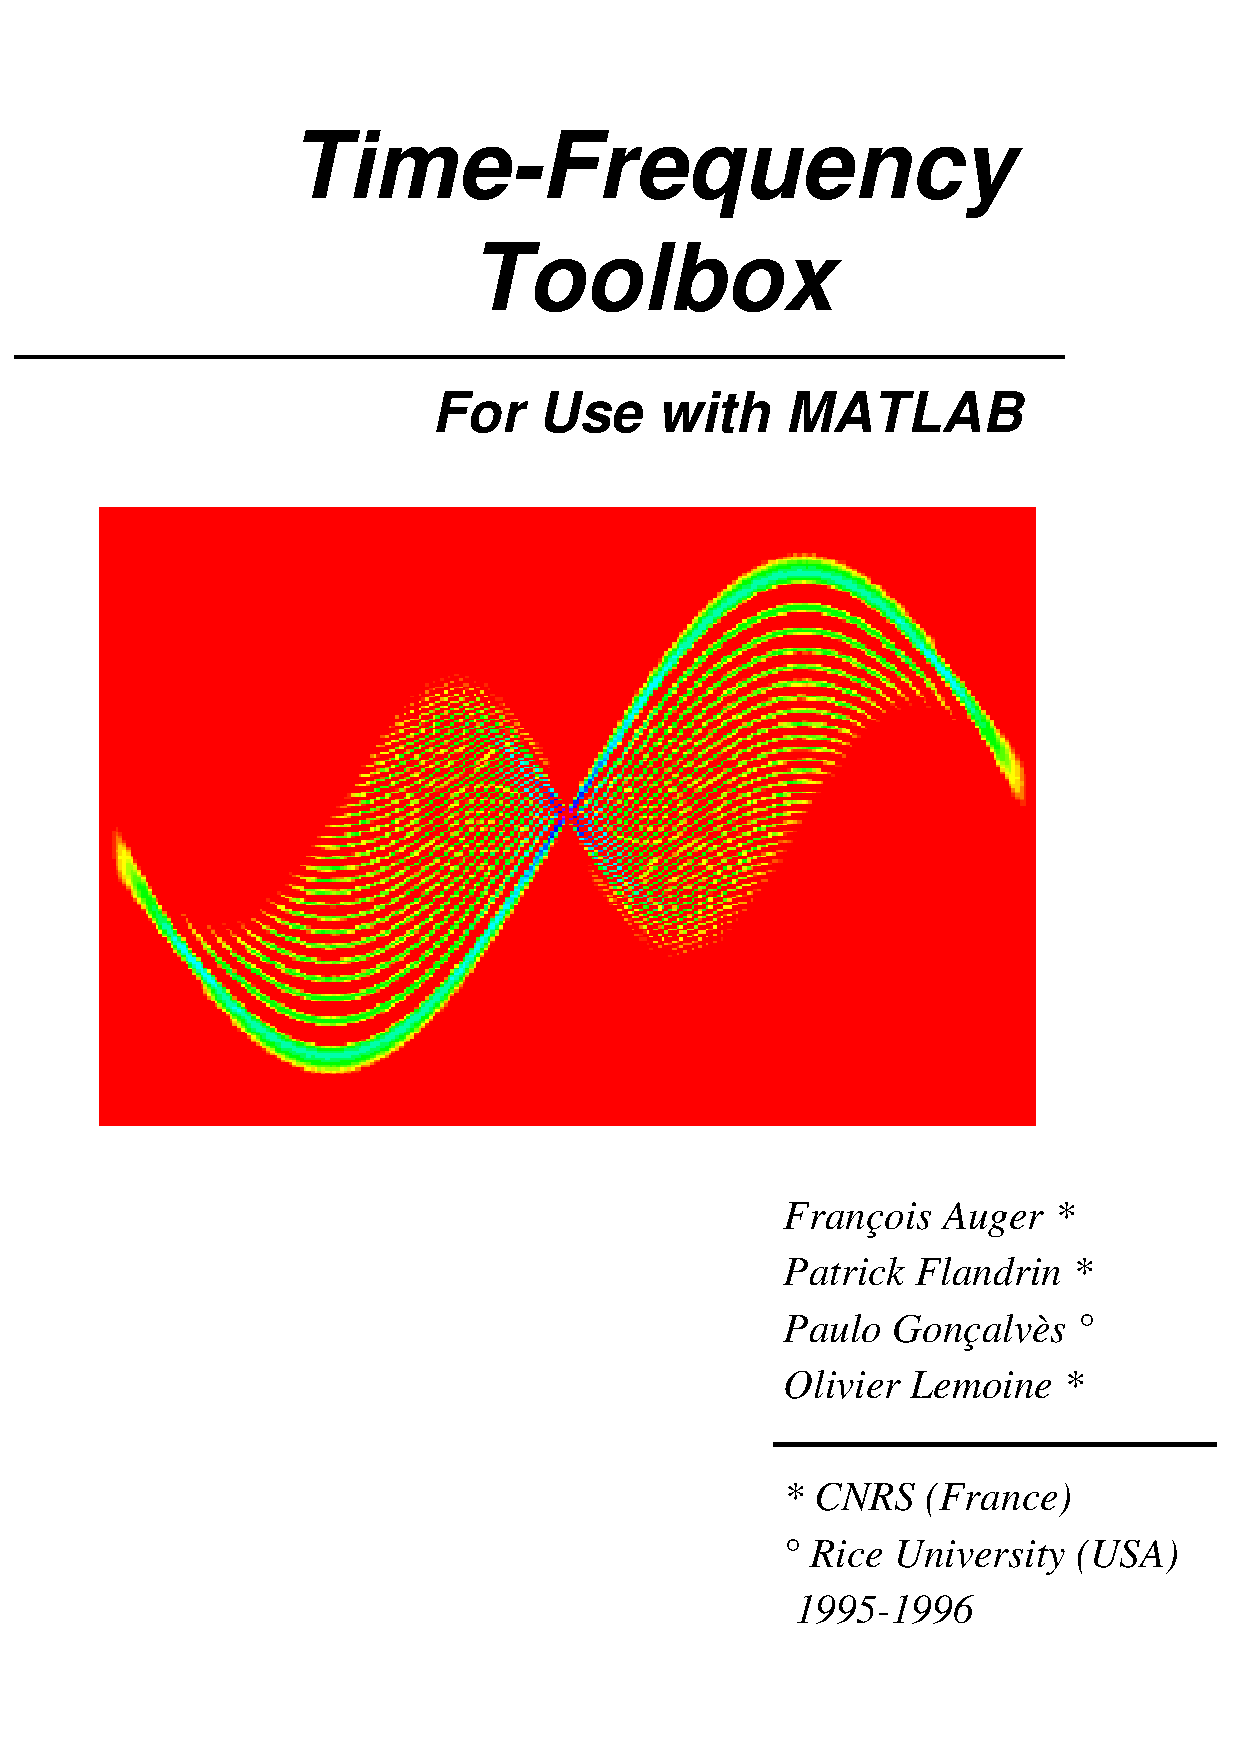
\includegraphics[width=16.8cm,height=23.8cm]{figure/covertu}}
\end{figure}



\end{latexonly}

\cleardoublepage

\begin{htmlonly}
\chapter*{Forewords}
\end{htmlonly}

\centerline{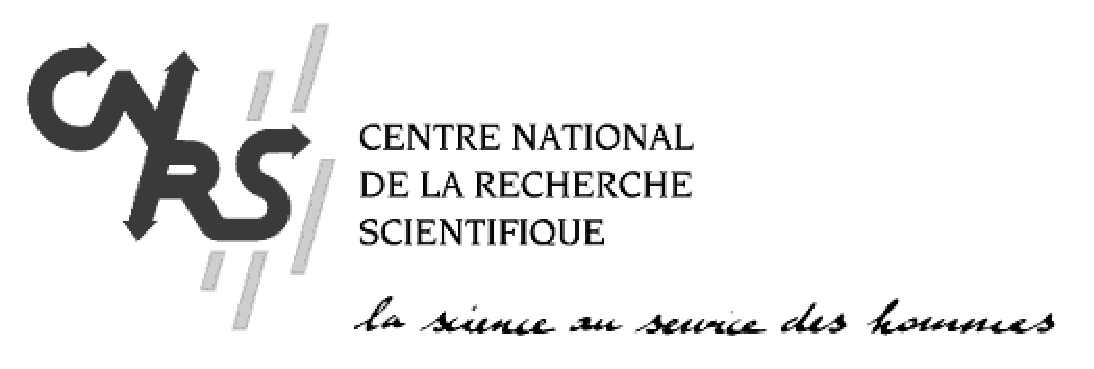
\includegraphics[width=5cm]{figure/cnrs}\hspace{2cm}
            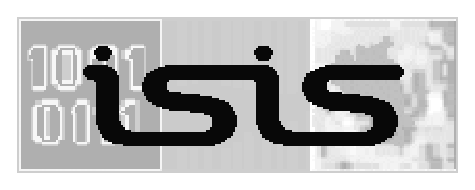
\includegraphics[width=5cm]{figure/isis}}

\vspace{2 cm}
Copyright (C)  1996 CNRS (France) and Rice University (USA).\\
Permission is granted to copy, distribute and/or modify this document
under the terms of the GNU Free Documentation License, Version 1.2
or any later version published by the Free Software Foundation;
with no Invariant Sections, no Front-Cover Texts, and no Back-Cover
Texts.  A copy of the license is included in the section entitled "GNU
Free Documentation License".

\vspace{2 cm}
The Time-Frequency Toolbox has been mainly developed under the auspices of
the French CNRS ({\em Centre National de la Recherche Scientifique}). It
results from a research effort conducted within its Groupements de
Recherche "Traitement du Signal et Images" (O. Macchi) and "Information,
Signal et Images" (J.-M. Chassery). Parts of the Toolbox have also been
developed at Rice University, when one of the authors (PG) was visiting the
Department of Electrical and Computer Engineering, supported by NSF.
Supporting institutions are gratefully acknowledged, as well as M.
Guglielmi, M. Najim, R. Settineri, R.G. Baraniuk, M. Chausse, D. Roche,
E. Chassande-Mottin, O. Michel and P. Abry for their help at different 
phases of the development.

\cleardoublepage

\tableofcontents
\cleardoublepage
\pagestyle{myheadings}
\chapter{Introduction}
% This is part of the TFTB Tutorial.
% Copyright (C) 1996 CNRS (France) and Rice University (US).
% See the file tutorial.tex for copying conditions.

\section{Presentation}
%~~~~~~~~~~~~~~~~~~~~~:eps:

  The Time-Frequency Toolbox is a collection of M-files developed for the
analysis of non-stationary signals using time-frequency distributions.
This toolbox includes two groups of files :

\begin{itemize}
\item the signal generation files, which allow the synthesis of
numerous kinds of non-stationary signals ;
\item the processing files, including the time-frequency distributions
and other related processing functions.
\end{itemize}
	
  As usual under MATLAB, each function of the toolbox has a help entry that
you can refer to by typing
\begin{verbatim}
      >> help name_of_the_file
\end{verbatim}
at the prompt of the matlab command window. In almost every case, a simple
example is given, which facilitates the use of the function.

  Seven demonstration M-files are also available, which provide sequences
of examples illustrating the possibilities of the Time-Frequency Toolbox,
and following closely the plan of this tutorial. These files are :

\begin{center}
\begin{tabular}{|c|c|}
\hline tfdemo  & Main menu of the demonstration\\
\hline \hline tfdemo1 & Introduction\\
\hline tfdemo2 & Non-stationary signals\\
\hline tfdemo3 & Linear time-frequency representations\\
\hline tfdemo4 & Cohen's class time-frequency distributions\\
\hline tfdemo5 & Affine class time-frequency distributions\\
\hline tfdemo6 & Reassigned time-frequency distributions\\
\hline tfdemo7 & Extraction of information\\
\hline
\end{tabular}
\end{center}

  The aim of this Tutorial is to present the way to use the Time-Frequency
Toolbox, and also to introduce the reader in an illustrative and friendly
way to the theory of time-frequency analysis. We advise the reader, when
looking at a chapter of this tutorial, to run simultaneously the
corresponding demonstration file. In this way, he will have a good
understanding of the Toolbox.


\section{Background, system requirements and\\ installation}
%~~~~~~~~~~~~~~~~~~~~~~~~~~~~~~~~~~~~~~~~~~~~~~~~~~~~~~~~~
  This Toolbox is primarily intended for researchers and engineers with
some knowledge on signal processing theory. In particular, the concepts of
Fourier transform, Shannon sampling and stationarity are important to
understand the following features.

  The Time-Frequency Toolbox assumes that MATLAB v.4.2c (or a later version)
is present on your system, as well as the Signal Processing Toolbox v.3.0
(or a later version).

  Instructions for installing this toolbox on a workstation or a large
machine are found in the MATLAB Installation Guide. Instructions for
installing on micro computers are found in the MATLAB User's Guide.


\section{Introductory examples}
%~~~~~~~~~~~~~~~~~~~~~~~~~~~~~~
\subsection{Example 1}
%'''''''''''''''''''''

 Let us consider first a signal with constant amplitude, and with a linear
frequency modulation varying from 0 to 0.5 in normalized frequency (ratio
of the frequency in Hertz to the sampling frequency, with respect to the
Shannon sampling theorem). This signal is called a chirp, and as its
frequency content is varying with time, it is a non-stationary signal. To
obtain such a signal, we can use the M-file \index{\ttfamily
fmlin}{\ttfamily fmlin.m}, which generates a linear frequency modulation
(see fig. \ref{In2fig1})\,:
\begin{verbatim}
     >> sig1=fmlin(128,0,0.5);
     >> plot(real(sig1));
\end{verbatim}
\begin{figure}[htb]
\epsfxsize=10cm
\epsfysize=6cm
\centerline{\epsfbox{figure/in2fig1.eps}}
\caption{\label{In2fig1}Linear frequency modulation (chirp)}
\end{figure}
From this time-domain representation, it is difficult (except for
experienced specialists) to say what kind of modulation is contained in
this signal : what are the initial and final frequencies, is it a linear,
parabolic, hyperbolic\ldots frequency modulation ?

If we now consider the energy spectrum of this signal {\ttfamily sig1} by
squaring the modulus of its Fourier transform (using the {\ttfamily fft}
function) (see fig. \ref{In2fig2}),
\begin{verbatim}
     >> dsp1=fftshift(abs(fft(sig1)).^2); 
     >> plot((-64:63)/128,dsp1);        
\end{verbatim}
\begin{figure}[htb]
\epsfxsize=10cm
\epsfysize=6cm
\centerline{\epsfbox{figure/in2fig2.eps}}
\caption{\label{In2fig2}Energy spectrum of the chirp}
\end{figure}
we still can not say, from this plot, anything about the evolution in time
of the frequency content. This is due to the fact that the Fourier
transform is a decomposition on complex exponentials, which are of infinite
duration and completely unlocalized in time. Time information is in fact
encoded in the phase of the Fourier transform (which is simply ignored by
the energy spectrum), but their interpretation is not straightforward and
their direct extraction is faced with a number of difficulties such as
phase unwrapping.  In order to have a more informative description of such
signals, it would be better to directly represent their frequency content
while still keeping the time description parameter : this is precisely the
aim of time-frequency analysis. To illustrate this, let us try the
Wigner-Ville distribution on this signal (see fig. \ref{In2fig3})\,:
\begin{verbatim}
     >> tfrwv(sig1);
\end{verbatim}
\begin{figure}[htb]
\epsfxsize=10cm
\epsfysize=8cm
\centerline{\epsfbox{figure/in2fig3.eps}}
\caption{\label{In2fig3}Wigner-Ville distribution of the chirp}
\end{figure}
Without going into details about this representation (it will be developed
in the following), we can see that the linear progression of the frequency
with time, from 0 to 0.5, is clearly shown.

  If we now add some complex white gaussian noise on this signal, using the
M-files \index{\ttfamily noisecg}{\ttfamily noisecg.m} and \index{\ttfamily
sigmerge}{\ttfamily sigmerge.m}, with a 0\,dB signal to noise ratio (see
fig. \ref{In2fig4}),
\begin{verbatim}
     >> sig2=sigmerge(sig1,noisecg(128),0);
     >> plot(real(sig2));
\end{verbatim}
\begin{figure}[htb]
\epsfxsize=10cm
\epsfysize=6cm
\centerline{\epsfbox{figure/in2fig4.eps}}
\caption{\label{In2fig4}Chirp embedded in a 0 dB white gaussian noise}
\end{figure}
and consider the spectrum of it (see fig. \ref{In2fig5})\,:
\begin{verbatim}
     >> dsp2=fftshift(abs(fft(sig2)).^2); 
     >> plot((-64:63)/128,dsp2);        
\end{verbatim}
\begin{figure}[htb]
\epsfxsize=10cm
\epsfysize=6cm
\centerline{\epsfbox{figure/in2fig5.eps}}
\caption{\label{In2fig5}Energy spectrum of the noisy chirp}
\end{figure}
it is worse than before to interpret these plots. On the other hand, the
Wigner-Ville distribution still show quite clearly the linear progression
of the frequency with time (see fig. \ref{In2fig6})\,: 
\begin{verbatim}
     >> tfrwv(sig2);
\end{verbatim}
\begin{figure}[htb]
\epsfxsize=10cm
\epsfysize=8cm
\centerline{\epsfbox{figure/in2fig6.eps}}
\caption{\label{In2fig6}Wigner-Ville distribution of the noisy chirp}
\end{figure}


\subsection{Example 2} 
%'''''''''''''''''''''

The second example we consider is a bat sonar signal, recorded with a
sampling frequency of 230.4\,kHz and an effective bandwidth of [8\,kHz,
80\,kHz] (this recording was part of the research program RCP 445
supported by CNRS (Centre National de la Recherche Scientifique, France)
\cite{FLA86}).

  First, load the signal from the MAT-file {\ttfamily bat.mat} (see
fig. \ref{In2fig7})\,: 
\begin{verbatim}
     >> load bat
     >> t0=linspace(0,2500/2304,2500);   
     >> plot(t0,bat); xlabel('Time [ms]');
\end{verbatim}
\begin{figure}[htb]
\epsfxsize=10cm
\epsfysize=6cm
\centerline{\epsfbox{figure/in2fig7.eps}}
\caption{\label{In2fig7}Sonar signal from a bat}
\end{figure}
From this plot, we can not say precisely what is the frequency content at
each time instant $t$ ; similarly, if we look at its spectrum (see
fig. \ref{In2fig8}), 
\begin{verbatim}
     >> dsp=fftshift(abs(fft(bat)).^2);
     >> f0=(-1250:1249)*230.4/2500;
     >> plot(f0,dsp); xlabel('Frequency [kHz]');
\end{verbatim}
\begin{figure}[htb]
\epsfxsize=10cm
\epsfysize=6cm
\centerline{\epsfbox{figure/in2fig8.eps}}
\caption{\label{In2fig8}Energy spectrum of the bat sonar signal}
\end{figure}
we can not say at what time the signal is located around 38\,kHz, and at
what time around 40\,kHz (you can use the zoom function to see more
precisely what is happening around these frequencies ; see the Matlab
Reference Guide). Let us now consider a representation called the pseudo
Wigner-Ville distribution, applied on the most interesting part of this
signal (this distribution was obtained with the M-file \index{\ttfamily
tfrpwv}{\ttfamily tfrpwv.m}, stored in the matrix {\ttfamily tfr} and saved
with the signal in the MAT-file {\ttfamily bat.mat} ; the corresponding
time- and frequency- samples {\ttfamily t} and {\ttfamily f} where also
saved on {\ttfamily bat.mat}) (see fig. \ref{In2fig9})\,:
\begin{verbatim}
     >> contour(t,f,tfr,5); axis('xy'); 
     >> xlabel('Time [ms]'); ylabel('Frequency [kHz]'); 
     >> title('TFRPWV of a bat signal');  
\end{verbatim}
\begin{figure}[htb]
\epsfxsize=10cm
\epsfysize=8cm
\centerline{\epsfbox{figure/in2fig9.eps}}
\caption{\label{In2fig9}Pseudo-WVD of the bat sonar signal}
\end{figure}
We then have a nice description of its spectral content varying with time :
it is a narrow-band signal, whose frequency content is decreasing from
around 55\,kHz to 38\,kHz, with a non-linear frequency modulation
(approximately of hyperbolic shape).

\subsection{Example 3} 
%'''''''''''''''''''''

The last introductory example presented here is a transient signal embedded
in a -5\,dB white gaussian noise. This transient signal is a constant
frequency modulated by a one-sided exponential amplitude (see
fig. \ref{In2fig10})\,: 
\begin{verbatim}
     >> trans=amexpo1s(64).*fmconst(64);
     >> sig=[zeros(100,1) ; trans ; zeros(92,1)];
     >> sign=sigmerge(sig,noisecg(256),-5);
     >> plot(real(sign));
     >> dsp=fftshift(abs(fft(sign)).^2);
     >> plot((-128:127)/256,dsp);
\end{verbatim}
\begin{figure}[htb]
\epsfxsize=10cm
\epsfysize=8cm
\centerline{\epsfbox{figure/in2fig10.eps}}
\caption{\label{In2fig10}Time- and frequency- representation of a noisy
transient signal}
\end{figure}
From these representations, it is difficult to localize precisely the
signal in the time-domain as well as in the frequency domain.  Now let us
have a look at the spectrogram of this signal calculated using the M-file
\index{\ttfamily tfrsp}{\ttfamily tfrsp.m} (see fig. \ref{In2fig11})\,:
\begin{verbatim}
     >> tfrsp(sign);
\end{verbatim}
\begin{figure}[htb]
\epsfxsize=10cm
\epsfysize=8cm
\centerline{\epsfbox{figure/in2fig11.eps}}
\caption{\label{In2fig11}Spectrogram of the noisy transient signal}
\end{figure}
the transient signal appears distinctly around the normalized frequency
0.25, and between time points 125 and 160.



\chapter{Non stationary signals}
% This is part of the TFTB Tutorial.
% Copyright (C) 1996 CNRS (France) and Rice University (US).
% See the file tutorial.tex for copying conditions.

  This chapter presents some useful definitions that constitute the
background of time-frequency analysis (most of the information presented in
this tutorial are extracted from \cite{FLA93}). After a brief recall on
time-domain and frequency-domain representations, we introduce the concepts
of time and frequency localizations, time-bandwidth product and the
constraint associated to this product (the Heisenberg-Gabor
inequality). Then, the instantaneous frequency and the group delay are
presented as a first solution to the problem of time localization of the
spectrum. We carry on by defining non-stationarity from its opposite,
stationarity, and show how to synthesize such non-stationary signals with
the toolbox. Finally, we show that in the case of multi-component signals,
these mono-dimensional functions (instantaneous frequency and group delay)
are not sufficient to represent these signals ; a two-dimensional
description (function of time {\em and} frequency) is necessary.


\section{Time representation and frequency representation}
%~~~~~~~~~~~~~~~~~~~~~~~~~~~~~~~~~~~~~~~~~~~~~~~~~~~~~~~~~
  The time representation is usually the first (and the most natural)
description of a signal we consider, since almost all physical signals are
obtained by receivers recording variations with time.

  The frequency representation, obtained by the {\it Fourier transform}
\index{Fourier transform}
\[X(\nu) = \int_{-\infty}^{+\infty} x(t)\ e^{-j2\pi \nu t}\ dt,\]
is also a very powerful way to describe a signal, mainly because the
relevance of the concept of frequency is shared by many domains (physics,
astronomy, economics, biology \ldots) in which periodic events occur.

  But if we look more carefully at the spectrum $X(\nu)$, it can be viewed
as the coefficient function obtained by expanding the signal $x(t)$ into
the family of infinite waves, $\exp\{j2\pi \nu t\}$, which are completely
unlocalized in time. Thus, the spectrum essentially tells us which
frequencies are contained in the signal, as well as their corresponding
amplitudes and phases, but does not tell us at which times these
frequencies occur.


\section{Localization and the Heisenberg-Gabor\\ principle}
%~~~~~~~~~~~~~~~~~~~~~~~~~~~~~~~~~~~~~~~~~~~~~~~~~~~~~
\markright{Localization and the Heisenberg-Gabor principle}
  A simple way to characterize a signal simultaneously in time and in
frequency is to consider its mean localizations and dispersions in each of
these representations. This can be obtained by considering $|x(t)|^2$ and
$|X(\nu)|^2$ as probability distributions, and looking at their mean values
and standard deviations : \index{average time}\index{average
frequency}\index{time spreading}\index{frequency spreading}
%\begin{xalignat}{2}
$$
\begin{array}{rcll}
t_m   &=& \frac{1}{E_x}\ \int_{-\infty}^{+\infty} t\ |x(t)|^2\ dt  & 
\mbox{\it average time}\\	  
\nu_m &=& \frac{1}{E_x}\ \int_{-\infty}^{+\infty} \nu\ |X(\nu)|^2\ d\nu  & 
\mbox{\it average frequency}\\ 
T^2   &=& \frac{
4\pi}{E_x}\ \int_{-\infty}^{+\infty} (t-t_m)^2\ |x(t)|^2\ dt
&  \mbox{\it time spreading}\\ 
B^2   &=& \frac{4\pi}{E_x}\ \int_{-\infty}^{+\infty} (\nu-\nu_m)^2\
|X(\nu)|^2\ d\nu &  \mbox{\it frequency spreading}
\end{array}
$$
%\end{eqnarray*}
%\end{xalignat}

where $E_x$ is the \index{energy} {\it energy} of the signal, assumed to be
finite (bounded) :
\[E_x = \int_{-\infty}^{+\infty} |x(t)|^2\ dt < + \infty.\]
Then a signal can be characterized in the time-frequency plane by its mean
position $(t_m, \nu_m)$ and a domain of main energy localization whose area
is proportional to the {\it time-bandwidth product} $T\times B$.\\
\index{time-bandwidth product}

\subsection{Example 1} 
%'''''''''''''''''''''
\label{ex1}
These time and frequency localizations can be evaluated thanks to the
M-files \index{\ttfamily loctime}{\ttfamily loctime.m} and \index{\ttfamily
locfreq}{\ttfamily locfreq.m} of the Toolbox. The first one gives the
average time center ($t_m$) and the duration ($T$) of a signal, and the
second one the average normalized frequency ($\nu_m$) and the normalized
bandwidth ($B$). For example, for a linear chirp with a gaussian amplitude
modulation, we obtain (see fig. \ref{Ns2fig1})\,:
\begin{verbatim}
     >> sig=fmlin(256).*amgauss(256);
     >> [tm,T]=loctime(sig)           --->  tm=128     T=32
     >> [num,B]=locfreq(sig)          --->  num=0.249  B=0.0701
\end{verbatim}
\begin{figure}[htb]
\epsfxsize=10cm
\epsfysize=8cm
\centerline{\epsfbox{figure/ns2fig1.eps}}
\caption{\label{Ns2fig1}Linear chirp with a gaussian amplitude modulation}
\end{figure}

  One interesting property of this product $T\times B$ is that it is lower
bounded :
\[T \times B \geq 1.\]
\index{Heisenberg-Gabor inequality} This constraint, known as the {\it
Heisenberg-Gabor inequality}, illustrates the fact that a signal can not
have simultaneously an arbitrarily small support in time and in
frequency. This property is a consequence of the definition of the Fourier
transform. The lower bound $T\times B = 1$ is reached for gaussian
functions :
\[x(t) = C \exp{[-\alpha(t - t_m)^2 + j2\pi \nu_m(t-t_m)]}\]
%with $C \in \mathbb{R}$, $\alpha \in \mathbb{R}_{+}$. Therefore, the
with $C \in \Rset$, $\alpha \in \Rset_{+}$. Therefore, the
gaussian signals are those which minimize the time-bandwidth product
according to the Heisenberg-Gabor inequality.\\

\subsection{Example 2}
%'''''''''''''''''''''

 To check the Heisenberg-Gabor inequality numerically, we consider a
gaussian signal and calculate its time-bandwidth product (see
fig. \ref{Ns2fig2})\,: 
\begin{verbatim}
     >> sig=amgauss(256);
     >> [tm,T]=loctime(sig); 
     >> [fm,B]=locfreq(sig);
     >> [T,B,T*B]             --->  T=32  B=0.0312  T*B=1	       
\end{verbatim}
\begin{figure}[htb]
\epsfxsize=10cm
\epsfysize=8cm
\centerline{\epsfbox{figure/ns2fig2.eps}}
\caption{\label{Ns2fig2}gaussian signal : lower bound of the
Heisenberg-Gabor inequality}
\end{figure}
Hence, the time-bandwidth product obtained, when using the file
\index{\ttfamily amgauss}{\ttfamily amgauss.m}, is minimum.

\section{Instantaneous frequency}
%~~~~~~~~~~~~~~~~~~~~~~~~~~~~~~~~
\label{anasig}
\index{instantaneous frequency}
\index{analytic signal}
\index{Hilbert transform}
  Another way to describe a signal simultaneously in time and in frequency
is to consider its {\it instantaneous frequency}. In order to introduce such a
function, we must define first the concept of {\it analytic signal}.

  For any real valued signal $x(t)$, we associate a complex valued signal
$x_a(t)$ defined as
\[x_a(t) = x(t) + j HT(x(t))\]
where $HT(x)$ is the {\it Hilbert transform} of $x$ ($x_a$ can be obtained
using the M-file {\ttfamily hilbert.m} of the Signal Processing
Toolbox). $x_a(t)$ is called the analytic signal associated to $x(t)$. This
definition has a simple interpretation in the frequency domain since $X_a$
is a single-sided Fourier transform where the negative frequency values
have been removed, the strictly positive ones have been doubled, and the DC
component is kept unchanged :
\begin{eqnarray*}
	X_a(\nu) = 0 \ \ \ \ \ \ &\mbox{if}& \nu < 0 \\
	X_a(\nu) = X(0)\ \ &\mbox{if}& \nu = 0 \\
	X_a(\nu) = 2X(\nu) &\mbox{if}& \nu > 0 
\end{eqnarray*}
($X$ is the Fourier transform of $x$, and $X_a$ the Fourier transform of
$x_a$). Thus, the analytic signal can be obtained from the real signal by
forcing to zero its spectrum for the negative frequencies, which do not
alter the information content since for a real signal, $X(-\nu)=X^*(\nu)$.

\index{instantaneous amplitude}
 From this signal, it is then possible to define in a unique way the
concepts of {\it instantaneous amplitude} and {\it instantaneous frequency} by :
\begin{eqnarray*}
a(t) &=& |x_a(t)| \ \ \ \ \ \ \ \ \ \ \ \mbox{\it  instantaneous amplitude} \\
f(t) &=& \frac{1}{2\pi} \frac{d\arg{x_a(t)}}{dt}\ \mbox{\it  instantaneous
frequency}  
\end{eqnarray*}
An estimation of the instantaneous frequency is given by the M-file
\index{\ttfamily instfreq}{\ttfamily instfreq.m} of the Time-Frequency
toolbox :\\

   {\bf Example} (see fig. \ref{Ns3fig1})

\begin{verbatim}
     >> sig=fmlin(256); t=(3:256);
     >> ifr=instfreq(sig); plotifl(t,ifr);
\end{verbatim}
\begin{figure}[htb]
\epsfxsize=10cm
\epsfysize=6cm
\centerline{\epsfbox{figure/ns3fig1.eps}}
\caption{\label{Ns3fig1}Estimation of the instantaneous frequency of a
linear chirp}
\end{figure}
As we can see from this plot, the instantaneous frequency shows with
success the evolution with time of the frequency content of this signal.


\section{Group delay}
%~~~~~~~~~~~~~~~~~~~~
\index{group delay}
  The instantaneous frequency characterizes a local frequency behavior as a
function of time. In a dual way, the local time behavior as a function of
frequency is described by the {\it group delay} :
\[t_x(\nu) = -\frac{1}{2\pi}  \frac{d\arg{X_a(\nu)}}{d \nu}.\]
This quantity measures the average time arrival of the frequency $\nu$. The
M-file \index{\ttfamily sgrpdlay}{\ttfamily sgrpdlay.m} of the
Time-Frequency Toolbox gives an estimation of the group delay of a signal
(do not mistake it for the file {\ttfamily grpdelay.m} of the signal
processing toolbox which gives the group delay of a digital filter). For
example, with signal {\ttfamily sig} of the previous example, we obtain
(see fig. \ref{Ns4fig1})\,:
\begin{verbatim}
     >> sig=fmlin(256); fnorm=0:.05:.5;
     >> gd=sgrpdlay(sig,fnorm); plot(gd,fnorm);
\end{verbatim}

\begin{figure}[htb]
\epsfxsize=10cm
\epsfysize=6cm
\centerline{\epsfbox{figure/ns4fig1.eps}}
\caption{\label{Ns4fig1}Estimation of the group delay of the previous chirp}
\end{figure}

Be careful of the fact that in general, instantaneous frequency and group
delay define two different curves in the time-frequency plane. They are
approximatively identical only when the time-bandwidth product $T\times B$
is large. To illustrate this point, let us consider a simple example. We
calculate the instantaneous frequency and group delay of two signals, the
first one having a large $T\times B$ product, and the second one a small
$T\times B$ product (see fig. \ref{Ns4fig2})\,:
\begin{verbatim}
     >> t=2:255; 
     >> sig1=amgauss(256,128,90).*fmlin(256,0,0.5);
     >> [tm,T1]=loctime(sig1); [fm,B1]=locfreq(sig1); 
     >> T1*B1              --->  T1*B1=15.9138
     >> ifr1=instfreq(sig1,t); f1=linspace(0,0.5-1/256,256);
     >> gd1=sgrpdlay(sig1,f1); plot(t,ifr1,'*',gd1,f1,'-')
     >> sig2=amgauss(256,128,30).*fmlin(256,0.2,0.4);
     >> [tm,T2]=loctime(sig2); [fm,B2]=locfreq(sig2); 
     >> T2*B2              --->  T2*B2=1.224
     >> ifr2=instfreq(sig2,t); f2=linspace(0.2,0.4,256);
     >> gd2=sgrpdlay(sig2,f2); plot(t,ifr2,'*',gd2,f2,'-')
\end{verbatim}
\begin{figure}[htb]
\epsfxsize=10cm
\epsfysize=8cm
\centerline{\epsfbox{figure/ns4fig2.eps}}
\caption{\label{Ns4fig2}Estimation of the instantaneous frequency (stars)
and group delay (line) of two different chirps with different amplitude
modulations. The first plot corresponds to a large $T\times B$ product
while the second corresponds to a small one}
\end{figure}
On the first plot, the two curves are almost superimposed (i.e. the
instantaneous frequency is the inverse transform of the group delay),
whereas on the second plot, the two curves are clearly different.


\section{About stationarity}
%~~~~~~~~~~~~~~~~~~~~~~~~~~~
\index{stationarity}
  Before talking about non-stationarity, which is a 'non-property', we must
define what we call {\it stationarity}.

  A deterministic signal is said to be {\it stationary} if it can be
written as a discrete sum of sinusoids :

\begin{eqnarray*}
x(t)&=&\sum_{k \in \Nset} A_k \cos{[2\pi \nu_k t + \Phi_k]} \ \ \ \
\mbox{ for a real signal} \\   
x(t)&=&\sum_{k \in \Nset} A_k \exp{[j(2\pi \nu_k t + \Phi_k)]} 
\mbox{for a complex signal}  
\end{eqnarray*}
i.e. as a sum of elements which have constant instantaneous amplitude and
instantaneous frequency.

  In the random case, a signal $x(t)$ is said to be {\it wide-sense
stationary} (or stationary up to the second order) if its expectation is
independent of time and its autocorrelation function $E[x(t_1)x^*(t_2)]$
depends only on the time difference $t_2-t_1$. We can then show that the
associated analytic signal has constant instantaneous amplitude and
frequency expectations, which can be connected to the deterministic case.

\index{non-stationarity} 
So a signal is said to be {\it non-stationary} if one of these fundamental
assumptions is no longer valid. For example, a finite duration signal, and
in particular a {\it transient signal} (for which the length is short
compared to the observation duration), is non-stationary.


\section{How to synthesize a mono-component non-stationary signal}
%~~~~~~~~~~~~~~~~~~~~~~~~~~~~~~~~~~~~~~~~~~~~~~~~~~~~~~~~~~~~~~~~~
  One part of the Time-Frequency Toolbox is dedicated to the generation of
non-stationary signals. In that part, three groups of M-files are available\,:

\begin{enumerate}
\item The first one allows to synthesize different amplitude
modulations. These M-files begin with the prefix '{\ttfamily am}'. For
example, {\ttfamily amrect.m} computes a rectangular amplitude modulation,
{\ttfamily amgauss.m} a gaussian amplitude modulation \ldots

\item The second one proposes different frequency modulations.  These
M-files begin with '{\ttfamily fm}'. For example, {\ttfamily fmconst.m} is
a constant frequency modulation, {\ttfamily fmhyp.m} a hyperbolic frequency
modulation \ldots

\item The third one is a set of pre-defined signals. Some of them begin
with '{\ttfamily ana}' because these signals are analytic (for example
{\ttfamily anastep, anabpsk, anasing} \ldots), other have special names
({\ttfamily doppler, atoms} \ldots).
\end{enumerate}

  The first two groups of files can be combined to produce a large class of
non-stationary signals, multiplying an amplitude modulation and a frequency
modulation.\\

 {\bf Examples}  

We can multiply the linear frequency modulation of Example 1 (see page
\pageref{ex1}) by a gaussian amplitude modulation (see
fig. \ref{Ns6fig1})\,:
\begin{verbatim}
     >> fm1=fmlin(256,0,0.5);
     >> am1=amgauss(256);
     >> sig1=am1.*fm1; plot(real(sig1));
\end{verbatim}
\begin{figure}[htb]
\epsfxsize=10cm
\epsfysize=6cm
\centerline{\epsfbox{figure/ns6fig1.eps}}
\caption{\label{Ns6fig1}Mono-component non-stationary signal with a linear
frequency modulation and a gaussian amplitude modulation}
\end{figure}
By default, the signal is centered on the middle (256/2=128), and its
spread is $T=32$. If you want to center it at an other position {\ttfamily
t0}, just replace {\ttfamily am1} by {\ttfamily amgauss(256,t0)}. A second
example can be to multiply a pure frequency (constant frequency modulation)
by a one-sided exponential window starting at {\ttfamily t=100} (see
fig. \ref{Ns6fig2})\,:
\begin{verbatim}
     >> fm2=fmconst(256,0.2);
     >> am2=amexpo1s(256,100);
     >> sig2=am2.*fm2; plot(real(sig2));
\end{verbatim}
\begin{figure}[htb]
\epsfxsize=10cm
\epsfysize=6cm
\centerline{\epsfbox{figure/ns6fig2.eps}}
\caption{\label{Ns6fig2}Mono-component non-stationary signal with a
constant frequency modulation and a one-sided exponential amplitude
modulation} 
\end{figure}

As a third example of mono-component non-stationary signal, we can consider
the M-file \index{\ttfamily doppler}{\ttfamily doppler.m} : this function
generates a modelization of the signal received by a fixed observer from a
moving target emitting a pure frequency (see fig. \ref{Ns6fig3}).
\begin{verbatim}
     >> [fm3,am3]=doppler(256,200,4000/60,10,50);
     >> sig3=am3.*fm3; plot(real(sig3));
\end{verbatim}
\begin{figure}[htb]
\epsfxsize=10cm
\epsfysize=6cm
\centerline{\epsfbox{figure/ns6fig3.eps}}
\caption{\label{Ns6fig3}Doppler signal}
\end{figure}
This example corresponds to a target (a car for instance) moving straightly
at the speed of 50\,m/s, and passing at 10\,m from the observer (the
radar\,!). The rotating frequency of the engine is 4000\,revolutions per
minute, and the sampling frequency of the radar is 200\,Hz.\\

  In order to have a more realistic modelization of physical signals, we
may need to add some complex noise on these signals. To do so, two M-files
\index{\ttfamily noisecg}({\ttfamily noisecg} an \index{\ttfamily
noisecu}{\ttfamily noisecu}) of the Time-Frequency Toolbox are proposed :
{\ttfamily noisecg.m} generates a complex white or colored gaussian noise,
and {\ttfamily noisecu.m}, a complex white uniform noise. For example, if
we add complex colored gaussian noise on the signal {\ttfamily sig1} with a
signal to noise ratio of -10\,dB (see fig. \ref{Ns6fig4})
\begin{verbatim}
     >> noise=noisecg(256,.8);
     >> sign=sigmerge(sig1,noise,-10); plot(real(sign));
\end{verbatim}
\begin{figure}[htb]
\epsfxsize=10cm
\epsfysize=6cm
\centerline{\epsfbox{figure/ns6fig4.eps}}
\caption{\label{Ns6fig4}Gaussian transient signal ({\ttfamily sig1})
embedded in a -10\,dB colored gaussian noise} 
\end{figure}
the deterministic signal {\ttfamily sig1} is now almost imperceptible from
the noise.


\section{What about multi-component non-stationary signals ?}
%~~~~~~~~~~~~~~~~~~~~~~~~~~~~~~~~~~~~~~~~~~~~~~~~~~~~~~~~~~~~  
  The notion of instantaneous frequency implicitly assumes that, at each
time instant, there exists only a single frequency component. A dual
restriction applies to the group delay : the implicit assumption is that a
given frequency is concentrated around a single time instant. Thus, if
these assumptions are no longer valid, which is the case for most of the
multi-component signals, the result obtained using the instantaneous
frequency or the group delay is meaningless.\\

  {\bf Example} 

For example, let us consider the superposition of two linear frequency
modulations :
\begin{verbatim}
     >> N=128; x1=fmlin(N,0,0.2); x2=fmlin(N,0.3,0.5);
     >> x=x1+x2;
\end{verbatim}
At each time instant $t$, an ideal time-frequency representation should
represent two different frequencies with the same amplitude. The results
obtained using the instantaneous frequency and the group delay are of
course completely different, and therefore irrelevant (see
fig. \ref{Ns7fig1})\,: 
\begin{verbatim}
     >> ifr=instfreq(x); subplot(211); plot(ifr);
     >> fn=0:0.01:0.5; gd=sgrpdlay(x,fn); 
     >> subplot(212); plot(gd,fn);
\end{verbatim}
\begin{figure}[htb]
\epsfxsize=10cm
\epsfysize=6cm
\centerline{\epsfbox{figure/ns7fig1.eps}}
\caption{\label{Ns7fig1}Estimation of the instantaneous frequency (first
plot) and group-delay (second plot) of a multi-component signal}
\end{figure}
So these one-dimensional representations, instantaneous frequency and group
delay, are not sufficient to represent all the non-stationary signals. A
further step has to be made towards two-dimensional mixed representations,
jointly in time and in frequency. Even if no gain of information can be
expected since it is all contained in the time or in the frequency
representation, we can obtain a better structuring of this information, and
an improvement in the intelligibility of the representation.

  To have an idea of what can be made with a time-frequency decomposition,
let us anticipate the following and have a look at the result obtained on
this signal with the Short Time Fourier Transform (see
fig. \ref{Ns7fig2})\,:
\begin{verbatim}
     >> tfrstft(x);
\end{verbatim}
\begin{figure}[htb]
\epsfxsize=10cm
\epsfysize=8cm
\centerline{\epsfbox{figure/ns7fig2.eps}}
\caption{\label{Ns7fig2}Squared modulus of the short-time Fourier transform
of the previous multi-component non-stationary signal}
\end{figure}
Here two ``time-frequency components'' can be clearly seen, located around
the locus of the two frequency modulations.



\chapter{First class of solutions : the atomic decompositions}
% This is part of the TFTB Tutorial.
% Copyright (C) 1996 CNRS (France) and Rice University (US).
% See the file tutorial.tex for copying conditions.

  As we have seen in the previous chapter, the Fourier transform is not
adapted to the analysis of non-stationary signals since it projects the
signal on infinite waves (sinusoids) which are completely delocalized in
time.  The concepts of instantaneous frequency and group delay are also
inherently unadapted to a large number of non-stationary signals, those
containing more than one elementary component, and in particular noisy
signals. Thus mono-dimensional solutions seem not to be sufficient, and one
has to consider bi-dimensional functions (functions of the variables time
and frequency).

\index{atomic decomposition} \index{short-time Fourier transform} A first
class of such time-frequency representations is given by the {\it atomic
decompositions} (also known as the {\it linear time-frequency
representations}). To introduce this concept, we begin with the {\it
short-time Fourier transform} which has a very intuitive interpretation.


\section{The Short-Time Fourier Transform}
%~~~~~~~~~~~~~~~~~~~~~~~~~~~~~~~~~~~~~~~~~
\subsection{Definition}
%''''''''''''''''''''''
  In order to introduce time-dependency in the Fourier transform, a simple
and intuitive solution consists in pre-windowing the signal $x(u)$ around a
particular time $t$, calculating its Fourier transform, and doing that for
each time instant $t$. The resulting transform, called the {\it short-time
Fourier transform} (STFT, or {\it short-time spectrum}), is
\[F_x(t,\nu;h) = \int_{-\infty}^{+\infty} x(u)\ h^*(u-t)\ e^{-j2\pi \nu u}\
du\] where $h(t)$ is a {\it short time analysis window} (see fig. \ref{At1fig1})
localized around $t=0$ and $\nu=0$.
\begin{figure}[htb]
\epsfxsize=10cm
\epsfysize=6cm
\centerline{\epsfbox{figure/at1fig1.eps}}
\caption{\label{At1fig1}non-stationary signal $x(u)$ and the short-time
window $h^*(u-t)$ centered at time $t$}
\end{figure}
Because multiplication by the relatively short window $h^*(u-t)$
effectively suppresses the signal outside a neighborhood around the
analysis time point $u=t$, the STFT is a "local" spectrum of the signal
$x(u)$ around $t$. Provided that the short-time window is of finite energy,
the STFT is invertible according to
\[x(t) = \frac{1}{E_h}\ \int_{-\infty}^{+\infty} \int_{-\infty}^{+\infty}
F_x(u,\xi;h)\ h(t-u)\ e^{j2\pi t \xi}\ du\ d\xi,\] 
with $E_h=\int_{-\infty}^{+\infty} |h(t)|^2\ dt$.  This relation expresses
that the total signal can be decomposed as a weighted sum of elementary
waveforms
\[h_{t,\nu}(u) = h(u-t)\ \exp{[j2\pi \nu u]}\]
\index{atom} which can be interpreted as ``building blocks" or ``{\it
atoms}". Each atom is obtained from the window $h(t)$ by a translation in
time and a translation in frequency (modulation). The corresponding
transformation group of translations in both time and frequency is called
the {\it Weyl-Heisenberg group}. \label{WHG} \index{Weyl-Heisenberg
group} Fig. \ref{At1fig2} shows two such atoms corresponding to a gaussian
window.
\begin{figure}[htb]
\epsfxsize=10cm
\epsfysize=6cm
\centerline{\epsfbox{figure/at1fig2.eps}}
\caption{\label{At1fig2}Time-frequency atoms\,: two atoms corresponding to
a gaussian window. The STFT is a projection of the analyzed signal on such
atoms which are relatively well localized in time and in frequency}
\end{figure}
The STFT may also be expressed in terms of signal and window spectra\,:
\[F_x(t,\nu;h)=\int_{-\infty}^{+\infty} X(\xi)\ H^*(\xi-\nu)\ \exp{[j\
2\pi(\xi-\nu)t]}\ d\xi\] 
where $X$ and $H$ are respectively the Fourier transforms of $x$ and
$h$. Thus, the STFT $F_x(t,\nu;h)$ can be considered as the result of
passing the signal $x(u)$ through a band-pass filter whose frequency
response is $H^*(\xi-\nu)$, and is therefore deduced from a mother filter
$H(\xi)$ by a translation of $\nu$. So the STFT is similar to a bank of
band-pass filters with constant bandwidth.


\subsection{An example}
%''''''''''''''''''''''
  Let us have a look at the result obtained by applying the STFT on a
speech signal. The signal we consider is a speech signal containing the
word 'GABOR', recorded on 338\,points with a sampling frequency of 1\,kHz
(with respect to the Shannon criterion) (see fig. \ref{At1fig3}).
\begin{verbatim}
     >> load gabor
     >> time=0:337; subplot(211); plot(time,gabor); 
     >> dsp=fftshift(abs(fft(gabor)).^2);
     >> freq=(-169:168)/338*1000; subplot(212); plot(freq,dsp); 
\end{verbatim}
\begin{figure}[htb]
\epsfxsize=10cm
\epsfysize=6cm
\centerline{\epsfbox{figure/at1fig3.eps}}
\caption{\label{At1fig3}Speech signal corresponding to the word
'GABOR'. Time signal (first plot) and its energy spectral density (second
plot)}
\end{figure}
We can not say from this representation what part of the word is
responsible for that peak around 140\,Hz.

Now if we look at the squared modulus of the STFT of this signal, using a
hamming analysis window of 85\,points, we can see some interesting features
(the time-frequency matrix is loaded from the MAT-file because it takes a
long time to be calculated ; we represent only the frequency domain where
the signal is present) (see fig. \ref{At1fig4})\,:
\begin{verbatim}
     >> contour(time,(0:127)/256*1000,tfr); grid;
     >> xlabel('Time [ms]'); ylabel('Frequency [Hz]'); 
     >> title('Squared modulus of the STFT of the word GABOR');
\end{verbatim}
\begin{figure}[htb]
\epsfxsize=10cm
\epsfysize=8cm
\centerline{\epsfbox{figure/at1fig4.eps}}
\caption{\label{At1fig4}Speech signal analyzed in the time-frequency plane}
\end{figure}
The first pattern in the time-frequency plane, located between 30\,ms and
60\,ms, and centered around 150\,Hz, corresponds to the first syllable
'GA'. The second pattern, located between 150\,ms and 250\,ms, corresponds
to the last syllable 'BOR', and we can see that its mean frequency is
decreasing from 140\,Hz to 110\,Hz with time. Harmonics corresponding to
these two fundamental signals are also present at higher frequencies, but
with a lower amplitude.


\subsection{Some properties}
%'''''''''''''''''''''''''''
\begin{itemize}
\item The STFT preserves frequency shifts and time shifts up to a modulation:
\begin{eqnarray*}
y(t) = x(t)\ e^{j2\pi \nu_0 t} &\ \Rightarrow\ & F_y(t,\nu;h)=F_x(t,\nu-\nu_0;h)\\ 
y(t) = x(t-t_0) &\ \Rightarrow\ & F_y(t,\nu;h)=F_x(t-t_0,\nu;h)\ e^{j2\pi t_0 \nu}  
\end{eqnarray*}
     
\item Generalizing what has been said previously, the signal $x(t)$ can be
reconstructed from its STFT with a synthesis window $g(t)$ different from the
analysis window $h(t)$\,:
\[x(t)=\int_{-\infty}^{+\infty} \int_{-\infty}^{+\infty} F_x(u,\xi;h)\
g(t-u)\ e^{j2\pi t \xi}\ du\ d\xi\] 
providing that the windows $g$ and $h$ validate the constraint 
\[\int_{-\infty}^{+\infty} g(t)\ h^*(t)\ dt =1.\]
\end{itemize}

\subsection{Time-frequency resolution}
%''''''''''''''''''''''''''''''''''''''
 The time resolution of the STFT can be obtained by considering for $x$ a
Dirac impulse\,:
\[x(t)=\delta(t-t_0) \ \Rightarrow\  F_x(t,\nu;h)=\exp{[-j2\pi t_0 \nu]}
\ h(t-t_0).\]  
Thus, the time resolution of the STFT is proportional to the effective
duration of the analysis window $h$. Similarly, to obtain the
frequency-resolution, we have to consider a complex sinusoid (a Dirac
impulse in the frequency domain)\,:
\[x(t)=\exp{[j2\pi \nu_0 t]} \ \Rightarrow\  F_x(t,\nu;h)=\exp{[-j2\pi t
\nu_0]}\ H(\nu-\nu_0).\] So the frequency-resolution of the STFT is
proportional to the effective bandwidth of the analysis window
$h$. Consequently, for the STFT, we have a {\it trade-off} between time and
frequency resolutions\,: on one hand, a good time resolution requires a
short window $h(t)$ ; on the other hand, a good frequency resolution
requires a narrow-band filter i.e. a long window $h(t)$. But unfortunately,
these wishes can not be simultaneously granted. This limitation is a
consequence of the Heisenberg-Gabor inequality. Two instructive cases can
be considered\,:
  
\begin{enumerate}
\item The first one corresponds to a perfect time resolution\,: the window
$h(t)$ is chosen as a Dirac impulse\,:
\[h(t)=\delta(t) \ \Rightarrow\  F_x(t,\nu;h)=x(t)\ \exp{[-j2\pi \nu t]}\]   
the STFT is perfectly localized in time, but does not provide any frequency
resolution.\\

  * {\it Example}\,: This can be computed easily using the Time-Frequency
Toolbox\,: we consider for $x$ a linear frequency modulation with a gaussian
amplitude modulation (see fig. \ref{At1fig5}).
\begin{verbatim}
     >> x=real(amgauss(128).*fmlin(128));
     >> h=1;
     >> tfrstft(x,1:128,128,h);
\end{verbatim}
\begin{figure}[htb]
\epsfxsize=10cm
\epsfysize=8cm
\centerline{\epsfbox{figure/at1fig5.eps}}
\caption{\label{At1fig5}Perfect time resolution with the STFT, but with no
frequency resolution : the window $h$ is chosen as a Dirac impulse}
\end{figure}
The signal is perfectly localized in time (a section for a given frequency
of the modulus of the STFT corresponds exactly to the modulus of the
signal), but the frequency resolution is null.

\item The second is that of perfect frequency resolution, obtained with a
constant window
\[h(t)=1\ (H(\nu)=\delta(\nu))\ \ \Rightarrow\ \ F_x(t,\nu;h)=X(\nu)\]
here the STFT reduces to the Fourier transform of $x(t)$, and does not
provide any time resolution (see fig. \ref{At1fig6}).
\begin{verbatim}
     >> h=ones(127,1);
     >> tfrstft(x,1:128,128,h);
\end{verbatim}
\begin{figure}[htb]
\epsfxsize=10cm
\epsfysize=8cm
\centerline{\epsfbox{figure/at1fig6.eps}}
\caption{\label{At1fig6}Perfect frequency resolution with the STFT : the window
$h$ is chosen as a constant}
\end{figure}
The result obtained for $F_x(t,\nu;h)$ is not exactly $X(\nu)$, because the
window $h$ has not an infinite duration. Thus, some side effects appear.
\end{enumerate}

  To illustrate the influence of the shape and length of the analysis
window $h$, we consider two transient signals having the same gaussian
amplitude and constant frequency, with different arrival times (using the
M-file \index{\ttfamily atoms}{\ttfamily atoms.m})\,:
\begin{verbatim}
     >> sig=atoms(128,[45,.25,32,1;85,.25,32,1]);
\end{verbatim}
Here is the result obtained with a Hamming analysis window of 65\,points
(see fig. \ref{At1fig7})\,: 
\begin{verbatim}
     >> h=window(65,'hamming');
     >> tfrstft(sig,1:128,128,h);
\end{verbatim}
\begin{figure}[htb]
\epsfxsize=10cm
\epsfysize=8cm
\centerline{\epsfbox{figure/at1fig7.eps}}
\caption{\label{At1fig7}Two gaussian atoms analyzed by the STFT using a
Hamming window $h$ of 65\,points : it is difficult to discriminate the two
components in time}
\end{figure}
The frequency resolution is very good, but it is almost impossible to
discriminate the two components in time. If we now consider a short Hamming
window of 17\,points (see fig. \ref{At1fig8})
\begin{verbatim}
     >> h=window(17,'hamming');
     >> tfrstft(sig,1:128,128,h);
\end{verbatim}
\begin{figure}[htb]
\epsfxsize=10cm
\epsfysize=8cm
\centerline{\epsfbox{figure/at1fig8.eps}}
\caption{\label{At1fig8}Same gaussian atoms analyzed by the STFT using a
Hamming window $h$ of 17\,points : frequency resolution is poorer, but the
two components can be easily distinguished}
\end{figure}
the frequency resolution is poorer, but the time resolution is sufficiently
good to distinguish the two components. For more information on the choice
of the window, see \cite{HAR78}.


\section{Time-scale analysis and the wavelet transform}
%~~~~~~~~~~~~~~~~~~~~~~~~~~~~~~~~~~~~~~~~~~~~~~~~~~~~~~
  Since the Wavelet Toolbox is fully dedicated to this problem, we will
merely give here some basic definitions which are essential in the next
part to introduce the affine quadratic time-frequency distributions.

\subsection{Definitions and interpretation}
%''''''''''''''''''''''''''''''''''''''''''
\label{CWT}
\index{continuous wavelet transform} \index{wavelets} The idea of the {\it
continuous wavelet transform} (CWT) is to project a signal $x$ on a family
of zero-mean functions (the {\it wavelets}) deduced from an elementary
function (the {\it mother wavelet}) by translations and dilations:
\[T_x(t,a;\Psi)=\int_{-\infty}^{+\infty} x(s)\ \Psi^*_{t,a}(s)\ ds\,:
\mbox{\it Continuous Wavelet Transform}\] where $\Psi_{t,a}(s)=|a|^{-1/2}\
\Psi\left({s-t\over a}\right)$. \index{scale} The variable $a$
corresponds now to a {\it scale} factor, in the sense that taking $|a|>1$
dilates the wavelet $\Psi$ and taking $|a|<1$ compresses $\Psi$. By
definition, the wavelet transform is more a time-scale than a
time-frequency representation. However, for wavelets which are
well localized around a non-zero frequency $\nu_0$ at scale $a = 1$, a
time-frequency interpretation is possible thanks to the formal
identification $\nu={\nu_0\over a}$.
\begin{figure}[htb]
\epsfxsize=10cm
\epsfysize=6cm
\centerline{\epsfbox{figure/at2fig1.eps}}
\caption{\label{At2fig1}Time-scale atoms. The CWT is a projection of the
analyzed signal on such atoms whose time duration is inversely proportional
to the central frequency}
\end{figure}

\label{Qana}
  The basic difference between the wavelet transform and the short-time
Fourier transform is as follows\,: when the scale factor $a$ is changed, the
duration and the bandwidth of the wavelet are both changed but its shape
remains the same. And in contrast to the STFT, which uses a single analysis
window, the CWT uses short windows at high frequencies and long windows at
low frequencies. This partially overcomes the resolution limitation of the
STFT\,: the bandwidth $B$ is proportional to $\nu$, or
\[\frac{B}{\nu}=Q\,: \mbox{ constant}.\]
\index{constant-Q analysis}
We call it a {\it constant-Q analysis}. The CWT can also be seen as a filter
bank analysis composed of band-pass filters with constant relative
bandwidth.


\subsection{Properties}
%''''''''''''''''''''''
\label{affinegroup}
\index{affine group}
\begin{itemize}
\item The wavelet transform is covariant by translation in time and scaling,
which means that
\[ y(t) = \sqrt{|a_0|}\ x(a_0(t-t_0)) \ \Rightarrow\  T_y(t,a;\Psi) =
T_x(a_0^*(t-t_0),a/a_0;\Psi).\] 
The corresponding group of transforms is called the {\it affine group} (to
be compared to the Weyl-Heisenberg group).
  
\item The signal $x$ can be recovered from its continuous wavelet transform
according to the formula
\[x(t) = \int_{-\infty}^{+\infty}\int_{-\infty}^{+\infty} T_x(s,a;\Phi)\
\Psi_{s,a}(t)\ ds\ \frac{da}{a^2}\] 
where $\Phi$ is the {\it synthesis wavelet}, if the following admissibility
condition is verified by $\Phi$ and $\Psi$\,:
\[\int_{-\infty}^{+\infty} \Psi(\nu)\ \Phi^*(\nu)\ \frac{d\nu}{|\nu|}\ =\
1.\] 
 
\item Time and frequency resolutions, like in the STFT case, are related via
the Heisenberg-Gabor inequality. However, in the present case, these two
resolutions depend on the frequency\,: the frequency resolution (resp. time
resolution) becomes poorer (resp. better) as the analysis frequency grows.
\end{itemize}

\section{Sampling considerations}
%~~~~~~~~~~~~~~~~~~~~~~~~~~~~~~~~
\subsection{The discrete STFT}
%'''''''''''''''''''''''''''''
  To reduce the redundancy of the continuous STFT, we can sample it in the
time-frequency plane. Since the atoms used can be deduced from the window
$h(t)$ by translation in time and in frequency, it is natural to sample the
STFT on a rectangular grid\,:
\[F_x[n,m;h]=F_x(nt_0,m\nu_0;h)=\int_{-\infty}^{+\infty} x(u)\
h^*(u-nt_0) \exp{[-j2\pi m \nu_0 u]}\ du \]
$m,n \in \Zset$. The problem is then to choose the values of $t_0$ and $\nu_0$
so as to minimize the redundancy without loosing any information. For that,
we must have
\[t_0\times \nu_0\ \leq\ 1.\]
Then, the atoms ${h_{nt_0,m\nu_0}}$ constitute a discrete over-sampled
family of non orthonormal elements, which is called a {\it frame} : when
$t_0\times \nu_0>1$, the time-frequency plane is not sufficiently "covered" by
the atoms $h_{nt_0,m\nu_0}$, i.e.  there are "gaps" between adjacent
atoms.

  When $t_0\times \nu_0 = 1$, the family of atoms ${h_{nt_0,m\nu_0}}$ can
constitute an {\it orthonormal basis} for an appropriate choice of the
window. But it can be shown that it is impossible to obtain such a basis
with a window $h$ which is well localized in time and in frequency (this
property is known as the {\it Balian-Low obstruction}
\cite{DAU92}). \index{Balian-Low obstruction}Therefore, for a well localized
window $h$ (for example a gaussian window), the reconstruction formula will
not be numerically stable.

  In the discrete case, the reconstruction (synthesis) formula of the
signal from the STFT is then given by
\[x(t) = \sum_n \sum_m F_x[n,m;h]\ g_{n,m}(t)\]
where $g_{n,m}(t)=g(t-nt_0)\ \exp{[j2\pi m \nu_0 t]}$.

This relation is valid provided that the sampling periods $t_0$ and
$\nu_0$, the analysis window $h$ and the synthesis window $g$ are chosen
such that
\[\frac{1}{\nu_0} \sum_n g(t+\frac{k}{\nu_0}-nt_0)\ h^*(t-nt_0)\ =\
\delta_k\ \ \forall t\]
with $\delta_k$ defined as $\delta_0=1$ and $\delta_k=0$ for $k\neq
0$. This condition is far more restrictive than the condition
$\int_{-\infty}^{+\infty} g(t)\ h^*(t)\ dt=1$ required in the continuous case.

  For a sampled signal $x[n]$ whose sampling period is noted $T$, $t_0$ has
to be chosen so that $t_0 = kT$, $k\in \Nset^*$. We then have the
following analysis and synthesis formulae
\begin{eqnarray}
\label{gabcoef}
F_x[n,m;h] &=& \sum_k x[k]\ h^*[k-n]\ \exp{[-j2\pi m k]} \mbox{   for   }
-\frac{1}{2} \leq  m \leq  \frac{1}{2} \\
\label{gabsynth}
      x[k] &=& \sum_n \sum_m F_x[n,m;h]\ g[k-n]\ \exp{[j2\pi m k]}.
\end{eqnarray}
These two relations can be implemented efficiently using a Fast Fourier
Transform (FFT) algorithm.


\subsection{The Gabor Representation}
%''''''''''''''''''''''''''''''''''''
  The reconstruction (synthesis) formula of the STFT is given in the discrete
case by
\[x(t) = \sum_n \sum_m F_x[n,m;h]\ g_{n,m}(t)\]
where $g_{n,m}(t)=g(t-nt_0)\ \exp{[j2\pi m \nu_0 t]}$ defines the {\it
Gabor representation}. \index{Gabor representation}Originally, the
synthesis window $g(t)$ was chosen by Gabor as a gaussian window, because
it maximizes the concentration in the time-frequency plane. But now we
speak of Gabor representation for any normalized window $g$.

\index{Gabor logons} \index{Gabor coefficients} The atoms $g_{n,m}(t)$ are
called the {\it Gabor logons}, and the coefficients $F_x[n,m;h]$, noted
$G_x[n,m]$ in the following, the {\it Gabor coefficients}. Each coefficient
contains an information relative to the time-frequency content of the signal
around the time-frequency location $(n t_0,m \nu_0)$.  The logon $g_{n,m}$
is associated in the time-frequency plane to a rectangular unit area
centered on $(n t_0,m \nu_0)$.

  What about completeness of the Gabor logons $g_{n,m}(t)$ ? As we have
seen before, a necessary but not sufficient condition is that $t_0\
\nu_0\leq 1$. At the critical sampling case $t_0\ \nu_0=1$, the logons are
linearly independent, but are not orthogonal in general (Balian-Low
obstruction). This means that the Gabor coefficients $G_x[n,m]$ are not
simply the projections of $x(t)$ onto the corresponding logons $g_{n,m}(t)$
(i.e. the analysis and synthesis windows $h$ and $g$ can not be the
same). A theoretical solution to this problem is obtained if the windows
$g$ and $h$ are chosen biorthonormal, i.e. if they validate the
{\it biorthonormal condition}
\[ \int_{-\infty}^{+\infty} g_{n,m}(t)\ h^*_{n',m'}(t)\ dt = \delta_{n-n'}\
\ \delta_{m-m'}\] 

\index{biorthonormal window} \index{Zak transform} Then the analysis
formula given before (expression (\ref{gabcoef})) allows the computation of
the Gabor coefficients, and the synthesis formula (expression
(\ref{gabsynth})) the reconstruction of the signal $x(t)$ (to compute the
{\it biorthonormal window} $h$ associated to a given synthesis window $g$,
one can use the {\it Zak transform} \cite{AUS91} : this is the approach
followed in the file \index{\ttfamily tfrgabor}{\ttfamily tfrgabor}, and
the file \index{\ttfamily zak}{\ttfamily zak.m} computes this
transform). From an implementation point of view, this solution is not fully
satisfactory since the computation of the biorthonormal window $h$ is
numerically unstable. So in general, some degree of {\it oversampling} is
considered $(t_0\times \nu_0<1)$, which introduces redundancy in the
coefficients, in order to "smooth" the biorthonormal window $h$, for the
sake of numerical stability. These considerations are closely connected to
the theory of frames.\\

  {\bf Example}

 Let us consider the Gabor coefficients of a linear chirp of N1=256 points
at the critical sampling case, and for a gaussian window of
Ng=33\,points\,:
\begin{verbatim}
     >> N1=256; Ng=33; Q=1; % degree of oversampling.
     >> sig=fmlin(N1); g=window(Ng,'gauss'); g=g/norm(g);
     >> [tfr,dgr,h]=tfrgabor(sig,16,Q,g);
\end{verbatim}
({\ttfamily tfrgabor} generates as first output the squared modulus of the
Gabor representation, as second output the complex Gabor representation,
and as third output the biorthonormal window). When we look at the
biorthonormal window $h$ (see fig. \ref{At3fig1}),
\begin{verbatim}
     >> plot(h); 
\end{verbatim}
\begin{figure}[htb]
\epsfxsize=10cm
\epsfysize=6cm
\centerline{\epsfbox{figure/at3fig1.eps}}
\caption{\label{At3fig1}Biorthonormal window corresponding to the critical
sampling case and to a gaussian synthesis window : numerically unsteady}
\end{figure}
we can see how "bristling" this function is. The corresponding Gabor
decomposition contains all the information about {\ttfamily sig}, but is
not easy to interpret (see fig. \ref{At3fig2})\,:
\begin{verbatim}
     >> t=1:256; f=linspace(0,0.5,128); imagesc(t,f,tfr(1:128,:)); 
     >> xlabel('Time'); ylabel('Normalized frequency'); axis('xy'); 
     >> title('Squared modulus of the Gabor coefficients');
\end{verbatim}
\begin{figure}[htb]
\epsfxsize=10cm
\epsfysize=8cm
\centerline{\epsfbox{figure/at3fig2.eps}}
\caption{\label{At3fig2}Gabor representation of a chirp, at the critical
sampling rate : we have as many coefficients in the time-frequency plane as
in the signal (no redundancy)}
\end{figure}
If we now consider a degree of oversampling of {\ttfamily Q=4} (there are
four times more Gabor coefficients than signal samples), the biorthogonal
function is then smoother (the greater $Q$, the closer $h$ from $g$) (see
fig. \ref{At3fig3}), 
\begin{verbatim}
     >> Q=4; [tfr,dgr,h]=tfrgabor(sig,32,Q,g);
     >> plot(h);
\end{verbatim}
\begin{figure}[htb]
\epsfxsize=10cm
\epsfysize=6cm
\centerline{\epsfbox{figure/at3fig3.eps}}
\caption{\label{At3fig3}Biorthonormal window $h$ corresponding to an
oversampling of $Q=4$, and to a gaussian synthesis window $g$ : the greater
$Q$, the closer $h$ from $g$}
\end{figure}
and the Gabor representation is much more readable (see
fig. \ref{At3fig4})\,: 
\begin{verbatim}
     >> imagesc(t,f,tfr(1:128,:)); 
     >> xlabel('Time'); ylabel('Normalized frequency'); axis('xy'); 
     >> title('Squared modulus of the Gabor coefficients');
\end{verbatim}
\begin{figure}[htb]
\epsfxsize=10cm
\epsfysize=8cm
\centerline{\epsfbox{figure/at3fig4.eps}}
\caption{\label{At3fig4}Gabor representation of the same chirp, but with a
degree of oversampling of 4 : some redundancy improve the readability of
the representation}
\end{figure}


\subsection{The discrete wavelet transform}
%''''''''''''''''''''''''''''''''''''''''''
  In the case of the wavelet transform, the natural way to sample the
time-frequency plane is to take samples on the non-uniform grid (lattice)
defined by
\[{(t,a) = (nt_0\ a_0^{-m},a_0^{-m})\ ;\ t_0>0,\ a_0>0\ ;\ m,n \in
\Zset}.\]  
\index{discrete wavelet transform}
Then, the {\it discrete wavelet transform} (DWT) is defined as
\[T_x[n,m;\Psi]=a_0^{m/2} \int_{-\infty}^{+\infty} x(u)\ \Psi^*_{n,m}(u)\
du\ ;\ m,n \in \Zset\] where $\Psi_{n,m}(u)=\Psi(a_0^m u-nt_0)$. The
common choice $(a_0=2,t_0=1)$ corresponds to a {\it dyadic sampling}
\index{dyadic sampling} of the time-frequency plane (one set of
coefficients per octave) (see fig. \ref{At3fig5}).
\begin{figure}[htb]
\epsfxsize=10cm
\epsfysize=12cm
\centerline{\epsfbox{figure/at3fig5.eps}}
\caption{\label{At3fig5}Sampling of the time-frequency plane. Different
forms of sampling\,: Shannon, Fourier, Gabor, Wavelet}
\end{figure}
Thanks to such a sampling, it is now possible to obtain for the family
$\{\Psi_{n,m}(u)\ ;\ m,n \in \Zset\}$ an {\it orthonormal basis} with a
wavelet $\Psi$ well localized in time and in frequency (the Balian-Low
obstruction is no longer valid). This is strongly related to the
multiresolution analysis theory (we will not develop it here ; see for more
details the tutorial of the Wavelet Toolbox).

  The main drawback of such a sampling is the loss of time-covariance.
Indeed, a signal analyzed by the DWT will not have the same pattern on the
dyadic grid whatever its initial position is.

  As for the Gabor representation, a solution halfway between the
over-complete family of wavelets ${\Psi_{n,m}(u)}$ used by the CWT and an
orthonormal basis of wavelets obtained on the dyadic grid and for a
particular choice of $\Psi$ is given by the theory of frames (see
\cite{DAU92} for an overview of this theory with application to the wavelet
transform).



\section{From atomic decompositions to energy\\ distributions}
%~~~~~~~~~~~~~~~~~~~~~~~~~~~~~~~~~~~~~~~~~~~~~~~~~~~~~~~~~~~
\markright{From atomic decompositions to energy distributions}
  Up to this point, we presented time-frequency representations that
decompose the signal into elementary components, the atoms, well localized
in time and in frequency. These representations were linear transforms of
the signal.

  Another approach to this problem, which will be developed in the next
chapter, consists in distributing the energy of the signal along the two
variables time and frequency. This gives rise to energy time-frequency
distributions, which are naturally quadratic transforms of the signal.

  We present in this section a natural transition between these two
classes of solutions through the spectrogram (for the Weyl-Heisenberg
group) and the scalogram (for the affine group).

\subsection{The spectrogram}
%'''''''''''''''''''''''''''
\index{spectrogram}
  If we consider the squared modulus of the STFT, we obtain a spectral
energy density of the locally windowed signal $x(u)\ h^*(u-t)$\,:
\[S_x(t,\nu) = \left|\int_{-\infty}^{+\infty} x(u)\ h^*(u-t)\ e^{-j2\pi \nu
u}\ du\right|^2.\] This defines the {\it spectrogram}, which is a
real-valued and non-negative distribution. Since the window $h$ of the STFT
is assumed of unit energy, the spectrogram satisfies the global energy
distribution property\,:
\[\int_{-\infty}^{+\infty} \int_{-\infty}^{+\infty} S_x(t,\nu)\ dt\ d\nu =
E_x.\] 
Thus, we can interpret the spectrogram as a measure of the energy of the signal
contained in the time-frequency domain centered on the point $(t,\nu)$ and
whose shape is independent of this localization.

\begin{itemize}
\item {\it Properties}

\begin{itemize}
\item Time and frequency covariance

A direct consequence of the definition of the spectrogram is that it
preserves time and frequency shifts\,:
\begin{eqnarray*}
y(t)=x(t-t_0) &\ \Rightarrow\ & S_y(t,\nu)=S_x(t-t_0,\nu)\\
y(t)=x(t)\exp{[j2\pi \nu_0 t]} &\ \Rightarrow\ &
S_y(t,\nu)=S_x(t,\nu-\nu_0). 
\end{eqnarray*}
Thus, the spectrogram is an element of the class of quadratic
time-frequency distributions that are covariant by translation in time and
in frequency. This class, developed in the next chapter, is called the
{\it Cohen's class}\index{Cohen's class}.

\item Time-frequency resolution

The spectrogram being the squared magnitude of the STFT, it is obvious that
the time-frequency resolution of the spectrogram is limited exactly as it
is for the STFT. In particular, it exists again a trade-off between time
resolution and frequency resolution. This poor resolution property is the
main drawback of this representation.

\item Interference structure

As it is a quadratic (or bilinear) representation, the spectrogram of the
sum of two signals is not the sum of the two spectrograms ({\it quadratic
superposition principle})\index{quadratic superposition principle}\,:
\[y(t)=x_1(t)+x_2(t) \ \Rightarrow\ 
S_y(t,\nu)=S_{x_1}(t,\nu)+S_{x_2}(t,\nu)+2\Re{\{S_{x_1,x_2}(t,\nu)\}}\]
where $S_{x_1,x_2}(t,\nu) = F_{x_1}(t,\nu) F_{x_2}^*(t,\nu)$ is the
cross-spectrogram and $\Re{}$ denotes the real part. Thus, as every
quadratic distribution, the spectrogram presents interference terms, given
by $S_{x_1,x_2}(t,\nu)$. However, one can show \cite{HLA91} that these
interference terms are restricted to those regions of the time-frequency
plane where the auto-spectrograms $S_{x_1}(t,\nu)$ and $S_{x_2}(t,\nu)$
overlap. Thus, if the signal components $x_1(t)$ and $x_2(t)$ are
sufficiently distant so that their spectrograms do not overlap
significantly, then the interference term will nearly be identically zero.
This property, which is a practical advantage of the spectrogram, is in fact
a consequence of the spectrogram's poor resolution.
\end{itemize}

\item {\it Examples}

To illustrate the resolution trade-off of the spectrogram and its
interference structure, we consider a two-component signal composed of two
parallel chirps, and we analyze it with the M-file \index{\ttfamily
tfrsp}{\ttfamily tfrsp.m} of the Time-Frequency Toolbox (the M-file
{\ttfamily specgram.m} of the Signal Processing Toolbox is equivalent,
except that {\ttfamily tfrsp.m} offers the possibility to change the
analysis window) (see fig. \ref{At4fig1} and fig. \ref{At4fig2}).
\begin{verbatim}
     >> sig=fmlin(128,0,0.4)+fmlin(128,0.1,0.5);
     >> h1=window(23,'gauss'); 
     >> figure(1); tfrsp(sig,1:128,128,h1);
     >> h2=window(63,'gauss'); 
     >> figure(2); tfrsp(sig,1:128,128,h2);
\end{verbatim}
\begin{figure}[htb]
\epsfxsize=10cm
\epsfysize=8cm
\centerline{\epsfbox{figure/at4fig1.eps}}
\caption{\label{At4fig1}Spectrogram of two parallel chirps, using a short
gaussian analysis window : cross-terms are present between the two FM
components}
\end{figure}
\begin{figure}[htb]
\epsfxsize=10cm
\epsfysize=8cm
\centerline{\epsfbox{figure/at4fig2.eps}}
\caption{\label{At4fig2}Spectrogram of two parallel chirps, using a long
gaussian analysis window : cross-terms are still present, due to the too
small distance in the time-frequency plan between the FM components}
\end{figure}
In these two cases, the two FM components of the signal are not
sufficiently distant to have distinct spectrograms, whatever the window
length is. Consequently, interference terms are present, and disturb the
readability of the time-frequency representation. If we consider more
distant components (see fig. \ref{At4fig3} and fig. \ref{At4fig4}),
\begin{verbatim}
     >> sig=fmlin(128,0,0.3)+fmlin(128,0.2,0.5);
     >> h1=window(23,'gauss'); 
     >> figure(1); tfrsp(sig,1:128,128,h1);
     >> h2=window(63,'gauss'); 
     >> figure(2); tfrsp(sig,1:128,128,h2);
\end{verbatim}
\begin{figure}[htb]
\epsfxsize=10cm
\epsfysize=8cm
\centerline{\epsfbox{figure/at4fig3.eps}}
\caption{\label{At4fig3}Spectrogram of two more distant parallel chirps,
using a short gaussian analysis window}
\end{figure}
\begin{figure}[htb]
\epsfxsize=10cm
\epsfysize=8cm
\centerline{\epsfbox{figure/at4fig4.eps}}
\caption{\label{At4fig4}Spectrogram of two parallel chirps, using a long
gaussian analysis window}
\end{figure}
the two auto-spectrograms do not overlap and no interference term
appear. We can also see the effect of a short window ({\ttfamily h1}) and a
long window ({\ttfamily h2}) on the time-frequency resolution. In the
present case, the long window {\ttfamily h2} is preferable since as the
frequency progression is not very fast, the quasi-stationary assumption
will be correct over {\ttfamily h2} (so time resolution is not as important
as frequency resolution in this case) and the frequency resolution will be
quite good ; whereas if the window is short ({\ttfamily h1}), the time
resolution will be good, which is not very useful, and the frequency
resolution will be poor.
\end{itemize}

\subsection{The scalogram}
%''''''''''''''''''''''''
\index{scalogram}
\label{SCALO}
  A similar distribution to the spectrogram can be defined in the wavelet
case. Since the continuous wavelet transform behaves like an orthonormal
basis decomposition, it can be shown that it preserves energy\,:
\[\int_{-\infty}^{+\infty} \int_{-\infty}^{+\infty} |T_x(t,a;\Psi)|^2\ dt\
 \frac{da}{a^2} = E_x\] where $E_x$ is the energy of $x$. This leads us to
define the {\it scalogram} of $x$ as the squared modulus of the continuous
wavelet transform. It is an energy distribution of the signal in the
time-scale plane, associated with the measure $dt\ {da\over a^2}$.

  As for the wavelet transform, time and frequency resolutions of the
scalogram are related via the Heisenberg-Gabor principle\,: time and
frequency resolutions depend on the considered frequency. To illustrate
this point, we represent the scalograms of two different signals. The
M-file \index{\ttfamily tfrscalo}{\ttfamily tfrscalo.m} generates this
representation. The chosen wavelet is a Morlet wavelet of 12\,points. The
first signal is a Dirac pulse at time $t_0=64$\,:
\begin{verbatim}
     >> sig1=anapulse(128);
     >> tfrscalo(sig1,1:128,6,0.05,0.45,128,1);
\end{verbatim}
\begin{figure}[htb]
\epsfxsize=10cm
\epsfysize=8cm
\centerline{\epsfbox{figure/at4fig5.eps}}
\caption{\label{At4fig5}Morlet scalogram of a Dirac impulse at time $t=64$
: time resolution depends on the considered frequency (or scale)}
\end{figure}
Figure \ref{At4fig5} shows that the influence of the behavior of the signal
around $t=t_0$ is limited to a cone in the time-scale plane\,: it is "very"
localized around $t_0$ for small scales (large frequencies), and less and
less localized as the scale increases (as the frequency decreases).

The second signal is the sum of two sinusoids of different frequencies (see
fig. \ref{At4fig6})\,:
\begin{verbatim}
     >> sig2=fmconst(128,.15)+fmconst(128,.35);
     >> tfrscalo(sig2,1:128,6,0.05,0.45,128,1);
\end{verbatim}
\begin{figure}[htb]
\epsfxsize=10cm
\epsfysize=8cm
\centerline{\epsfbox{figure/at4fig6.eps}}
\caption{\label{At4fig6}Morlet scalogram of two simultaneous complex
sinusoids : frequency resolution depends on the considered frequency (or
scale)}
\end{figure}
Here again, we notice that the frequency resolution is clearly a function
of the frequency\,: it increases with $\nu$.

  The interference terms of the scalogram, as for the spectrogram, are also
restricted to those regions of the time-frequency plane where the
corresponding auto-scalograms (signal terms) overlap. Hence, if two signal
components are sufficiently far apart in the time-frequency plane, their
cross-scalogram will be essentially zero.


\subsection{Conclusion}
%''''''''''''''''''''''
  Through this chapter, we presented a first class of time-frequency
distributions of non-stationary signals. These distributions decompose
the signal on a basis of elementary signals (the atoms) which have to
be well localized in time and in frequency. Two well known examples of
such decompositions are the short-time Fourier transform and the
wavelet transform. After having considered their properties, we
discussed their formulation in the discrete case. Finally, we
presented a natural transition from this class of representations to
the class of energy distributions.


\chapter{Second class of solutions : the energy distributions}
% This is part of the TFTB Tutorial.
% Copyright (C) 1996 CNRS (France) and Rice University (US).
% See the file tutorial.tex for copying conditions.

In contrast with the linear time-frequency representations which
decompose the signal on elementary components (the atoms), the purpose of
the energy distributions is to distribute the {\it energy} of the signal
over the two description variables\,: time and frequency.

  The starting point is that since the energy of a signal $x$ can be deduced
from the squared modulus of either the signal or its Fourier transform,
\begin{eqnarray}
\label{Ex1}
E_x = \int_{-\infty}^{+\infty} |x(t)|^2\ dt\ =\ \int_{-\infty}^{+\infty}
|X(\nu)|^2\ d\nu,  
\end{eqnarray}
we can interpret $|x(t)|^2$ and $|X(\nu)|^2$ as energy densities, respectively
in time and in frequency. It is then natural to look for a j{\it oint time and
frequency} energy density $\rho_x(t,\nu)$, such that
\begin{eqnarray}
\label{Ex2}
E_x = \int_{-\infty}^{+\infty} \int_{-\infty}^{+\infty} \rho_x(t,\nu)\ dt\
d\nu,               
\end{eqnarray}
which is an intermediary situation between those described by
(\ref{Ex1}). As the energy is a quadratic function of the signal, the
time-frequency energy distributions will be in general quadratic
representations.

Two other properties that an energy density should satisfy are the
following {\it marginal properties}\,:\index{marginal properties}
\begin{eqnarray}
\label{fmarg}
\int_{-\infty}^{+\infty} \rho_x(t,\nu)\ dt   &=& |X(\nu)|^2\\
\label{tmarg}
\int_{-\infty}^{+\infty} \rho_x(t,\nu)\ d\nu &=& |x(t) |^2,
\end{eqnarray}
which mean that if we integrate the time-frequency energy density along one
variable, we obtain the energy density corresponding to the other variable.

The main references for this chapter are \cite{FLA93}, \cite{COH89},
\cite{AUG91}, \cite{HLA91} and \cite{HLA92}.


\section{The Cohen's class}
%~~~~~~~~~~~~~~~~~~~~~~~~~~
\label{cohenclass}
\index{Cohen's class} 
Since there is much more than one distribution satisfying properties
(\ref{Ex2}), (\ref{fmarg}) and (\ref{tmarg}), we can impose additional
constraints on $\rho_x$ so that this distribution satisfies other desirable
properties. Among these, the covariance principles are of fundamental
importance. The {\it Cohen's class}, to which is dedicated this section,
and whose definition can be found in subsection \ref{cohendef}, is the
class of time-frequency energy distributions {\it covariant by translations
in time and in frequency} \cite{COH89}.

  The spectrogram, that we considered in the previous part, is an element
of the Cohen's class since it is quadratic, time- and frequency- covariant,
and preserves energy (property (\ref{Ex2})).  However, taking the squared
modulus of an atomic decomposition is only a restrictive possibility to
define a quadratic representation, and this definition presents the
drawback that the marginal properties (\ref{fmarg}) and (\ref{tmarg}) are
not satisfied.


\subsection{The Wigner-Ville distribution}
%'''''''''''''''''''''''''''''''''''''''''
\label{WVD}
\subsubsection{Definition}
\index{Wigner-Ville distribution}A time-frequency energy distribution which
is particularly interesting is the {\it Wigner-Ville distribution} (WVD)
defined as\,:
\begin{eqnarray}
\label{wvd}
W_x(t,\nu)=\int_{-\infty}^{+\infty} x(t+\tau/2)\ x^*(t-\tau/2)\ e^{-j2\pi
\nu \tau}\ d\tau,   
\end{eqnarray}
or equivalently as
\[W_x(t,\nu)=\int_{-\infty}^{+\infty} X(\nu+\xi/2)\ X^*(\nu-\xi/2)\
e^{j2\pi \xi t}\ d\xi.\] This distribution satisfies a large number of
desirable mathematical properties, as summarized in the next
sub-section. In particular, the WVD is always real-valued, it preserves
time and frequency shifts and satisfies the marginal properties.

  An interpretation of this expression can be found in terms of probability
density\,: expression (\ref{wvd}) is the Fourier transform of an acceptable
form of characteristic function for the distribution of the energy.

  Before looking at the theoretical properties of the WVD, let us see what
we obtain on two particular synthetic signals.
\begin{itemize}
\item {\it Example 1}\,: The first signal is the academic linear chirp
signal that we already considered. The WVD is available thanks to the
M-file \index{\ttfamily tfrwv}{\ttfamily tfrwv.m} of the Time-Frequency
Toolbox (see fig. \ref{En1fig1}).
\begin{verbatim}
     >> sig=fmlin(256);
     >> tfrwv(sig);
\end{verbatim}
\begin{figure}[htb]
\epsfxsize=10cm
\epsfysize=8cm
\centerline{\epsfbox{figure/en1fig1.eps}}
\caption{\label{En1fig1}Wigner-Ville distribution of a linear chirp signal
: almost perfect localization in the time-frequency plane}
\end{figure}
If we choose a 3-dimension plot to represent it, we can see that the WVD
can take negative values, and that the localization obtained in the
time-frequency plane for this signal is almost perfect.

\item {\it Example 2}\,: When a car goes in front of an observer with a
constant speed, the signal heard by this person from the engine changes
with time\,: the main frequency decreases (at a first level of
approximation) from one value to another. This phenomenon, known as the
{\it doppler effect}\index{Doppler effect}, expresses the dependence of the
frequency received by an observer from a transmitter on the relative speed
between the observer and the transmitter. The corresponding signal can be
generated thanks to the M-file \index{\ttfamily doppler}{\ttfamily
doppler.m} of the Time-Frequency Toolbox. Here is an example of such a
signal (see fig. \ref{En1fig2})\,:
\begin{verbatim}
     >> [fm,am,iflaw]=doppler(256,50,13,10,200);
     >> sig=am.*fm;
     >> tfrwv(sig);
\end{verbatim}
\begin{figure}[htb]
\epsfxsize=10cm
\epsfysize=8cm
\centerline{\epsfbox{figure/en1fig2.eps}}
\caption{\label{En1fig2}WVD of a doppler signal : many interference terms
are present, due to the bilinearity of the distribution}
\end{figure}
Looking at this time-frequency distribution, we notice that the energy is
not distributed as we could expect for this signal. Although the signal
term is well localized in the time-frequency plane, numerous other terms
(the interference terms, due to the bilinearity of the WVD) are present at
positions in time and frequency where the energy should be null. We will
see earlier how to get rid of these terms.
\end{itemize}

\subsubsection{Properties}
\label{propertieswvd}
  Here is a list of the main properties of the WVD \cite{FLA93}.
\begin{enumerate}
\item {\it Energy conservation}\index{energy conservation}\,: by
integrating the WVD of x all over the time-frequency plane, we obtain the
energy of $x$\,:
\[E_x = \int_{-\infty}^{+\infty} \int_{-\infty}^{+\infty} W_x(t,\nu)\ dt\
d\nu\] 

\item {\it Marginal properties}\index{marginal properties}\,: the energy
spectral density and the instantaneous power can be obtained as marginal
distributions of $W_x$\,:
\begin{eqnarray*}
\int_{-\infty}^{+\infty} W_x(t,\nu)\ dt &=& |X(\nu)|^2\\ 
\int_{-\infty}^{+\infty} W_x(t,\nu)\ d\nu &=& |x(t)|^2 
\end{eqnarray*}

\item {\it Real-valued}\,: \[W_x(t,\nu)\ \in \Rset,\ \forall\ t, \nu\]

\item {\it Translation covariance}\index{translation covariance}\,: the WVD
is time and frequency covariant\,:
\begin{eqnarray*}
y(t)=x(t-t_0) &\Rightarrow & W_y(t,\nu)=W_x(t-t_0,\nu)\\
y(t)=x(t) e^{j2\pi \nu_0 t} &\Rightarrow & W_y(t,\nu)=W_x(t,\nu-\nu_0)
\end{eqnarray*}

\item {\it Dilation covariance}\index{dilation covariance}\,: the WVD also
preserves dilations\,:
\begin{eqnarray*}
y(t)=\sqrt{k}\ x(kt)\ ;\ k>0\ \Rightarrow\  W_y(t,\nu)=W_x(kt,\frac{\nu}{k})
\end{eqnarray*}

\item {\it Compatibility with filterings}\index{compatibility with
filterings}\,: it expresses the fact that if a signal $y$ is the
convolution of $x$ and $h$ (i.e. the output of filter $h$ whose input is
$x$), the WVD of $y$ is the time-convolution between the WVD of $h$ and the
WVD of $x$\,:
\[y(t)=\int_{-\infty}^{+\infty} h(t-s)\ x(s)\ ds\  \Rightarrow\
W_y(t,\nu)=\int_{-\infty}^{+\infty} W_h(t-s,\nu)\ W_x(s,\nu)\ ds\] 

\item {\it Compatibility with modulations}\index{compatibility with
modulations}\,: this is the dual property of the previous one\,: if $y$ is
the modulation of $x$ by a function $m$, the WVD of $y$ is the
frequency-convolution between the WVD of $x$ and the WVD of $m$\,:
\[y(t)=m(t)\ x(t)\ \Rightarrow\ W_y(t,\nu)=\int_{-\infty}^{+\infty}
W_m(t,\nu-\xi)\ W_x(t,\xi)\ d\xi\] 

\item {\it Wide-sense support conservation}\index{support conservation}\,:
if a signal has a compact support in time (respectively in frequency), then
its WVD also has the same compact support in time (respectively in
frequency)\,:
\begin{eqnarray*}
	x(t)=0,\ |t|>T  &\Rightarrow &  W_x(t,\nu)=0,\ |t|>T\\
	X(\nu)=0,\ |\nu|>B  &\Rightarrow &  W_x(t,\nu)=0,\ |\nu|>B
\end{eqnarray*}

\item {\it Unitarity}\label{unitarity}\index{unitarity}\,: the unitarity property
expresses the conservation of the scalar product from the time-domain to
the time-frequency domain (apart from the squared modulus)\,:
\[\left|\int_{-\infty}^{+\infty} x(t)\ y^*(t)\ dt\right|^2 = \int_{-\infty}^{+\infty}
\int_{-\infty}^{+\infty} W_x(t,\nu)\ W_y^*(t,\nu)\ dt\ d\nu.\] 
This formula is also known as the Moyal's formula.

\item {\it Instantaneous frequency}\index{instantaneous frequency}\,: the
instantaneous frequency of a signal $x$ can be recovered from the WVD as
its first order moment (or center of gravity) in frequency\,:
\[f_x(t)=
{\int_{-\infty}^{+\infty} \nu W_{x_a}(t,\nu)\ d\nu
\over 
\int_{-\infty}^{+\infty} W_{x_a}(t,\nu)\ d\nu}\] 
where $x_a$ is the analytic signal associated to $x$.

\item {\it Group delay}\index{group delay}\,: in a dual way, the group
delay of $x$ can be obtained as the first order moment in time of its WVD\,:
\[t_x(\nu)={\int_{-\infty}^{+\infty} t\ W_{x_a}(t,\nu)\
dt\over \int_{-\infty}^{+\infty} W_{x_a}(t,\nu)\ dt}\] 

\item {\it Perfect localization on linear chirp signals}\index{perfect
localization}\,:
\[x(t)=e^{j2\pi \nu_x(t) t}  \mbox{ with }  \nu_x(t)=\nu_0+2\beta t\
		  \Rightarrow\ W_x(t,\nu)=\delta(\nu-(\nu_0+\beta t)).\]
\end{enumerate}

\subsubsection{Interferences}
\index{interferences} As the WVD is a bilinear function of the signal $x$,
the {\it quadratic superposition principle}\index{quadratic superposition
principle} applies\,:
\[W_{x+y}(t,\nu)\ =\ W_x(t,\nu)\ +\ W_y(t,\nu)\ +\
2\Re{\{W_{x,y}(t,\nu)\}}\] 
where 
\[W_{x,y}(t,\nu)\ =\ \int_{-\infty}^{+\infty} x(t+\tau/2)\ y^*(t-\tau/2)\
e^{-j2\pi \nu \tau}\ d\tau\] 
is the cross-WVD of $x$ and $y$. This can be easily generalized to $N$
components, but for the sake of clarity, we will only consider the
two-component case.

  Unlike the spectrogram interference terms, the WVD interference terms
will be non-zero regardless of the time-frequency distance between the two
signal terms. These interference terms are troublesome since they may
overlap with auto-terms (signal terms) and thus make it difficult to
visually interpret the WVD image. However, it appears that these terms must
be present or the good properties of the WVD (marginal properties,
instantaneous frequency and group delay, localization, unitarity \ldots)
cannot be satisfied. Actually, there is a trade-off between the quantity of
interferences and the number of good properties.\\

  o {\it Interference geometry}\\
  The rule of interference construction of the WVD can be summarized as
follows\,: two points of the time-frequency plane interfere to create a
contribution on a third point which is located at their geometrical
midpoint. Besides, these interference terms oscillate perpendicularly to
the line joining the two points interfering, with a frequency proportional
to the distance between these two points.

  This can be seen on the following example\,: we consider two atoms in the
time-frequency plane, analyzed by the WVD, whose relative distance is
increasing from one realization to the other, and then decreasing. The WVDs
were calculated and saved on the file {\ttfamily movwv2at.mat}. We load
them and run the sequence using the function {\ttfamily movie} (see
fig. \ref{En1fig3})\,:
\begin{verbatim}
     >> load movwv2at
     >> clf; movie(M,10);
\end{verbatim}
\begin{figure}[htb]
\epsfxsize=10cm
\epsfysize=10cm
\centerline{\epsfbox{figure/en1fig3.eps}}
\caption{\label{En1fig3}Structure of the interferences between
2 components with different locations in time and frequency : we can notice
the change in the direction of the oscillations, as well as the change in
the period of these oscillations}
\end{figure}

We can notice, from this movie, the evolution of the interferences
when the distance between the two interfering terms changes, and in
particular the change in the direction of the oscillations.

\subsubsection{Pseudo-WVD}
\label{PWVD}\index{pseudo Wigner-Ville distribution}
  The definition (\ref{wvd}) requires the knowledge of the quantity
\[q_x(t,\tau)=x(t+\tau/2)\ x^*(t-\tau/2)\] from $\tau=-\infty$ to
$\tau=+\infty$, which can be a problem in practice. That is why we often
replace $q_x(t,\tau)$ in (\ref{wvd}) by a windowed version of it, leading
to the new distribution\,:
\[PW_x(t,\nu)=\int_{-\infty}^{+\infty} h(\tau)\ x(t+\tau/2)\ x^*(t-\tau/2)\
e^{-j2\pi \nu \tau}\ d\tau\] where $h(t)$ is a regular window. This
distribution is called the {\it pseudo Wigner-Ville distribution} (noted
pseudo-WVD or PWVD in the following). This windowing operation is
equivalent to a frequency smoothing of the WVD since
\[PW_x(t,\nu) = \int_{-\infty}^{+\infty} H(\nu-\xi)\ W_x(t,\xi)\ d\xi\]
where $H(\nu)$ is the Fourier transform of $h(t)$. Thus, because of their
oscillating nature, the interferences will be attenuated in the pseudo-WVD
compared to the WVD. However, the consequence of this improved readability
is that many properties of the WVD are lost\,: the marginal properties, the
unitarity, and also the frequency-support conservation\,; the
frequency-widths of the auto-terms are increased by this operation.\\

  * {\it Example}\,: The M-file \index{\ttfamily tfrpwv}{\ttfamily
tfrpwv.m} calculates the pseudo-WVD of a signal, with the possibility to
change the length and shape of the smoothing window. If we consider a
signal composed of four gaussian atoms (obtained thanks to \index{\ttfamily
atoms}{\ttfamily atoms.m}), each localized at a corner of a rectangle,
\begin{verbatim}
     >> sig=atoms(128,[32,.15,20,1;96,.15,20,1;...
                       32,.35,20,1;96,.35,20,1]);
\end{verbatim}
and compute its WVD (see fig. \ref{En1fig4})
\begin{verbatim}
     >> tfrwv(sig);
\end{verbatim}
\begin{figure}[htb]
\epsfxsize=10cm
\epsfysize=8cm
\centerline{\epsfbox{figure/en1fig4.eps}}
\caption{\label{En1fig4}WVD of 4 gaussian atoms : many interferences are
present} 
\end{figure}
we can see the four signal terms, along with six interference terms (two of
them are superimposed). If we now compute the pseudo-WVD (see
fig. \ref{En1fig5}),
\begin{verbatim}
     >> tfrpwv(sig);
\end{verbatim}
\begin{figure}[htb]
\epsfxsize=10cm
\epsfysize=8cm
\centerline{\epsfbox{figure/en1fig5.eps}}
\caption{\label{En1fig5}The frequency-smoothing operated by the pseudo-WVD
attenuates the interferences oscillating perpendicularly to the frequency
axis}
\end{figure}
we can note the important attenuation of the interferences oscillating
perpendicularly to the frequency axis, and in return the spreading in
frequency of the signal terms.

\subsubsection{Sampling the WVD\,; the analytic signal} 
\index{analytic signal}
  Because of the quadratic nature of the WVD, its sampling has to be done
with care. Let us write it as follows\,:
\[W_x(t,\nu)=2\int_{-\infty}^{+\infty} x(t+\tau)\ x^*(t-\tau)\ e^{-j4\pi
\nu \tau}\ d\tau\] 
If we sample $x$ with a period $T_e$, write $x[n]=x(nT_e)$, and evaluate
the WVD at the sampling points $nT_e$ in time, we obtain a discrete-time
continuous-frequency expression of it\,:
\[W_x[n,\nu)=2\ T_e \sum_k x[n+k]\ x^*[n-k]\ e^{-j4\pi \nu k}.\]
As this expression is periodic in frequency with period $\frac{1}{2\ T_e}$
(contrary to period $\frac{1}{T_e}$ obtained for the Fourier transform of a
signal sampled at the Nyquist rate), the discrete version of the WVD may be
affected by a spectral aliasing, in particular if the signal $x$ is
real-valued and sampled at the Nyquist rate.  Two alternatives to this
problem can be found. The first one consists in oversampling the signal by
a factor of at least 2, and the second one in using the analytic
signal. Indeed, as its bandwidth is half the one of the real signal, the
aliasing will not take place in the useful spectral domain $[0,1/2]$ of
this signal. This second solution presents another advantage\,: since the
spectral domain is divided by two, the number of components in the
time-frequency plane is also divided by two. Consequently, the number of
interference terms decreases significantly. To illustrate this phenomenon,
we consider the WVD of the real part of a signal composed of two atoms (see
fig. \ref{En1fig6})\,:
\begin{verbatim}
     >> sig=atoms(128,[32,0.15,20,1;96,0.32,20,1]);
     >> tfrwv(real(sig));
\end{verbatim}
\begin{figure}[htb]
\epsfxsize=10cm
\epsfysize=8cm
\centerline{\epsfbox{figure/en1fig6.eps}}
\caption{\label{En1fig6}WVD of a real signal composed of 2 gaussian atoms :
when the analytic signal is not considered, spectral aliasing and additional
interferences appear in the time-frequency plane}
\end{figure}
We can see that four signal terms are present instead of two, due to the
spectral aliasing. Besides, because of the components located at negative
frequencies (between -1/2 and 0), additional interference terms are
present. If we now consider the WVD of the same signal, but in its complex
analytic form (see fig. \ref{En1fig7}),
\begin{verbatim}
     >> tfrwv(sig);
\end{verbatim}
\begin{figure}[htb]
\epsfxsize=10cm
\epsfysize=8cm
\centerline{\epsfbox{figure/en1fig7.eps}}
\caption{\label{En1fig7}WVD of the previous signal, but in its analytic
form}
\end{figure}
the aliasing effect has disappeared, as well as the terms corresponding to
interferences between negative- and positive- frequency components.


\subsection{The Cohen's class}
%'''''''''''''''''''''''''''''
\label{cohendef}\index{Cohen's class}
\subsubsection{Presentation}

  Among the desirable properties of an energy time-frequency distribution,
two of them are of particular importance\,: {\it time and frequency
covariance}. Indeed, these properties guaranty that, if the signal is
delayed in time and modulated, its time-frequency distribution is
translated of the same quantities in the time-frequency plane. It has been
shown that the class of energy time-frequency distributions verifying these
covariance properties possesses the following general expression\,:
\[C_x(t,\nu;f)=\int\int\int_{-\infty}^{+\infty}
e^{j2\pi \xi(s-t)}\ f(\xi,\tau)\ x(s+\tau/2)\ x^*(s-\tau/2)\ e^{-j2\pi \nu
\tau}\ d\xi\ ds\ d\tau,\] where $f(\xi,\tau)$ is a two-dimensional function
called the {\it parameterization function}\index{parameterization
function}. This class of distributions is known as the {\it Cohen's class},
which can also be written\,:
\begin{eqnarray}
\label{defcohen1}
C_x(t,\nu;\Pi)=\int_{-\infty}^{+\infty}\int_{-\infty}^{+\infty}
\Pi(s-t,\xi-\nu)\ W_x(s,\xi)\ ds\ d\xi, 
\end{eqnarray}
where 
\[\Pi(t,\nu)=\int_{-\infty}^{+\infty}\int_{-\infty}^{+\infty} f(\xi,\tau)\
e^{-j2\pi(\nu \tau+\xi t)}\ dt\ d\nu\]  
is the two-dimensional Fourier transform of the parameterization function
$f$. This class is of significant importance since it includes a large number
of the existing time-frequency energy distributions.  Of course, the WVD is
the element of the Cohen's class for which the function $\Pi$ is a double
Dirac\,: $\Pi(t,\nu)=\delta(t)\ \delta(\nu)$, i.e. $f(\xi,\tau)=1$.

  In the case where $\Pi$ is a smoothing function, expression
(\ref{defcohen1}) allows one to interpret $C_x$ as a smoothed version of
the WVD\,; consequently, such a distribution will attenuate in a particular
way the interferences of the WVD.

  Before considering different kinds of smoothing functions $\Pi$, let us
point out the different advantages of such a unified formulation\,:
\begin{enumerate}
\item by specifying the parameterization function $f$ arbitrarily, it is
possible to obtain most of the known energy distributions\,;
\item it is easy to convert a constraint that we wish for the distribution
in an admissibility condition for the parameterization function\,;
\item it is possible, by using such admissibility arguments, to
check {\it a priori} the properties of a particular definition, or to construct a
class of solutions according to a specified schedule of conditions.
\end{enumerate}

\subsubsection{Coupled smoothing}

  If we look at the Moyal's formula (property 9. see page
\pageref{unitarity}), it is easy to express the spectrogram as a smoothing
of the WVD\,:
\begin{eqnarray}
\label{spectro}
S_x(t,\nu)=\int_{-\infty}^{+\infty}\int_{-\infty}^{+\infty}
W_h(s-t,\xi-\nu)\ W_x(s,\xi)\ ds\ d\xi.	 
\end{eqnarray}
Thus, the spectrogram is the element of the Cohen's class for which
$\Pi(s,\xi)$ is the WVD of the window $h$. This new formulation provides us
with another interpretation of the embarrassing trade-off between the time
and frequency- resolutions of the spectrogram\,: if we choose a short
window $h$, the smoothing function will be narrow in time and wide in
frequency, leading to a good time resolution but bad
frequency resolution\,; and vice-versa.

\subsubsection{Separable smoothing}
\label{SPWVD}\index{smoothed-pseudo Wigner-Ville distribution}
  The problem with the previous smoothing function $\Pi(s,\xi)=W_h(s,\xi)$
is that it is controlled only by the short-time window $h(t)$. If we add a
degree of freedom by considering a separable smoothing function
\[\Pi(t,\nu)=g(t)\ H(-\nu)\] (where $H(\nu)$ is the Fourier transform of a
smoothing window $h(t)$), we allow a progressive and independent control,
in both time and frequency, of the smoothing applied to the WVD. The
obtained distribution
\[SPW_x(t,\nu)=\int_{-\infty}^{+\infty} h(\tau)\ \int_{-\infty}^{+\infty}
g(s-t)\ x(s+\tau/2)\ x^*(s-\tau/2)\ ds\ e^{-j2\pi \nu \tau}\ d\tau\] is
known as the {\it smoothed-pseudo Wigner-Ville distribution} (noted
smoothed-pseudo-WVD or SPWVD). The previous compromise of the spectrogram
between time and frequency- resolutions is now replaced by a compromise
between the joint time-frequency resolution and the level of the
interference terms\,: the more you smooth in time and/or frequency, the
poorer the resolution in time and/or frequency.

Note that if we only consider a smoothing in frequency  i.e. if
$g(t)=\delta(t)$, we obtain the pseudo-WVD.\\

  * {\it Example}\,: The signal that we consider here is composed of two
components\,: the first one is a complex sinusoid (normalized frequency
0.15) and the second one is a Gaussian signal shifted in time and
frequency\,:  
\begin{verbatim}
     >> sig=fmconst(128,.15) + amgauss(128).*fmconst(128,0.4);
\end{verbatim}
If we display the WVD, the pseudo-WV and the smoothed-pseudo-WVD of this signal (see
fig. \ref{En1fig8}, fig. \ref{En1fig9} and fig. \ref{En1fig10}),
\begin{verbatim}
     >> tfrwv(sig);  
     >> tfrpwv(sig); 
     >> tfrspwv(sig);
\end{verbatim}
\begin{figure}[htb]
\epsfxsize=10cm
\epsfysize=8cm
\centerline{\epsfbox{figure/en1fig8.eps}}
\caption{\label{En1fig8}WVD of a signal composed of a gaussian atom and a
complex sinusoid. Interferences are present between the two components}
\end{figure}
\begin{figure}[htb]
\epsfxsize=10cm
\epsfysize=8cm
\centerline{\epsfbox{figure/en1fig9.eps}}
\caption{\label{En1fig9}Pseudo-WVD of the same signal : the frequency
smoothing done by the pseudo-WVD degrades the frequency resolution without
really attenuating the interferences}
\end{figure}
\begin{figure}[htb]
\epsfxsize=10cm
\epsfysize=8cm
\centerline{\epsfbox{figure/en1fig10.eps}}
\caption{\label{En1fig10}Smoothed-pseudo-WVD of the same signal : the
time-smoothing carried out by the smoothed-pseudo-WVD considerably reduces
these interferences}
\end{figure}
we can make the following remarks\,: from the WVD, we can see the two signal
terms located at the right positions in the time-frequency plane, as well
as the interference terms between them. As these interference terms
oscillate globally perpendicularly to the time-axis, the frequency
smoothing done by the pseudo-WVD degrades the frequency resolution without
really attenuating the interferences. On the other hand, the time-smoothing
carried out by the smoothed-pseudo-WVD considerably reduces these
interferences\,; and as the time resolution is not of fundamental importance
here, this representation is suitable for this signal.

  An interesting property of the smoothed-pseudo WVD is that it allows a
continuous passage from the spectrogram to the WVD, under the condition
that the smoothing functions $g$ and $h$ are gaussian. The time-bandwidth
product then goes from 1 (spectrogram) to 0 (WVD), with an independent
control of the time and frequency resolutions. This is clearly illustrated
by the function \index{\ttfamily movsp2wv}{\ttfamily movsp2wv.m}, which
considers different transitions, on a signal composed of four atoms. To
visualize these snapshots, load the mat-file {\ttfamily movsp2wv} (obtained
by running {\ttfamily movsp2wv.m}\,; but as it takes a long time to run, we
saved the result in a mat file) and run {\ttfamily movie} (see
fig. \ref{En1fig11})\,:
\begin{verbatim}
     >> load movsp2wv
     >> clf; movie(M,10);
\end{verbatim}
\begin{figure}[htb]
\epsfxsize=10cm
\epsfysize=10cm
\centerline{\epsfbox{figure/en1fig11.eps}}
\caption{\label{En1fig11}Different transitions from the spectrogram to the
WVD, using the smoothed-pseudo-WVD. The signal is composed of 4 gaussian
atoms}
\end{figure}
This movie shows the effect of a (time/frequency) smoothing on the
interferences and on the resolutions\,: the WVD gives the best resolutions
(in time and in frequency), but presents the most important interferences,
whereas the spectrogram gives the worst resolutions, but with nearly no
interferences\,; and the smoothed-pseudo WVD allows to choose the best
compromise between these two extremes.


\subsection{Link with the narrow-band ambiguity function}
%''''''''''''''''''''''''''''''''''''''''''''''''''''''''
\subsubsection{Definition and properties}
\label{NBAF}\index{narrow-band ambiguity function}
  A function of particular interest, especially in the field of radar
signal processing, is the {\it narrow-band ambiguity function} (noted AF),
defined as
\[A_x(\xi,\tau)=\int_{-\infty}^{+\infty} x(s+\tau/2)\ x^*(s-\tau/2)\
e^{-j2\pi \xi s}\ ds.\] 

This function, also known as the (symmetric) {\it Sussman ambiguity
function}, is a measure of the time-frequency correlation of a signal $x$,
i.e. the degree of similarity between $x$ and its translated versions in
the time-frequency plane. Unlike the variables '$t$' and '$\nu$' which are
"absolute" time and frequency coordinates, the variables '$\tau$' and
'$\xi$' are "relative" coordinates (respectively called {\it delay} and
{\it doppler}).\index{delay}\index{doppler} 
 
  The AF is generally complex-valued, and satisfies the Hermitian even
symmetry\,:
\[A_x(\xi,\tau) = A_x^*(-\xi,-\tau).\]

  An important relation exists between the narrow-band ambiguity function
and the WVD, which says that the ambiguity function is the two-dimensional
Fourier transform of the WVD\,:
\[A_x(\xi,\tau)=\int_{-\infty}^{+\infty} \int_{-\infty}^{+\infty}
W_x(t,\nu)\ e^{j2\pi(\nu \tau-\xi t)}\ dt\ d\nu.\] 
Thus, the AF is the dual of the WVD in the sense of the Fourier
transform. Consequently, for the AF, a dual property corresponds to nearly
all the properties of the WVD. Among these properties, we will
restrict ourselves to only three of them, which are important for the
following\,:
\begin{itemize} 
\item Marginal properties

  The temporal and spectral auto-correlations are the cuts of the AF along
the $\tau$-axis and $\xi$-axis respectively\,:
\[ r_x(\tau)=A_x(0,\tau) \mbox{ and } R_x(\xi)=A_x(\xi,0).\] 
The energy of $x$ is the value of the AF at the origin of the
$(\xi,\tau)$-plane, which corresponds to its maximum value\,:
\[|A_x(\xi,\tau)|\ \leq\ A_x(0,0)\ =\ E_x,\ \forall \xi, \tau.\]

\item TF-shift invariance

  Shifting a signal in the time-frequency plane leaves its AF invariant
apart from a phase factor (modulation)\,:
\[y(t) = x(t-t_0)\ e^{j2\pi \nu_0 t}\ 
 \Rightarrow A_y(\xi,\tau) = A_x(\xi,\tau)\ e^{j2\pi(\nu_0 \tau-t_0 \xi)}\]  

\item Interference geometry

  In the case of a multi-component signal, the elements of the AF
corresponding to the signal components (denoted as the AF-signal terms) are
mainly located around the origin, whereas the elements corresponding to
interferences between the signal components (AF-interference terms) appear
at a distance from the origin which is proportional to the time-frequency
distance between the involved components. This can be noticed on a simple
example\,:\\
 
  * {\it Example}\,: The M-file \index{\ttfamily ambifunb}{\ttfamily
ambifunb.m} of the TF Toolbox implements the narrow-band ambiguity
function. We apply it on a signal composed of two linear FM signals with
gaussian amplitudes\,:
\begin{verbatim}
     >> N=64; sig1=fmlin(N,0.2,0.5).*amgauss(N);
     >> sig2=fmlin(N,0.3,0).*amgauss(N);
     >> sig=[sig1;sig2]; 
\end{verbatim}
Let us first have a look at the WVD (see fig. \ref{En1fig12})\,:
\begin{verbatim}
     >> tfrwv(sig);
\end{verbatim}
\begin{figure}[htb]
\epsfxsize=10cm
\epsfysize=8cm
\centerline{\epsfbox{figure/en1fig12.eps}}
\caption{\label{En1fig12}WVD of  2 chirps with gaussian amplitudes and
different slopes}
\end{figure}
We have two distinct signal terms, and some interferences oscillating in
the middle. If we look at the ambiguity function of this signal (see
fig. \ref{En1fig13}),
\begin{verbatim}
     >> ambifunb(sig);
\end{verbatim}
\begin{figure}[htb]
\epsfxsize=10cm
\epsfysize=8cm
\centerline{\epsfbox{figure/en1fig13.eps}}
\caption{\label{En1fig13}Narrow-band ambiguity function of the previous
signal : the AF-signal terms are located around the origin, whereas the
AF-interference terms are located away from the origin}
\end{figure}
we have around the origin (in the middle of the image) the AF-signal terms,
whereas the AF-interference terms are located away from the origin. Thus,
applying a 2-D low pass filtering around the origin on the ambiguity
function, and returning to the WVD by 2-D Fourier transform will attenuate
the interference terms. Actually, this 2-D filtering is operated, in the
general expression of the Cohen's class, by the parameterization function $f$,
as we discuss it now.
\end{itemize}

\subsubsection{New interpretation of the Cohen's class}

  The dual expression of the Cohen's class formulation (expression
(\ref{defcohen1})) in terms of AF writes
\begin{eqnarray}
\label{defcohen2}
C_x(t,\nu;f) = \int_{-\infty}^{+\infty} \int_{-\infty}^{+\infty}
f(\xi,\tau)\ A_x(\xi,\tau)\ e^{-j2\pi(\nu \tau+\xi t)}\ d\xi\ d\tau  
\end{eqnarray}
(recall that $f$ is the two-dimensional Fourier transform of $\Pi$).  This
expression is very instructive about the role played by the parameterization
function $f(\xi,\tau)$. Indeed, $f$ acts as a weighting function that tries to
let the signal terms unchanged, and to reject the interference
terms. Actually, the change from the time-frequency plane to the ambiguity
plane allows a precise characterization of the weighting function $f$, and
thus of the smoothing function $\Pi(t,\nu)$.
  
  For example, the WVD corresponds to a constant parameterization
function\,: $f(\xi,\tau)=1,\ \forall\ \xi,\ \tau$\,: no difference is made
between the different regions of the ambiguity plane. For the spectrogram,
$f(\xi,\tau)=A_h^*(\xi,\tau)$\,: the ambiguity function of the window $h$
determines the shape of the weighting function. And for the
smoothed-pseudo-WVD, we have $f(\xi,\tau)=G(\xi)\ h(\tau)$\,: the weighting
function is separable in time and frequency, which is very useful to adapt
it to the shape of the AF-signal terms.

  We will end this section by presenting other energy distributions that
are members of the Cohen's class.


\subsection{Other important energy distributions}
%''''''''''''''''''''''''''''''''''''''''''''''''
\subsubsection{The Rihaczek and Margenau-Hill distributions}\label{MHD}
\index{Rihaczek distribution}\index{Margenau-Hill distribution} Another
  possible definition of a time-frequency energy density is given by the
  Rihaczek distribution. If we consider the interaction energy between a
  signal $x$ restricted to an infinitesimal interval $\delta_T$ centered on
  $t$, and $x$ passed through an infinitesimal bandpass filter $\delta_B$
  centered on $\nu$, it can be approximated by the following expression\,:
\[\delta_T\ \delta_B\ [x(t)\ X^*(\nu)\ e^{-j2\pi \nu t}].\]
This leads us to interpret the quantity
\[R_x(t,\nu)=x(t)\ X^*(\nu)\ e^{-j2\pi \nu t},\]
called the {\it Rihaczek distribution}, as a complex energy density at
point $(t,\nu)$.  This distribution, which corresponds to the element of
the Cohen's class for which $f(\xi,\tau)=e^{j\pi \xi \tau}$, verifies many
good properties (1-2, 4-11, see section \ref{propertieswvd}). However, it
is complex valued, which can be awkward in practice. It is implemented
under the name \index{\ttfamily tfrri}{\ttfamily tfrri.m}. The real part of
the Rihaczek distribution is also a time-frequency distribution of the
Cohen's class ($f(\xi,\tau)=\cos{(\pi \xi \tau)}$), known as the {\it
Margenau-Hill distribution} (see the M-file \index{\ttfamily
tfrmh}{\ttfamily tfrmh.m}). It has also numerous interesting properties\,:
1-5, 8, 10-11. As for the WVD, we can define smoothed versions of the
Rihaczek and Margenau-Hill distributions. The file \index{\ttfamily
tfrpmh}{\ttfamily tfrpmh.m} computes the pseudo Margenau-Hill distribution.

  The interference structure of the Rihaczek and Margenau-Hill
distributions is different from the Wigner-Ville one\,: the interference
terms corresponding to two points located on $(t_1,\nu_1)$ and
$(t_2,\nu_2)$ are positioned at the coordinates $(t_1,\nu_2)$ and
$(t_2,\nu_1)$. This can be seen on the following example (see
fig. \ref{En1fig14})\,:
\begin{verbatim}
     >> sig=atoms(128,[32,0.15,20,1;96,0.32,20,1]);
     >> tfrmh(sig);
\end{verbatim}
\begin{figure}[htb]
\epsfxsize=10cm
\epsfysize=8cm
\centerline{\epsfbox{figure/en1fig14.eps}}
\caption{\label{En1fig14}Margenau-Hill distribution of 2 atoms : the
position of the interferences is quite different from the one obtained with
the WVD}
\end{figure}
Thus, the use of the Rihaczek (or Margenau-Hill) distribution for signals
composed of multi-components located at the same position in time or in
frequency is not advised, since the interference terms will then be
superposed to the signal terms.

\subsubsection{The Page distribution}
\index{Page distribution}
  Motivated by the construction of a causal energy density, Page proposed
the following distribution (the {\it Page distribution})\,:
\begin{eqnarray*}
P_x(t,\nu) &=& {d\over dt}\,
\left\{{
|\int_{-\infty}^t x(u)\ e^{-j2\pi \nu u}\
du|^2]
}\right\}\\ 
 &=& 2\ \Re{\left\{x(t)\ \left(\int_{-\infty}^t\ x(u)\ e^{-j2\pi \nu
u}du\right)^* \ e^{-j2\pi \nu t}\right\}}
\end{eqnarray*}
It is the derivative of the energy spectral density of the signal
considered before time $t$. It corresponds to the element of the Cohen's
class with parameterization function $f(\xi,\tau)=e^{-j\pi \xi |\tau|}$, and
verifies the properties 1-5, 7-10 (see section \ref{propertieswvd}).
Actually, it is the only distribution of the Cohen's class which is
simultaneously causal, unitary, compatible with modulations, and preserves
time-support.  

\index{pseudo-Page distribution} The function \index{\ttfamily
tfrpage}{\ttfamily tfrpage.m} computes this distribution. A
frequency-smoothed version of the Page distribution, called the {\it
pseudo-Page distribution}, is also available (see the file \index{\ttfamily
tfrppage}{\ttfamily tfrppage.m}).

\subsubsection{Joint-smoothings of the WVD}

  The following distributions correspond to particular cases of the Cohen's
class for which the parameterization function depends only on the product of
the variables $\tau$ and $\xi$\,:
\begin{eqnarray}
\label{paramfun}
f(\xi,\tau)=\Phi(\tau\xi)	       
\end{eqnarray}
where $\Phi$ is a decreasing function such that $\Phi(0)=1$ (the Rihaczek
and Margenau-Hill distributions are particular elements of this class). A
direct consequence of this definition is that the marginal properties will
be respected. Besides, since $\Phi$ is a decreasing function, $f$ is a
low-pass function, and according to (\ref{defcohen2}), this parameterization
function will reduce the interferences. That is why these distributions are
also known as the {\it Reduced Interference Distributions}.\index{Reduced
Interference Distributions}
\label{RID}
\begin{itemize}
\item The {\it Choi-Williams distribution	}

\index{Choi-Williams distribution}
  One natural choice for Phi is to consider a gaussian function\,:
\[f(\xi,\tau)=\exp{\left[-\frac{(\pi \xi \tau)^2}{2\sigma^2}\right]}.\]
The corresponding distribution,
\[CW_x(t,\nu)=\sqrt{\frac{2}{\pi}}
\int\int_{-\infty}^{+\infty} 
{\sigma\over |\tau|}\
e^{-2\sigma^2(s-t)^2/\tau^2}\ x(s+\frac{\tau}{2})\ x^*(s-\frac{\tau}{2})\
e^{-j2\pi \nu \tau}\ ds\ d\tau\] is the Choi-Williams distribution. Note
that when $\sigma\ \longrightarrow\ +\infty$, we obtain the WVD. Inversely,
the smaller $\sigma$, the better the reduction of the interferences. This
distribution verifies properties 1-5, 10-11, and can be computed with the
M-file \index{\ttfamily tfrcw}{\ttfamily tfrcw.m}.  The "cross"-shape of
the parameterization function of the Choi-Williams distribution implies that
the efficiency of this distribution strongly depends on the nature of the
analyzed signal. For instance, if the signal is composed of synchronized
components in time or in frequency, the Choi-Williams distribution will
present strong interferences. This can be observed on the following
example\,: we analyze four gaussian atoms positioned at the corners of a
rectangle rotating around the center of the time-frequency plane (see
fig. \ref{En1fig15})\,:
\begin{verbatim}
     >> load movcw4at
     >> clf; movie(M,5);
\end{verbatim}
\begin{figure}[htb]
\epsfxsize=10cm
\epsfysize=8cm
\centerline{\epsfbox{figure/en1fig15.eps}}
\caption{\label{En1fig15}Choi-Williams distribution of 4 atoms rotating
around the middle of the time-frequency plane : when the time/frequency
supports of the atoms overlap, strong interferences appear on the overlap
support}
\end{figure}
When the time/frequency supports of the atoms overlap, some AF-interference
terms are not completely attenuated (those present around the axes of
the ambiguity plane), and the efficiency of the distribution is quite poor. 

\item The {\it Born-Jordan} and {\it Zhao-Atlas-Marks distributions}
\index{Born-Jordan distribution}\index{Zhao-Atlas-Marks distribution}

  If we impose to the distributions defined by (\ref{paramfun}) the further
condition to preserve time- and frequency- supports, the simplest choice
for $f$ is then\,:
\[f(\xi,\tau)={\sin{(\pi \xi \tau)}\over\pi \xi \tau}\]    	
which defines the {\it Born-Jordan distribution}\,:
\[BJ_x(t,\nu)=\int_{-\infty}^{+\infty} \frac{1}{|\tau|}\
\int_{t-|\tau|/2}^{t+|\tau|/2} x(s+\tau/2)\ x^*(s-\tau/2)\ ds\ e^{-j2\pi
\nu \tau} d\tau.\]  

Properties 1-5, 8, 10-11 are verified by this distribution, and the
corresponding M-file of the Time-Frequency Toolbox is \index{\ttfamily
tfrbj}{\ttfamily tfrbj.m}.

  If we smooth the Born-Jordan distribution along the frequency axis, we
obtain the {\it Zhao-Atlas-Marks distribution}, defined as
\[ZAM_x(t,\nu)=\int_{-\infty}^{+\infty} \left[\ h(\tau)\
\int_{t-|\tau|/2}^{t+|\tau|/2} x(s+\tau/2)\ x^*(s-\tau/2)\ ds\right]\
e^{-j2\pi \nu \tau}\ d\tau. \] 
  
This distribution, also known as the {\it Cone-Shaped Kernel distribution},
validates properties 3-4 and 8 (only for time) (see the M-file
\index{\ttfamily tfrzam}{\ttfamily tfrzam.m} for its computation).
\end{itemize}

\subsubsection{Comparison of the parameterization functions}

  To illustrate the differences between some of the presented
distributions, we represent their weighting (parameterization) function in
the ambiguity plane, along with the result obtained by applying them on a
two-component signal embedded in white gaussian noise\,: the signal is the
sum of two linear FM signals, the first one with a frequency going from
0.05 to 0.15, and the second one from 0.2 to 0.5. The signal to noise ratio
is 10\,dB.

  On the left-hand side of the figures \ref{En1fig16} and \ref{En1fig17},
the parameterization functions are represented in a schematic way by the
bold contour lines (the weighting functions are mainly non-zeros inside
these lines), superimposed to the ambiguity function of the signal. The
AF-signal terms are in the middle of the ambiguity plane, whereas the
AF-interference terms are distant from the center. On the right-hand side,
the corresponding time-frequency distributions are represented.
\begin{figure}[htb]
\epsfxsize=12cm
\epsfysize=10cm
\centerline{\epsfbox{figure/en1fig16.eps}}
\caption{\label{En1fig16}Two chirps embedded in a 10 dB white gaussian
noise analyzed by different quadratic distributions. On the left-hand side,
the parameterization function is represented by a bold contour line,
superimposed to the ambiguity function of the signal. The AF-signal terms
are in the middle of the ambiguity plane, whereas the AF-interference terms
are distant from the center. On the right-hand side, the corresponding
time-frequency distribution is represented}
\end{figure}
\begin{figure}[htb]
\epsfxsize=12cm
\epsfysize=8cm
\centerline{\epsfbox{figure/en1fig17.eps}}
\caption{\label{En1fig17}Two chirps embedded in a 10 dB white gaussian
noise analyzed by different quadratic distributions (concluding)}
\end{figure}

From these plots, we can conclude that the ambiguity plane is very
enlightening with regard to interference reduction in the case of
multicomponent signals. On this example, we notice that the
smoothed-pseudo-WVD is a particularly convenient and versatile
candidate. This is due to the fact that we can adapt independently the
time-width and frequency-width of its weighting function. But in the
general case, it is interesting to have several distributions at our
disposal since each one is well adapted to a certain type of
signal. Besides, for a given signal, as a result of the different
interference geometries, these distributions offer complementary
descriptions of this signal.


\subsection{Conclusion}
%''''''''''''''''''''''
  The Cohen's class, which gather all the quadratic time-frequency
distributions covariant by shifts in time and in frequency, offers a wide
set of powerful tools to analyze non-stationary signals. The basic idea is
to devise a joint function of time and frequency that describes the energy
density or intensity of a signal simultaneously in time and in
frequency. The most important element of this class is probably the
Wigner-Ville distribution, which satisfies many desirable properties. Since
these distributions are quadratic, they introduce cross-terms in the
time-frequency plane which can disturb the readability of the
representation. One way to attenuate these interferences is to smooth the
distribution in time and in frequency, according to their structure. But
the consequence of this is a decrease of the time and frequency
resolutions, and more generally a loss of theoretical properties. The
general formulation proposed by Cohen is very useful to have a better
understanding of the existing solutions, as well as the connection with the
ambiguity function.

But there exists other time-frequency energy distributions, which are not
elements of the Cohen's class, i.e. which are not covariant by shifts in
time or in frequency. This is the case for example of the affine
distributions, which are presented in the next chapter.

% This is part of the TFTB Tutorial.
% Copyright (C) 1996 CNRS (France) and Rice University (US).
% See the file tutorial.tex for copying conditions.

\section{The affine class}
%~~~~~~~~~~~~~~~~~~~~~~~~~

Important note\,: in all the following section, we will consider that the
signal (often denoted $x$) is analytic (see section \ref{anasig} for the
definition and the computation of the analytic signal).

For this part, more information can be found in \cite{FLA93}, \cite{BER92},
\cite{GON93}, \cite{GON96}, \cite{OVA94} and \cite{RIO92}.


\subsection{Axiomatic definition}
%''''''''''''''''''''''''''''''''
\subsubsection{The affine group}

  The Cohen's class, as presented in the previous section, is based on the
properties of covariance by shifts in time and in frequency. One important
element of this class is the Wigner-Ville distribution, noteworthy for its
numerous properties.

   In order to favor a time-scale approach of the signal, one can also
choose to put forward, among these desirable properties, the {\it
covariance by translation in time and dilation}. The corresponding group of
transforms, counterpart of the Weyl-Heisenberg group (see section
\ref{WHG}), is the {\it affine group}\index{affine group}, noted $A$,
already introduced in the context of wavelet transform (see section
\ref{affinegroup}). Its action induced on a signal $x(t)$ is given by
\[x(t) \ \rightarrow\
x_{a',b'}(t)={1\over\sqrt{|a'|}}\ x\left({t-b'\over a'}\right),\] 
and on its Fourier transform by
\[X(\nu) \ \rightarrow\  X_{a',b'}(\nu)=\sqrt{|a'|}\ e^{-j2\pi\nu b'}
X(a'\nu).\] 

\subsubsection{General expressions}

  It is possible to show that if a bilinear time-scale distribution
$\Omega_x(t,a)$ is covariant to affine transformations, i.e.
\[\Omega_{x_{a',b'}}(t,a)=\Omega_x\left(\frac{t-b'}{a'},\frac{a}{a'}\right),\]
then, it is necessarily parameterized as
\begin{eqnarray}
\label{omega}
\Omega_x(t,a;\Pi)=\int_{-\infty}^{+\infty}\int_{-\infty}^{+\infty}
\Pi\left(\frac{s-t}{a},a \xi\right)\ W_x(s,\xi)\ ds\ d\xi       
\end{eqnarray}
where $\Pi(t,\nu)$ is an arbitrary smoothing function. This distribution
will also preserve the signal energy provided that
\[\int_{-\infty}^{+\infty}\int_{-\infty}^{+\infty} \Pi(t,\nu)\ dt\
\frac{d\nu}{|nu|} = 1.\] The set of such representations defines the {\it
affine class}\index{affine class}, which is the class of time-frequency
energy distributions covariant by translation in time and dilation. From
expression (\ref{omega}), it is straightforward that the Wigner-Ville
distribution is an element of the affine class\,: if we introduce an
arbitrary non-zero frequency $\nu_0$, and identify the scale with the
inverse of the frequency\,:
\[a=\frac{\nu_0}{\nu},\]
then the WVD corresponds to the element for which 
\[\Pi(t,\nu)=\delta(t)\ \delta(\nu-\nu_0).\]

  A consequence of (\ref{omega}) is that the choice of an element in the
affine class can be reduced to the choice of an affine correlation kernel
$\Pi(t,\nu)$. When $\Pi$ is a two-dimensional low-pass function, it plays
the role of an affine smoothing function which tries to reduce the
interferences generated by the WVD.

  Another equivalent expression for a generic element can be found in terms
of ambiguity\,:
\begin{eqnarray}
\label{omega2}
\Omega_x(t,a;\Phi)=\int_{-\infty}^{+\infty}\int_{-\infty}^{+\infty} \Phi(a
\xi,\tau/a)\ A_x(\xi,\tau)\  e^{-j2\pi \xi t}\ d\xi\ d\tau,	   
\end{eqnarray}
where $\Phi(\xi,\tau)$ is the weighting function corresponding to $\Pi$\,:
\[\Phi(\xi,\tau)=\int_{-\infty}^{+\infty}\int_{-\infty}^{+\infty}
\Pi(t,\nu)\ e^{j2\pi(\nu \tau+\xi t)}\ dt\ d\nu,\] 
and $A_x(\xi,\tau)$ is the narrow-band ambiguity function already defined in
section \ref{NBAF}.

  Finally, an alternative characterization of the class (\ref{omega}) may
be given by using the {\it bi-frequency kernel}\index{bi-frequency kernel}
$\Psi(\nu,f)$
\begin{eqnarray}
\label{omega3}
\Omega_x(t,a;\Pi) = \frac{1}{|a|}\int\int_{-\infty}^{+\infty} \Psi(\nu,f)
X\left(\frac{f-\frac{\nu}{2}}{a}\right)
X^*\left(\frac{f+\frac{\nu}{2}}{a}\right) e^{-j2\pi\nu t/a}\ d\nu df 
\end{eqnarray}
with 
\[\Psi(\nu,f) = \int_{-\infty}^{+\infty} \Pi(t,f)\ e^{-j2\pi\nu t}\ dt,\]
where $X(\nu)$ is the Fourier transform of $x(t)$. We will take advantage of
these different (but equivalent) expressions of the affine class in the
following.

\subsubsection{Properties}

  As for the Cohen's class, it can be useful to impose further constraints
on the class defined by (\ref{omega}), to obtain a sub-class of
distributions which validate particular properties (see page
\pageref{propertieswvd}). We detail here some of the most important ones.

\begin{enumerate}
\label{propertiesaff}
\item {\it Energy conservation}\index{energy conservation}\,: by
integrating $\Omega_x$ all over the time-scale plane, we obtain the energy
of $x$\,:
\[E_x = \int_{-\infty}^{+\infty} \int_{-\infty}^{+\infty}
\Omega_x(t,a;\Pi)\ dt\ \frac{da}{a^2}\] 

\item {\it Marginal properties}\index{marginal properties}\,: the energy
spectral density and the instantaneous power can be obtained as marginal
distributions of $\Omega_x$\,:
\begin{eqnarray*}
\int_{-\infty}^{+\infty} \Omega_x(t,a;\Pi)\ dt = |X(\frac{\nu_0}{a})|^2 \\
\int_{-\infty}^{+\infty} \Omega_x(t,a;\Pi)\ \frac{da}{a^2} = |x(t)|^2 
\end{eqnarray*}

\item {\it Real-valued}\,: 
\[\Omega_x(t,a;\Pi) \in \Rset,\ \forall t,\ a\]

\item {\it Time localization}\index{time localization}\,: 
\[X(\nu)=\frac{1}{\sqrt{\nu}}\ e^{-j2\pi\nu t_0}\ U(\nu)\ \Rightarrow\ 
 \Omega_x(t,\frac{\nu_0}{\nu};\Pi)=\nu\ \delta(t-t_0)\ U(\nu)\]
where $U(\nu)$ is the Heaviside step function.

\label{propunit}
\item {\it Unitarity}\index{unitarity}\,: conservation of the scalar
product from the time domain to the time-scale domain (apart from the
squared modulus)\,:
\[ \left|\int_{-\infty}^{+\infty} x(t)\ y^*(t)\ dt\right|^2 = 
\int_{-\infty}^{+\infty} \int_{-\infty}^{+\infty} \Omega_x(t,a;\Pi)\
\Omega_y^*(t,a;\Pi)\ dt\ \frac{da}{a^2}\]   

\item {\it Group delay}\index{group delay}\,: we may want to obtain the
group delay of $x$ as the first order moment in time of $\Omega_x$\,:
\[t_x\left(\frac{\nu_0}{a}\right)={\int_{-\infty}^{+\infty} t\
\Omega_x(t,a;\Pi)\ dt\over\int_{-\infty}^{+\infty} \Omega_x(t,a;\Pi)\ dt}\] 

\item {\it Narrow-band limit}\index{narrow-band limit}\,: it can also be
desirable that, for narrow-band signals, the affine distribution $\Omega_x$
coincides with the Wigner-Ville distribution\,:
\[\Omega_x(t,a;\Pi)=W_x\left(t,\frac{\nu_0}{a}\right).\]

\end{enumerate}


\subsection{Some examples}
%'''''''''''''''''''''''''
\subsubsection{The scalogram}
\index{scalogram} A first example of affine distribution is given by the
  {\it scalogram} (see section \ref{SCALO}). Indeed, it is possible to
  express it as a smoothed version of the WVD\,:
\begin{eqnarray}
\label{scalo}
 |T_x(t,a;\Psi)|^2 = \int_{-\infty}^{+\infty}\int_{-\infty}^{+\infty}
W_x(s,\xi)\ W_{\Psi}\left(\frac{s-t}{a},a \xi\right)\ ds\ d\xi. 
\end{eqnarray}
Thus, the scalogram corresponds to the distribution of the affine class for
which $\Pi(t,\nu)=W_{\Psi}(t,\nu)$. Expression (\ref{scalo}), to be compared
with expression (\ref{spectro}), shows that the scalogram is the affine
counterpart of the spectrogram. The scalogram validates properties 1. and
3. and is always positive.

  To illustrate the importance of the smoothing operated by $\Pi$ on the
WVD of $x$, let us consider the case of a Morlet wavelet $\Psi$. If we note
$\delta_T$ and $\delta_B$ the respectively time and frequency widths of the
smoothing operated by the spectrogram of window $\Psi$ ($\delta_T$ and
$\delta_B$ are constant values), these widths become variable with the
frequency in the case of the scalogram\,:
\[\delta_T(\nu)=\nu_0\ \delta_T/\nu\ ;\ \delta_B(\nu)=\nu\ \delta_B/\nu_0\]
($\nu_0$ is the central frequency of the wavelet). This result, already made
out in the context of the wavelet transform analysis, is a characteristic
of any constant-Q analysis (see section \ref{Qana})\,: at a high frequency,
since the signal changes rapidly, a short analysis window is sufficient,
whereas at a low frequency, a large window is necessary to identify
correctly the pulsation of the signal which changes slowly. However, the
importance of the joint smoothing operated by the scalogram is still
equivalent to the one of the spectrogram\,:
\[\delta_T(\nu)\ \delta_B(\nu)\ =\ \delta_T\ \delta_B.\]
Besides, the trade-off between time and frequency resolutions, following from
the Heisenberg-Gabor inequality and which applies to the spectrogram, is
also valid for the scalogram.

  So as to see the effect of this frequency-dependent smoothing, we analyze
with the scalogram (Morlet wavelet) a signal composed of two gaussian
atoms, one with a low central frequency, and the other one with a high one
(see fig. \ref{En2fig1})\,:
\begin{verbatim}
     >> sig=atoms(128,[38,0.1,32,1;96,0.35,32,1]);
     >> tfrscalo(sig);
\end{verbatim} 
\begin{figure}[htb]
\epsfxsize=10cm
\epsfysize=8cm
\centerline{\epsfbox{figure/en2fig1.eps}}
\caption{\label{En2fig1}Morlet scalogram of 2 atoms : the time- and
frequency- resolutions depend on the frequency (or scale)}
\end{figure}
By default, the file \index{\ttfamily tfrscalo}{\ttfamily tfrscalo.m} uses
an interactive mode in which you have to specify, from the plot of the
spectrum, the approximate lower and higher frequency bounds, as well as the
number of samples you wish in frequency (you should indicate here a lower
frequency lower than 0.05 and a higher frequency greater than 0.4). The
result obtained brings to the fore dependency, with regard to the
frequency, of the smoothing applied to the WVD, and consequently of the
resolutions in time and frequency.


\subsubsection{The product kernel distributions}
\index{product kernel distributions}
  The formal identification "scale=inverse of the frequency" can be
extended to other distributions than the WVD. If we consider kernels of the
form
\[\Phi(\xi,\tau)=\Phi(\xi \tau)\ e^{-j2\pi\nu_0 \tau}\]
where $\nu_0$ is some nonzero frequency, we then have the following
equivalence between the Cohen's class and the affine class\,:
\[\Omega_x(t,a;\Phi)=C_x\left(t,\frac{\nu_0}{a};\Phi\right).\]
The corresponding representations, and in particular the Wigner-Ville,
Born-Jordan, Rihaczek and Choi-Williams distributions, are elements of the
intersection of these two classes.


\subsubsection{The affine smoothed pseudo Wigner distribution\,: separable
kernel} \label{aspwd}\index{affine smoothed pseudo Wigner distribution} One
way to overcome the trade-off between time and frequency resolutions of the
scalogram is, as for the smoothed-pseudo-WVD, to use a smoothing function
which is separable in time and frequency. The resulting distribution is
called the {\it affine smoothed pseudo Wigner distribution} (noted ASPWD),
and writes
\begin{eqnarray}
\label{ASPW}
ASPW_x(t,a) = \frac{1}{a} \int\int_{-\infty}^{+\infty}
h\left(\frac{\tau}{a}\right)g\left(\frac{s-t}{a}\right)\ x(s+\frac{\tau}{2})\
x^*(s-\frac{\tau}{2})\ ds\ d\tau. 
\end{eqnarray}
It allows a flexible choice of time and scale resolutions in an independent
manner through the choice of the windows $g$ and $h$. Properties 1. and
3. (see page \pageref{propertiesaff}) are satisfied by this distribution
provided that $g$ is real and $h$ is hermitian.

  As for the SPWVD (see section \ref{SPWVD}), the ASPWD allows a continuous
passage from the scalogram to the WVD, under the condition that the
smoothing functions g and h are gaussian. The time-bandwidth product then
goes from 1 (scalogram) to 0 (WVD), with an independent control of the time
and frequency resolutions. This is illustrated by the function
\index{\ttfamily movsc2wv}{\ttfamily movsc2wv.m}, which considers different
transitions, on a signal composed of four atoms. To visualize these
snapshots, load the mat-file {\ttfamily movsc2wv} and run {\ttfamily movie}
(see fig. \ref{En2fig2})\,:
\begin{verbatim}
     >> load movsc2wv
     >> clf; movie(M,10);
\end{verbatim}
\begin{figure}[htb]
\epsfxsize=10cm
\epsfysize=10cm
\centerline{\epsfbox{figure/en2fig2.eps}}
\caption{\label{En2fig2}Different transitions between the scalogram and the
WVD thanks to the ASPWD. The analyzed signal is composed of 4 gaussian atoms}
\end{figure}
Here again, the WVD gives the best resolutions (in time and in frequency),
but presents the most important interferences, whereas the scalogram gives
the worst resolutions, but with nearly no interferences\,; and the ASPWD
allows to choose the best compromise between these two extremes.\\

  To summarize, we have seen that on one hand, the spectrogram is a
time-frequency distribution obtained from the WVD by smoothing, and that on
the other hand, the scalogram is a time-frequency distribution obtained
from the WVD by affine smoothing. The WVD is therefore at the intersection
of both classes of time-frequency and time-scale distributions. Besides, it
is possible to construct a continuous transition from the spectrogram to
the scalogram via the WVD, by changing the smoothing function $\Pi$ acting on
the WVD. The equivalent area of such function $\Pi$ will vary from zero (we
then obtain the "unsmoothed" WVD) to a limit fixed by the Heisenberg-Gabor
uncertainty principle (spectrogram and scalogram). This choice corresponds
to using the SPWVD's or the ASPWD's with gaussian smoothing functions.
The time-bandwidth product then runs from 0 (WVD) to 1 (spectrogram or
scalogram) and truly controls both transitions.

  Figure \ref{En2fig3} illustrates different transitions between the
spectrogram and the scalogram on a synthetic signal composed of three
gaussian atoms, for different values of $BT$.
\begin{figure}[htb]
\epsfxsize=14cm
\epsfysize=12cm
\centerline{\epsfbox{figure/en2fig3.eps}}
\caption{\label{En2fig3}From the spectrogram to the scalogram via the WVD}
\end{figure}

  This analysis brings us to the conclusion that, instead of looking at the
two extreme representations (spectrogram and scalogram) separately, a
deeper insight can be gained by considering a whole continuum between the
two extremes, with the WVD as a necessary intermediate step. Moreover, the
transition allows a trade-off between joint resolutions and interferences
reduction.

\subsubsection{The localized bi-frequency kernel distributions}
\index{localized bi-frequency kernel distributions}
\label{LBFKD}
  A useful subclass of the affine class consists in characterization
functions which are perfectly localized on some curve $f=H(\nu)$ in their
bi-frequency representation (see (\ref{omega3}))\,:
\[\Psi(nu,f)=G(\nu)\ \delta(f-H(\nu))\ \Leftrightarrow\
\Phi(\nu,\tau)=G(\nu)\ e^{j2\pi H(\nu) \tau}\] where $G(\nu)$ is an
arbitrary function. The corresponding time-scale distributions, which are
referred to as {\it localized bi-frequency kernel distributions}, then read
\[\Omega_x(t,a;\Pi)=\frac{1}{|a|}\ \int_{-\infty}^{+\infty} G(\nu)\
X\left(\frac{H(\nu)-\nu/2}{a}\right)\
X^*\left(\frac{H(\nu)+\nu/2}{a}\right)\ e^{-j2\pi\nu t/a}\ d\nu.\]  

  Actually, it has been shown that the only group delay laws on which a
localized bi-frequency kernel distribution can be perfectly localized are
power laws (i.e. $t_x(\nu)=t_0+c\nu^{k-1}$) and logarithmic laws
(i.e. $t_x(\nu)=t_0+c \log{\nu}$).

  As for the product-kernel distributions, with the formal identification
$a=\nu_0/\nu$, we can associate to every time-scale distribution of that kind a
time-frequency distribution according to
\[C_x(t,\nu;\Phi)=\Omega_x(t,\nu_0/\nu;\Phi).\]
We give in the following particular examples of such distributions. 

\begin{itemize}
\item {\it Bertrand distribution}
\label{bertdist1}

\index{Bertrand distribution}
  If we further impose to these distributions the {\it a priori} requirements of
time localization and unitarity, we obtain
\[G(\nu)=\frac{\nu/2}{\sinh\left(\frac{\nu}{2}\right)}\ \mbox{  and  }\
H(\nu)=\frac{\nu}{2}\ \coth\left(\frac{\nu}{2}\right),\] 
which leads to the {\it Bertrand distribution}, defined as 
\begin{eqnarray}
\label{bertrand}
B_x(t,a)=\frac{1}{|a|}\int_{-\infty}^{+\infty}
\frac{\nu/2}{\sinh\left(\frac{\nu}{2}\right)}\  
  X\left(\frac{\nu\ e^{-\nu/2}}{2a
\sinh\left(\frac{\nu}{2}\right)}\right)\hspace*{3cm}\nonumber\\ 
\hspace*{1cm}\times X^*\left(\frac{\nu\ e^{+\nu/2}}{2a
\sinh\left(\frac{\nu}{2}\right)}\right)\ e^{-j2\pi\nu t/a}\ d\nu	
\end{eqnarray}
It validates properties 1. to 7., except the time-marginal property (see
page \pageref{propertiesaff}). Besides, we can show that this distribution
is the only localized bi-frequency kernel distribution which localizes
perfectly the hyperbolic group delay signals\,:
\[X(\nu)=\frac{e^{j\Phi_x(\nu)}}{\sqrt{\nu}}\ U(\nu)\] 
\[\mbox{with }\ \Phi_x(\nu)=-2\pi\left[\nu t_0+\alpha
\log\frac{\nu}{\nu_c}\right]\ \Rightarrow\ B_x(t,a=\frac{\nu_0}{\nu})=\nu\
\delta(t-t_x(\nu))\ U(\nu) \] where $t_x(\nu)=-\frac{1}{2\pi}\
\frac{d\Phi_x(\nu)}{d\nu}$ is the group delay. To illustrate this property,
consider the signal obtained using the file \index{\ttfamily
gdpower}{\ttfamily gdpower.m} (taken for $k=0$), and analyze it with the
file \index{\ttfamily tfrbert}{\ttfamily tfrbert.m} (see
fig. \ref{En2fig4})\,:
\begin{verbatim}
     >> sig=gdpower(128);
     >> tfrbert(sig,1:128,0.01,0.22,128,1);
\end{verbatim}
\begin{figure}[htb]
\epsfxsize=10cm
\epsfysize=8cm
\centerline{\epsfbox{figure/en2fig4.eps}}
\caption{\label{En2fig4}Bertrand distribution of an hyperbolic group delay
signal}
\end{figure}

Note that the distribution obtained is well localized on the hyperbolic
group delay, but not perfectly\,: this comes from the fact that the file
{\ttfamily tfrbert.m} works only on a subpart of the spectrum, between two
bounds $f_{min}$ and $f_{max}$. Note that the larger the frequency
bandwidth, the more needed samples, and consequently the longer the
computation time.


\item {\it D-Flandrin distribution }
\index{D-Flandrin distribution}\label{DFLA}

  If we now look for a localized bi-frequency kernel distribution which is
real, localized in time and which validates the time-marginal property, we
obtain 
\[G(\nu)=1-(\nu/4)^2\ \mbox{  and  }\ H(\nu)=1+(\nu/4)^2.\] 
The corresponding distribution then writes\,:
\begin{eqnarray*}
D_x(t,a)=\frac{1}{|a|}\ \int_{-\infty}^{+\infty} (1-(\nu/4)^2)\
X\left(\frac{[1-\nu/4]^2}{a}\right)\hspace*{3cm}\nonumber\\ 
\hspace*{1cm}\times  X^*\left(\frac{[1+\nu/4]^2}{a}\right)\
e^{-j2\pi\nu t/a}\ d\nu,      
\end{eqnarray*}
which defines the {\it D-Flandrin distribution}. It validates properties
1-4., 6. and 7. (see page \pageref{propertiesaff}), and is the only
localized bi-frequency kernel distribution which localizes perfectly
signals having a group delay in $\frac{1}{\sqrt{\nu}}$\,:
\[X(\nu)=\frac{e^{j\Phi_x(\nu)}}{\sqrt{\nu}}\ U(\nu)\] 
with 
\[\Phi_x(\nu)=-2\pi[\nu t_0+2\alpha \sqrt{\nu}]
 \ \Rightarrow\ D_x\left(t,a=\frac{\nu_0}{\nu}\right)=\nu\
\delta(t-t_x(\nu))\ U(\nu).\] This can be illustrated using the files
\index{\ttfamily gdpower}{\ttfamily gdpower.m} with $k=1/2$ and
\index{\ttfamily tfrdfla}{\ttfamily tfrdfla.m}, as following (see
fig. \ref{En2fig5})\,:
\begin{verbatim}
     >> sig=gdpower(128,1/2);
     >> tfrdfla(sig,1:128,0.01,0.22,128,1);
\end{verbatim}
\begin{figure}[htb]
\epsfxsize=10cm
\epsfysize=8cm
\centerline{\epsfbox{figure/en2fig5.eps}}
\caption{\label{En2fig5}D-Flandrin distribution of a signal with a group
delay in $1/\nu^{1/2}$}
\end{figure}
Here again, the distribution is almost perfectly localized.


\item {\it Unterberger distributions}
\index{Unterberger distributions}\label{UNTER}

  Finally, the choice of 
\[G(\nu)=1\ \mbox{  and  }\ H(\nu)=\sqrt{1+\left(\frac{\nu}{2}\right)^2}\] 
corresponds to the {\it active Unterberger distribution}\,:
\begin{eqnarray*}
U^{(a)}_x(t,a)=\frac{1}{|a|}\ \int_0^{+\infty} (1+\frac{1}{\alpha^2})\
X\left(\frac{\alpha}{a}\right)\  X^*\left(\frac{1}{\alpha a}\right)\
e^{j2\pi (\alpha-1/\alpha)\frac{t}{a}}\ d\alpha,       
\end{eqnarray*}
which verifies properties 1-4., 6-7. (see page \pageref{propertiesaff})
except the time-marginal\,; and the choice of
\[G(\nu)=\frac{1}{\sqrt{1+\left(\frac{\nu}{2}\right)^2}}\ \mbox{  and  }\
H(\nu)=\sqrt{1+\left(\frac{\nu}{2}\right)^2}\] 
corresponds to the {\it passive Unterberger distribution}\,:
\begin{eqnarray*}
U^{(p)}_x(t,a)=\frac{1}{|a|} \int_0^{+\infty} \frac{2}{\alpha}\
X\left(\frac{\alpha}{a}\right)\ X^*\left(\frac{1}{\alpha a}\right)\
e^{j2\pi (\alpha-\frac{1}{\alpha})\frac{t}{a}}\ d\alpha,       
\end{eqnarray*}
which verifies properties 1-3., 6-7. The active Unterberger
distribution is the only localized bi-frequency kernel distribution which
localizes perfectly signals having a group delay in $1/\nu^2$\,:
\[X(\nu)=\frac{e^{j\Phi_x(\nu)}}{\sqrt{\nu}}\ U(\nu)\] 
with 
\[\Phi_x(\nu)=-2\pi[\nu t_0-\alpha/\nu]
\ \Rightarrow\ U^{(a)}_x(t,a=\nu_0/\nu)=\nu\ \delta(t-t_x(\nu))\ U(\nu).\] 

The files \index{\ttfamily gdpower}{\ttfamily gdpower.m}, considered for
$k=-1$, and \index{\ttfamily tfrunter}{\ttfamily tfrunter.m} give us (see
fig. \ref{En2fig6})\,:
\begin{verbatim}
     >> sig=gdpower(128,-1);
     >> tfrunter(sig,1:128,'A',0.01,0.22,172,1);
\end{verbatim}
\begin{figure}[htb]
\epsfxsize=10cm
\epsfysize=8cm
\centerline{\epsfbox{figure/en2fig6.eps}}
\caption{\label{En2fig6}Active  Unterberger distribution of a signal with a
group delay in $1/\nu^2$}
\end{figure}
\end{itemize}

  We will go back over these distributions later on (sub-section \ref{AWD})
in a different context.


\subsection{Relation with the ambiguity domain}
%''''''''''''''''''''''''''''''''''''''''''''''

\subsubsection{Need of specific tools for broad-band signals}

  The WVD, as we have seen in the previous chapter, is a very satisfactory
distribution when applied to narrow-band signals. Its use for the
description of broad-band signals is also possible, but can lead to
surprising images. For example, for an analytic signal whose real part is
$\delta(t-t_0)$, the WVD equals to
\[W(t,\nu)=4{\sin(4\pi\nu(t-t_0))\over\pi(t-t_0)}\ U(\nu)\]
where $U(\nu)$ is the Heaviside function, and thus is not well localized in
the neighborhood of $t=t_0$ (see fig. \ref{En2fig7})\,:
\begin{verbatim}
     >> sig=anapulse(128);
     >> tfrwv(sig); 
\end{verbatim}
\begin{figure}[htb]
\epsfxsize=10cm
\epsfysize=8cm
\centerline{\epsfbox{figure/en2fig7.eps}}
\caption{\label{En2fig7}WVD of a Dirac impulse at time $t=64$}
\end{figure}
Actually, the group of translations in time and frequency (the
Weyl-Heisenberg group, see section \ref{WHG}) on which the WVD is based,
and more generally all the Cohen's class, is responsible for these bad
localization properties on broad-band signals\,: since the use of the
analytic signal is admitted, the translation in frequency of broad-band
signals fails to preserve the frequency support of the signal (the support
of its Fourier transform can not be limited to the positive frequency
axis). This suggests to replace the WVD by a distribution more
fundamentally based on the affine group.

\index{Doppler effect} The {\it Doppler effect}, which is an important
physical phenomenon, provides an additional motivation to use specific
methods based on the affine group to analyze broad-band signals. Indeed, it
characterizes the fact that a signal returned by a moving target is dilated
(or compressed) and delayed compared to the emitted signal. If, for
narrow-band emitted signals and low-speed targets (compared to the sound
speed in the medium) this phenomenon can be approximated by a translation
in time and frequency, for broad-band signals, the dilation of the spectrum
has to be taken into account. This is particularly the case in radar and
sonar problems where the time-bandwidth product of the emitted signal is
important and where the speed of the moving target is often not negligible
compared to the wave speed in the medium.


\subsubsection{From the Fourier transform to the Mellin transform}
\index{Mellin transform}

  A second argument encourages one to find more specific tools to analyze
broad-band signals\,: the eigenvectors of the Weyl-Heisenberg group are the
familiar complex exponentials, on which the Fourier transform decomposes a
signal, whereas for the affine group, the eigenvectors are hyperbolas. From
a slightly different point of view, the Fourier transform is invariant in
modulus to translations in frequency, but not to dilations. Therefore, the
Fourier transform is no longer the appropriate transform to change the
representation space of these signals. It has to be replaced by a new
transform, the {\it Mellin transform}, which is invariant in modulus to
dilations, and decomposes the signal on a basis of hyperbolic signals. This
transform can be defined as\,:
\[M_X(\beta)=\int_0^{+\infty} X(\nu)\ \nu^{j2\pi \beta-1}\ d\nu\]
where $X(\nu)$ is the Fourier transform of the analytic signal corresponding
to $x(t)$. We can show easily that
\[Y(\nu)=X(a\nu)\ \Rightarrow\ M_Y(\beta)=a^{-j2\pi \beta}\ M_X(\beta),\]
which demonstrates the invariance by dilation. The basic elements are waves
of the form $\nu^{-j2\pi \beta}$, whose group delay is hyperbolic\,:
\[t_x(\nu)={\beta\over\nu}.\]	
Thus, the $\beta$-parameter can be interpreted as a {\it hyperbolic
modulation rate}, and has no dimension\,; it is called the {\it Mellin's
scale}.\index{Mellin's scale}

In the discrete case, the Mellin transform can be calculated rapidly using
a fast Fourier transform. Its algorithm, called the {\it fast Mellin
transform}\index{fast Mellin transform}, is computed thanks to the file
\index{\ttfamily fmt}{\ttfamily fmt.m}. For further details on this
transform, see for example \cite{OVA94}. This transform is often used in
the Time-Frequency Toolbox to implement functions which are connected to
the affine class.

\subsubsection{From the narrow-band AF to the wide-band AF}
\index{wide-band ambiguity function} When the signal under analysis can not
  be considered as narrow-band (i.e. when its bandwidth $B$ is not
  negligible compared to its central frequency $\nu_0$), the narrow-band
  ambiguity function is no longer appropriate since the Doppler effect can
  not be approximated as a frequency-shift. We then consider a {\it
  wide-band ambiguity function} (WAF), which can be defined as\,:
\begin{eqnarray*}
\Xi_x(a,\tau) = \frac{1}{\sqrt{a}}\ \int_{-\infty}^{+\infty} x(t)\
x^*(t/a-\tau)\ dt = \sqrt{a} \int_{-\infty}^{+\infty} X(\nu)\ X^*(a\nu)\
e^{j2\pi a \tau\nu}\ d\nu. 
\end{eqnarray*}
It corresponds to the wavelet transform of the signal $x$, whose mother
wavelet is the signal $x$ itself. It is then an affine correlation
function, which measures the similarity between the signal and its
translated (in time) and dilated versions. This ambiguity function can be
easily calculated using two Mellin transforms. The M-file \index{\ttfamily
ambifuwb}{\ttfamily ambifuwb.m} of the Time-Frequency Toolbox computes this
expression of the wide-band ambiguity function. To see how it behaves on a
practical example, let us consider an Altes signal (see the M-file
\index{\ttfamily altes}{\ttfamily altes.m}) (see fig. \ref{En2fig8})\,:
\begin{verbatim}
     >> sig=altes(128,0.1,0.45);
     >> ambifuwb(sig);
\end{verbatim}
\begin{figure}[htb]
\epsfxsize=10cm
\epsfysize=8cm
\centerline{\epsfbox{figure/en2fig8.eps}}
\caption{\label{En2fig8}Wide-band ambiguity function of an Altes signal}
\end{figure}
The WAF is maximum at the origin of the ambiguity plane.  

We can also introduce a symmetric form of the WAF\,:
\begin{eqnarray*}
\Xi_x^{(s)}(\alpha,\tau) = \sqrt{1-\alpha^2/4}\ 
 \int_{-\infty}^{+\infty} x\left((1+\alpha/2)t+\frac{\tau}{2}\right)\
x^*\left((1-\alpha/2)t-\frac{\tau}{2}\right)\ dt       
\end{eqnarray*}
where $a=(1+\alpha/2)(1-\alpha/2)$. This expression can be related to the WVD
by the following formula\,:
\begin{eqnarray*}
\Xi_x^{(s)}(\alpha,\tau) = \int_{-\infty}^{+\infty}\int_{-\infty}^{+\infty}
\sqrt{1-\alpha^2/4}\ e^{j2\pi(\tau+\alpha t)\nu}\ W_x(t,\nu)\ d\nu.
\end{eqnarray*}


\subsubsection{From the WVD to the Bertrand distribution}
\index{Bertrand distribution}\label{bertdist2}
  Now that we defined the symmetric wide-band ambiguity function, it would
be interesting to obtain an expression equivalent to the one linking the
WVD and the narrow-band ambiguity function, but replaced in the affine
context. This can be done by applying a Fourier transform to the delay
variable of the symmetric WAF, and a Mellin transform to the $\alpha$
variable\,:
\begin{eqnarray}
\label{bertrand2}
B_x(t,\nu) = \int_0^{+\infty} \int_{-\infty}^{+\infty}
\Xi_x^{(s)}(\alpha,\tau)\ e^{-j2\pi\nu \tau}\ \alpha^{j2\pi t-1}\ d\tau\
d\alpha\nonumber\\ 
=\nu \int_{-\infty}^{+\infty} \frac{u/2}{\sinh\left(\frac{u}{2}\right)}\ 
  X\left(\frac{\nu\ u\ e^{-u/2}}{2 \sinh\left(\frac{u}{2}\right)}\right)\
X^*\left(\frac{\nu\ u\ e^{+u/2}}{2 \sinh\left(\frac{u}{2}\right)}\right)\
e^{-j2\pi\nu ut}\ du   
\end{eqnarray}
which corresponds to the Bertrand distribution, already introduced in
section \ref{bertdist1} (the equivalence between formula (\ref{bertrand}) and
(\ref{bertrand2}) is obtained by identifying $\nu$ as the inverse of the
scale\,: $\nu={\nu_0\over a}$ with $\nu_0=1$\,Hz).



\subsection{The affine Wigner distributions}
%'''''''''''''''''''''''''''''''''''''''''''
\label{AWD}\index{affine Wigner distributions} 
\subsubsection{Introduction}

  The Bertrand distribution $B_x$ given by (\ref{bertrand}) or
(\ref{bertrand2}) is in fact covariant by a larger group than the affine
group $A$\,: this group, $G_0$, of transformations $g=(a,b,c)$, where $(a,b)$
is an element of $A$ and $c$ is real, acts on the signal $X$ as\,:
\[X(\nu)\ \rightarrow\  X_g(\nu) = \sqrt{|a|}\ e^{-j2\pi(\nu b+c \ln(\nu))}\
X(a\nu).\] 
The resulting change on $B_x$ is\,:
\[B_x\ \rightarrow\ B_x^g(t,\nu)=B_x\left(\frac{t-b-c/\nu}{a},a\nu\right).\]
Actually, it is possible to generalize this extended covariance property to
a sub-class of affine distributions, not only restricted to the Bertrand
distribution. It can be shown that the only three-parameter groups, noted
$G_k$, including the affine group, are defined as follows\,: for $k\neq1$,
$G_k$ is the group of elements $g=(a,b,c)$ with composition law\,:
\[gg'=(a a',b+a b',c+a^k c').\]
Group $G_1$ has a slightly different composition law\,:
\[gg'=(a a',b+a b'+a \ln(a) c',c+a c').\]
The action of these groups on the analytic signal $X(\nu)$ is then dependent
on $k$ according to\,:
\begin{eqnarray*}
X(\nu)\ \rightarrow\ X_g(\nu)=\sqrt{|a|}\ X(a\nu) & e^{-j2\pi(\nu
b+c\nu^k)}\  &\mbox{ for } k\neq 0,1\ ;\\
X(\nu)\ \rightarrow\ X_g(\nu)=\sqrt{|a|}\ X(a\nu) & e^{-j2\pi(\nu b+c
\ln(\nu))}\  &\mbox{ for } k=0\ ;\\
X(\nu)\ \rightarrow\ X_g(\nu)=\sqrt{|a|}\ X(a\nu) & e^{-j2\pi(\nu b+c\nu
\ln(\nu))}\  &\mbox{ for } k=1.
\end{eqnarray*}
The distributions $P_x^k$ covariant by these three-parameter solvable
groups $G_k$, and satisfying the time-reversal invariance
($Y(\nu)=X^*(\nu)\ \Rightarrow\ P_y^k(t,\nu)=P_x^k(-t,\nu)$), are then
found to be\,:
\begin{eqnarray}
\label{wigaff}
P_x^k(t,\nu)=\int_{-\infty}^{+\infty}\nu\ \mu_k(u)\ X(\lambda_k(u)\nu)\
X^*(\lambda_k(-u)\nu)\ e^{j2\pi(\lambda_k(u)-\lambda_k(-u))t\nu}\ du,      
\end{eqnarray}
\[\mbox{where }\
\lambda_k(u)=\left({k(e^{-u}-1)\over e^{-ku}-1}\right)^{\frac{1}{k-1}}\]
and $\mu_k(u)$ is a real positive and even function. The definition
(\ref{wigaff}) is valid for any real $k$ provided that $\lambda_k(u)$ is
defined by continuity for $k=0$ and $k=1$\,:
\[\lambda_0(u)=-\frac{u}{e^{-u}-1} \ \mbox{ and }\
  \lambda_1(u)=\exp\left(1+\frac{ue^{-u}}{e^{-u}-1}\right). \] Expression
(\ref{wigaff}) defines the {\it class of affine Wigner distributions}. As
we will see in the next section, this class, introduced on mathematical
considerations, is equivalent to the class of localized bi-frequency kernel
distributions (see section \ref{LBFKD}). We now investigate special cases of
$\mu_k$ leading to distributions satisfying unitarity and/or localization
properties.


\subsubsection{Some examples}

  Two special families of affine Wigner distributions can be determined by
imposing constraints on $P_x^k$. The first one is unitarity (see page
\pageref{propunit}, property 5.), which is satisfied if $\mu_k$ is
given by
\[\mu_k(u)=\sqrt{\lambda_k(u)\ \lambda_k(-u)\
{d(\lambda_k(u)-\lambda_k(-u))\over du}}.\] 
The second one is time-localization (property 4.), which implies that
\[\mu_k(u)=\sqrt{\lambda_k(u)\ \lambda_k(-u)}\
{d(\lambda_k(u)-\lambda_k(-u))\over du}.\] 

\begin{itemize}
\item $k=0$\,: {\it the Bertrand distribution}\index{Bertrand distribution}

  The choice of $k=0$ under one or the other (or both) constraints leads
to the Bertrand distribution, already defined in sections \ref{bertdist1}
and \ref{bertdist2}\,: $P_x^0(t,\nu)=B_x(t,\nu)$. In fact, it is the only
affine Wigner distribution which satisfies simultaneously the unitarity and
the time localization.

\item $k=2$\,: {\it the Wigner-Ville distribution}\index{Wigner-Ville
distribution}

  The unitary affine Wigner distribution corresponding to $k=2$ is the
Wigner-Ville distribution (see section \ref{WVD}) provided that $x$ is
analytic\,: $P_x^2(t,\nu)=W_x(t,\nu)$.

\item $k=1/2$\,: {\it The D-Flandrin distribution}\index{D-Flandrin
distribution}

  The time-localization constraint together with the choice $k=1/2$ leads to
the D-Flandrin distribution, already defined in section \ref{DFLA}\,:
$P_x^{1/2}(t,\nu)=D_x(t,\nu)$.

\item $k=-1$\,: {\it The active Unterberger distribution}
\index{Unterberger distributions}

  Another known example of time-localized distribution is obtained for
$k=-1$\,: it corresponds to the active Unterberger distribution (see section
\ref{UNTER}). While this form is non-unitary, it cooperates with its passive
form to produce an isometry-like relation\,:
\[\int_{-\infty}^{+\infty} \int_0^{+\infty} U^{(a)}_x(t,\nu)\
U^{(p)*}_y(t,\nu)\ d\nu\ dt = \left|\int_{-\infty}^{+\infty} x(u)\ y^*(u)\
du\right|^2.\] 
 
\item $k\ \rightarrow\ \pm\infty$\,: {\it The Margenau-Hill
distribution}\index{Margenau-Hill distribution}

  Finally, under the unitarity constraint, it is interesting to consider
the two distributions obtained for $k\rightarrow -\infty$ and $k
\rightarrow +\infty$\,: if we note respectively $P_-$ and $P_+$ these two
distributions and take their arithmetic mean, we obtain exactly the
Margenau-Hill distribution (see section \ref{MHD})\,:
\[{P_x^+(t,\nu)+P_x^-(t,\nu)\over 2}=\Re\left\{R_x(t,\nu)\right\}.\]
\end{itemize}	

\subsubsection{Interference structure}
\index{interference}
  The interference structure of the affine Wigner distributions can be
determined thanks to the following geometric argument\,: two points
$(t_1,\nu_1)$ and $(t_2,\nu_2)$ belonging to the trajectory on which a
distribution is localized interfere on a third point $(t_i,\nu_i)$ which is
necessarily located on the same trajectory. Consequently, using the result
of section \ref{LBFKD} which says that the localized bi-frequency kernel
distributions are localized on power law group delays of the form
$t_x(\nu)=t_0+c\nu^{k-1}$, one can show that the coordinates $(ti,\nu_i)$
are determined by the relation (\cite{GON92})
\[\omega_i=\left({\omega_2^k-\omega_1^k\over k(\omega_2-\omega_1)}\right)
^{\frac{1}{k-1}}\] where $\omega=\nu$ or $\omega=(t-t_0)^{\frac{1}{k-1}}$.
These "mid-point" coordinates can be computed using the M-file
\index{\ttfamily midpoint}{\ttfamily midpoint.m} of the Time-Frequency
Toolbox. Figure \ref{En2fig9} represents the location of interference point
corresponding to two points of the time-frequency plane $(t_1,f_1)$ and
$(t_2,f_2)$, for different values of $k$.
\begin{figure}[htb]
\epsfxsize=10cm
\epsfysize=8cm
\centerline{\epsfbox{figure/en2fig9.eps}}
\caption{\label{En2fig9}Locus of the interferences between 2 points for the
affine Wigner distributions (parameterized by $k$). For $k=2$, which
corresponds to the Wigner-Ville distribution, we obtain the geometric
mid-point}
\end{figure}
In particular, for $k=2$, corresponding to the Wigner-Ville distribution, we
obtain the geometric mid-point.

  To illustrate this interference geometry, let us consider the case of a
signal with a sinusoidal frequency modulation\,:
\begin{verbatim}
     >> [sig,ifl]=fmsin(128);
\end{verbatim}
The file \index{\ttfamily plotsid}{\ttfamily plotsid.m} allows one to
construct the interferences of an affine Wigner distribution perfectly
localized on a power-law group-delay (specifying $k$), for a given
instantaneous frequency law (or the superposition of different
instantaneous frequency laws). For example, if we consider the case of the
Bertrand distribution ($k=0$) (see fig. \ref{En2fig10}),
\begin{verbatim}
     >> plotsid(1:128,ifl,0);
\end{verbatim}
\begin{figure}[htb]
\epsfxsize=10cm
\epsfysize=8cm
\centerline{\epsfbox{figure/en2fig10.eps}}
\caption{\label{En2fig10}Theoretical diagram of the interferences of the
Bertrand distribution for a sinusoidal frequency modulation}
\end{figure}
we obtain an interference structure completely different from the one
obtained for the Wigner-Ville distribution ($k=2$) (see
fig. \ref{En2fig11})\,:
\begin{verbatim}
     >> plotsid(1:128,ifl,2);
\end{verbatim}
\begin{figure}[htb]
\epsfxsize=10cm
\epsfysize=8cm
\centerline{\epsfbox{figure/en2fig11.eps}}
\caption{\label{En2fig11}Theoretical diagram of the interferences of the
Wigner-Ville distribution for a sinusoidal frequency modulation}
\end{figure}
For the active Unterberger distribution ($k=-1$), the result is the
following (see fig. \ref{En2fig12})\,: 
\begin{verbatim}
     >> plotsid(1:128,ifl,-1);
\end{verbatim}
\begin{figure}[htb]
\epsfxsize=10cm
\epsfysize=8cm
\centerline{\epsfbox{figure/en2fig12.eps}}
\caption{\label{En2fig12}Theoretical diagram of the interferences of the
active Unterberger distribution for a sinusoidal frequency modulation}
\end{figure}

We can notice the presence of an inflexion point (corresponding to the
intersection of an infinite number of lines joining two symmetric points
from the sinusoid) in the case of the WVD distribution, which disappears in
the other distributions.

\subsection{The pseudo affine Wigner distributions}
%''''''''''''''''''''''''''''''''''''''''''''''''''
\index{pseudo affine Wigner distributions} 
  The affine Wigner distributions (\ref{wigaff}) show great potential as flexible
tools for time-varying spectral analysis. However, as for some distributions of
the Cohen's class, they present two major practical limitations\,: first the
entire signal enters into the calculation of these distributions at every
point $(t,\nu)$, and second, due to their nonlinearity, interference
components arise between each pair of signal components. To overcome these
limitations, a set of (smoothed) pseudo affine Wigner distributions has
been introduced recently. We present here the main results relative to this
new class of affine distributions.

\subsubsection{Derivation}

  Recall from section \ref{PWVD} that we obtained the pseudo Wigner-Ville
distribution by introducing a window function into the Wigner-Ville
distribution. An analogous windowing operated on the affine Wigner
distributions (\ref{wigaff}) leads to the {\it pseudo affine Wigner
distributions}. But in contrast to the pseudo Wigner-Ville case, this
windowing must be frequency-dependent, to ensure that the resulting
time-scale distribution remains scale-covariant. As a result, the smoothing
in frequency is constant-Q, rather than constant-bandwidth as in the pseudo
Wigner-Ville distribution. The general expression of this new class of
distributions, expressed in the time-domain, writes:
\begin{eqnarray}
\tilde{P}_x^k(t,\nu)=\nu\ \int_{-\infty}^{+\infty} \mu_k(u)\
\left[\int_{-\infty}^{+\infty} x(\tau)\ h[\nu \lambda_k(u) (\tau-t)]\
e^{-j2\pi\lambda_k(u)\nu (\tau-t)}\ d\tau\right]\nonumber\\ 
\label{Pk}
\times\left[\int_{-\infty}^{+\infty} x(\tau_p)\ h[\nu
\lambda_k(-u) (\tau_p-t)]\ e^{-j2\pi\lambda_k(-u)\nu (\tau_p-t)}\
d\tau_p\right]^* du\ \    
\end{eqnarray}
where $h$ is the time-windowing function. By analogy with the pseudo
Wigner-Ville distributions, we call these distributions the pseudo affine
Wigner distributions.

  An efficient online implementation can be obtained if we reorder
(\ref{Pk}) to yield
\begin{eqnarray}
\label{Ptk}
\tilde{P}_x^k(t,\nu)=\int_{-\infty}^{+\infty}
{\mu_k(u)\over\sqrt{\lambda_k(u)\lambda_k(-u)}}\  
T_x(t,\lambda_k(u)\nu;\Psi)\ T_x^*(t,\lambda_k(-u)\nu;\Psi)\ du,
\end{eqnarray}
where $T_x(t,\nu;\Psi)$ is the continuous wavelet transform (see section
\ref{CWT}), and $\Psi(\tau)=h(\tau)\ e^{j2\pi \tau}$ is a bandpass wavelet
function.

\subsubsection{Time-frequency smoothing interpretation}

  The time-windowing function $h$ introduced in (\ref{Pk}) or (\ref{Ptk})
attenuates interference components that oscillate in the frequency
direction. To suppress interference terms oscillating in the time
direction, we must smooth in that direction with a low-pass function
$G$. The resulting distributions
\begin{eqnarray}
\tilde{P}_x^k(t,\nu)=\int_{-\infty}^{+\infty} G(u)\
\frac{\mu_k(u)}{\sqrt{\lambda_k(u)\lambda_k(-u)}}\  
T_x(t,\lambda_k(u)\nu;\Psi)\hspace*{2cm}\nonumber\\
\label{Ptk2}
\times T_x^*(t,\lambda_k(-u)\nu;\Psi)\ du,
\end{eqnarray}
are called the \index{smoothed pseudo affine Wigner distributions}{\it
smoothed pseudo affine Wigner distributions}. It is important to notice
that, like the (smoothed) pseudo Wigner-Ville case with the localization on
linear chirps, (smoothed) pseudo affine Wigner distributions are no longer
localized on power-law group delays. Nevertheless, as $Q$ (the quality
factor of the wavelet $\Psi$) tends towards infinity and $G(u)$ to the
all-pass function, this localization property is asymptotically recovered
since $\tilde{P}_x^k$ converges to $P_x^k$. Besides, since (\ref{Ptk2}) can
be implemented efficiently, this convergence property provides us with an
efficient-implementation approximation of any affine Wigner distribution
(by considering the corresponding pseudo affine Wigner distribution with a
large $Q$).

  Expression (\ref{Ptk2}) is used in the function \index{\ttfamily
tfrspaw}{\ttfamily tfrspaw.m} which computes these (smoothed) pseudo affine
Wigner distributions.


\subsubsection{Examples}

  Finally, we present two examples of such distributions for different
values of $k$, and analyze the results obtained on a real echolocation
signal from a bat. This signal is obtained from the file {\ttfamily
bat.mat}\,:
\begin{verbatim}
     >> load bat; N=128;
     >> sig=hilbert(bat(801:7:800+N*7)');
\end{verbatim}
For each value of $k$, we compute the corresponding affine Wigner
distribution and smoothed pseudo affine Wigner distribution.
\begin{itemize}
\item $k=2$\,: {\it affine smoothed pseudo Wigner distribution }

  In this case, (\ref{Ptk2}) becomes the affine smoothed pseudo Wigner
distribution, already introduced in section \ref{aspwd} on separable kernel
considerations.
\begin{verbatim}
     >> tfrwv(sig); 
     >> tfrspaw(sig,1:N,2,24,0,0.1,0.4,N,1); 
\end{verbatim}
\begin{figure}[htb]
\epsfxsize=10cm
\epsfysize=8cm
\centerline{\epsfbox{figure/en2fig13.eps}}
\caption{\label{En2fig13}WVD of a bat sonar signal}
\end{figure}
\begin{figure}[htb]
\epsfxsize=10cm
\epsfysize=8cm
\centerline{\epsfbox{figure/en2fig14.eps}}
\caption{\label{En2fig14}Affine smoothed pseudo Wigner distribution of the
bat sonar signal}
\end{figure}
On figure \ref{En2fig13}, the WVD presents interference terms because of
the non-linearity of the frequency modulation, whereas on figure
\ref{En2fig14}, the affine frequency smoothing operated by the affine
smoothed pseudo Wigner distribution almost perfectly suppresses the
interference terms.

\item $k=0$\,: {\it pseudo Bertrand distribution}

  This value of $k$ reduces (\ref{Ptk2}) to a simple expression 
\[\tilde{P}_x^0(t,\nu)=\int_{-\infty}^{+\infty} G(u)\
T_x(t,\lambda_k(u)\nu;\Psi) \ T_x^*(t,\lambda_k(-u)\nu;\Psi)\ du\] which is
called the (smoothed) pseudo Bertrand distribution.
\begin{verbatim}
     >> tfrbert(sig,1:N,0.1,0.4,N,1); 
     >> tfrspaw(sig,1:N,0,32,0,0.1,0.4,N,1); 
\end{verbatim}
\begin{figure}[htb]
\epsfxsize=10cm
\epsfysize=8cm
\centerline{\epsfbox{figure/en2fig15.eps}}
\caption{\label{En2fig15}Bertrand distribution of the bat sonar signal}
\end{figure}
\begin{figure}[htb]
\epsfxsize=10cm
\epsfysize=8cm
\centerline{\epsfbox{figure/en2fig16.eps}}
\caption{\label{En2fig16}Pseudo-Bertrand distribution of the bat sonar
signal}
\end{figure}
Figure \ref{En2fig15} represents the Bertrand distribution. The approximate
hyperbolic group delay law of the bat signal explains the good result
obtained with this distribution (compared to the WVD). However, it remains
some interference terms, which are almost perfectly cancelled on figure
\ref{En2fig16} (pseudo Bertrand distribution).
\end{itemize}

\subsection{Conclusion}
%''''''''''''''''''''''
    The constraint of affine covariance has been shown in this part to
be relevant for the derivation of time-frequency representations. It
leads to a class of affine distributions which is the counterpart of
the Cohen's class associated to time and frequency translations. These
two classes can also be seen as a result of some 2D correlation acting
on the WVD. We have thereby derived a large class of time-scale and
time-frequency representations, on which many possible (and sometimes
exclusive) properties may be imposed. We have studied several specific
requirements (such as energy normalization, time marginals \ldots) and
associated parameterization of the representation. There is obviously
a great versatility for the choice of representations, which may be
appropriate for various applications. Each one is appropriate to
describe properly specific characteristics of a signal, and one has to
benefit from the complementarity of these tools. Vice versa, a good
interpretation of the time-frequency and time-scale images
necessitates a deep knowledge of the mechanisms of information's
allocation in the plane.

% This is part of the TFTB Tutorial.
% Copyright (C) 1996 CNRS (France) and Rice University (US).
% See the file tutorial.tex for copying conditions.

\section{The reassignment method}
%~~~~~~~~~~~~~~~~~~~~~~~~~~~~~~~~
\index{reassignment} 
\subsection{Introduction}
%''''''''''''''''''''''''

  Bilinear time-frequency distributions, presented in the previous two
sections, offer a wide range of methods designed for the analyze of non
stationary signals. Nevertheless, a critical point of these methods is
their readability, which means both a good concentration of the signal
components and no misleading interference terms. Some efforts have been
made recently in that direction, and in particular a general methodology
referred to as {\it reassignment}. The purpose of this section is to
present this methodology, to illustrate it on different examples, and to
make the link with connected approaches (see \cite{AUG94}, \cite{KOD76} and
\cite{AUG95} for more details on reassignment).


\subsection{The reassignment of the spectrogram}
%'''''''''''''''''''''''''''''''''''''''''''''''

  The original idea of reassignment was introduced in an attempt to
improve the spectrogram. Indeed, as any other bilinear energy
distribution, the spectrogram is faced with an unavoidable trade-off
between the reduction of misleading interference terms and a sharp
localization of the signal components.

  Let us recall the expression of the spectrogram as a 2D-convolution
of the Wigner-Ville distribution of the signal by the WVD of the
analysis window :
\begin{eqnarray}
\label{spectro2}
S_x(t,\nu;h)=\int_{-\infty}^{+\infty}\int_{-\infty}^{+\infty} W_x(s,\xi)\
W_h(t-s,\nu-\xi)\ ds\ d\xi.	 
\end{eqnarray}
Therefore, this distribution reduces the interference terms of the signal's
WVD, but at the expense of opposed time and frequency resolutions, and of
biased marginals and first order moments. However, a closer look at
expression (\ref{spectro2}) shows that $W_h(t-s,\nu-\xi)$ delimits a
time-frequency domain at the vicinity of the $(t,\nu)$ point, inside which
a weighted average of the signal's WVD values is performed. The key point
of the reassignment principle is that these values have no reason to be
symmetrically distributed around $(t,\nu)$, which is the geometrical center
of this domain. Therefore, their average should not be assigned at this
point, but rather at the center of gravity of this domain, which is much
more representative of the local energetic distribution of the
signal. Reasoning with a mechanical analogy, the local energy distribution
$W_h(t-s,\nu-\xi) W_x(s,\xi)$ (as a function of $s$ and $\xi$) can be
considered as a mass distribution, and it is much more accurate to assign
the total mass (i.e. the spectrogram value) to the center of
gravity of the domain rather than to its geometrical center.

  This is exactly how the reassignment method proceeds : it moves each
value of the spectrogram computed at any point $(t,\nu)$ to another point
$(\hat{t},\hat{\nu})$ which is the center of gravity of the signal energy
distribution around $(t,\nu)$ :
\begin{eqnarray}
\label{hatt}
\hat{t}(x;t,\nu)={
\int_{-\infty}^{+\infty}\int_{-\infty}^{+\infty} s\ 
W_h(t-s,\nu-\xi)\ W_x(s,\xi)\ ds\ d\xi
\over
\int_{-\infty}^{+\infty}\int_{-\infty}^{+\infty} W_h(t-s,\nu-\xi)\
W_x(s,\xi)\ ds\ d\xi}\\ 
\label{hatnu}
\hat{\nu}(x;t,\nu)=\frac{\int_{-\infty}^{+\infty}\int_{-\infty}^{+\infty}
\xi\ W_h(t-s,\nu-\xi)\ W_x(s,\xi)\ ds\ d\xi} 
 {\int_{-\infty}^{+\infty}\int_{-\infty}^{+\infty} W_h(t-s,\nu-\xi)\
W_x(s,\xi)\ ds\ d\xi}	         
\end{eqnarray}
and thus leads to a reassigned spectrogram, whose value at any point
$(t',\nu')$ is the sum of all the spectrogram values reassigned to this
point :
\begin{eqnarray}
\label{reasspectro}
 S_x^{(r)}(t',\nu';h)=\int_{-\infty}^{+\infty}\int_{-\infty}^{+\infty}
S_x(t,\nu;h)\ \delta(t'-\hat{t}(x;t,\nu))\ \delta(\nu'-\hat{\nu}(x;t,\nu))\
dt\ d\nu \ \  
\end{eqnarray}
One of the mostly interesting properties of this new
distribution is that it also uses the phase information of the
short-time Fourier transform, and not only its squared modulus as in
the spectrogram. This can be seen from the following expressions of
the reassignment operators : 
\begin{eqnarray*}
	\hat{t}(x;t,\nu)  = -\frac{d\Phi_x(t,\nu;h)}{d\nu}\\
	\hat{\nu}(x;t,\nu) = \nu+\frac{d\Phi_x(t,\nu;h)}{dt}
\end{eqnarray*}
where $\Phi_x(t,\nu;h)$ is the phase of the STFT of $x$ :
$\Phi_x(t,\nu;h)=\arg(F_x(t,\nu;h))$. However, these expressions do not
lead to an efficient implementation, and have to be replaced by the
following ones :
\begin{eqnarray*}
\hat{t}(x;t,\nu)=t-\Re\left\{\frac{F_x(t,\nu;T_h)\
 F_x^*(t,\nu;h)}{|F_x(t,\nu;h)|^2}\right\}\\ 
\hat{\nu}(x;t,\nu)=\nu-\Im\left\{\frac{F_x(t,\nu;D_h)\
 F_x^*(t,\nu;h)}{|F_x(t,\nu;h)|^2}\right\} 
\end{eqnarray*}
where $T_h(t)=t\times h(t)$ and $D_h(t)=\frac{dh}{dt}(t)$. Reassigned
spectrograms are therefore very easy to implement, and do not require a
drastic increase in computational complexity.

  Finally, it should also be underlined that the reassigned spectrogram,
though no longer bilinear, satisfies the time and frequency shifts
covariance, the energy conservation (provided that $h(t)$ is of unit
energy), and the non-negativity property. It cans also be shown that, since
the WVD is perfectly localized on linear chirp signals and impulses, any
reassigned spectrogram also satisfies this property :
\begin{eqnarray*}
x(t)=A\ \exp\left\{j\{\nu_0 t+\alpha
t^2/2\}\right\}&\Rightarrow&\hat{\nu}=\nu_0+\alpha\hat{t}\\ 
x(t)=A\ \delta(t-t_0)&\Rightarrow&\hat{t}=t_0.
\end{eqnarray*}
  Before presenting the generalization of this method to the Cohen's class
and to the affine class, let us have a look at the readability improvement
obtained by the reassigned spectrogram on an example of multi-component
signal. The reassigned spectrogram is available thanks to the M-file
\index{\ttfamily tfrrsp}{\ttfamily tfrrsp.m}. The result is compared to the
spectrogram and to the "ideal" representation \index{\ttfamily
tfrideal}({\ttfamily tfrideal.m}) based on the knowledge of the
instantaneous frequency law of each component :
\begin{verbatim}
     >> N=128; [sig1 ifl1]=fmsin(N,0.15,0.45,100,1,0.4,-1);
     >> [sig2 ifl2]=fmhyp(N,[1 .5],[32 0.05]);
     >> sig=sig1+sig2;
     >> tfrideal([ifl1 ifl2]);
     >> figure; tfrrsp(sig);
\end{verbatim}
\begin{figure}[htb]
\epsfxsize=12cm
\epsfysize=8cm
\centerline{\epsfbox{figure/re1fig1.eps}}
\caption{\label{Re1fig1}Reassignment of the spectrogram on a synthetic
signal composed of a sinusoidal frequency modulation simultaneously with a
hyperbolic frequency modulation : comparison with the ``ideal''
time-frequency representation and with the spectrogram}
\end{figure}

The file \index{\ttfamily tfrrsp}{\ttfamily tfrrsp.m} allows you to display
the spectrogram itself or its reassigned version. The improvement given by
the reassignment method is obvious : the two components are much better
localized and almost perfectly concentrated, and there are very few
cross-terms.


\subsection{Reassignment of the Cohen's class representations}
%'''''''''''''''''''''''''''''''''''''''''''''''''''''''''''''

  The presentation of the reassignment principle done above allows a
straightforward extension of its use to other distributions. Indeed,
if we consider the general expression of a distribution of the Cohen's
class as a 2D-convolution of the WVD, 
\begin{eqnarray*}
C_x(t,\nu;\Pi)=\int_{-\infty}^{+\infty}\int_{-\infty}^{+\infty}
\Pi(t-s,\nu-\xi)\ W_x(s,\xi)\ ds\ d\xi, 
\end{eqnarray*}
replacing the particular smoothing kernel $W_h(u,\xi)$ in expressions
(\ref{hatt}), (\ref{hatnu}) and (\ref{reasspectro}) by an arbitrary kernel
$\Pi(s,\xi)$ simply defines the reassignment of any member of the Cohen's
class :
\begin{eqnarray*}
\hat{t}(x;t,\nu) &=&
\frac{\int_{-\infty}^{+\infty}\int_{-\infty}^{+\infty} s\
\Pi(t-s,\nu-\xi)\ W_x(s,\xi)\ ds\ d\xi} 
 {\int_{-\infty}^{+\infty}\int_{-\infty}^{+\infty} \Pi(t-s,\nu-\xi)\
W_x(s,\xi)\ ds\ d\xi}\\ 
\hat{\nu}(x;t,\nu)&=&
\frac{\int_{-\infty}^{+\infty}\int_{-\infty}^{+\infty} \xi\
\Pi(t-s,\nu-\xi)\ W_x(s,\xi)\ ds\ d\xi} 
 {\int_{-\infty}^{+\infty}\int_{-\infty}^{+\infty} \Pi(t-s,\nu-\xi)\
W_x(s,\xi)\ ds\ d\xi}\\ 
C_x^{(r)}(t',\nu';\Pi)&=&\int_{-\infty}^{+\infty}\int_{-\infty}^{+\infty}
C_x(t,\nu;\Pi)\ \delta(t'-\hat{t}(x;t,\nu))\
\delta(\nu'-\hat{\nu}(x;t,\nu))\ dt\ d\nu.	       
\end{eqnarray*}
The resulting reassigned distributions efficiently combine a reduction of
the interference terms provided by a well adapted smoothing kernel and an
increased concentration of the signal components achieved by the
reassignment. From a theoretical point of view, these distributions are
covariant by time and frequency shifts, and are perfectly localized for
linear chirp signals and impulses. Finally, for the most common cases, such
as the SPWVD and the Reduced Interference Distributions (see section
\ref{SPWVD} and \ref{RID}), the reassignment operators $\hat{t}(x;t,\nu)$ and
$\hat{\nu}(x;t,\nu)$ are almost as easy to compute as for the spectrogram.


\subsection{Reassignment of the affine class representations}  
%''''''''''''''''''''''''''''''''''''''''''''''''''''''''''''
  Similarly, the reassignment method can also be applied to the
time-scale energy distributions. Starting from the general 
expression :
\begin{eqnarray*}
\Omega_x(t,a;\Pi)=\int_{-\infty}^{+\infty}\int_{-\infty}^{+\infty}
\Pi(s/a,\nu_0-a \xi)\ W_x(t-s,\xi)\ ds\ d\xi 
\end{eqnarray*}
we can see that the representation value at any point $(t,a=\nu_0/\nu)$ is
the average of the weighted WVD values on the points $(t-s,\xi)$ located in
a domain centered on $(t,\nu)$ and bounded by the essential support of
$\Pi$. In order to avoid the resultant signal components broadening while
preserving the cross-terms attenuation, it seems once again appropriate to
assign this average to the center of gravity of these energy measures,
whose coordinates are :
\begin{eqnarray*}
\hat{t}(x;t,\nu) &=&
t-\frac{\int_{-\infty}^{+\infty}\int_{-\infty}^{+\infty} s\
\Pi(s/a,\nu_0-a \xi)\ W_x(t-s,\xi)\ ds\ d\xi} 
 {\int_{-\infty}^{+\infty}\int_{-\infty}^{+\infty} \Pi(s/a,\nu_0-a \xi)\
W_x(t-s,\xi)\ ds\ d\xi}	\\ 
\hat{\nu}(x;t,\nu) &=& \frac{\nu_0}{\hat{a}(x;t,\nu)}\\
 &=& \frac{\int_{-\infty}^{+\infty}\int_{-\infty}^{+\infty} \xi\
\Pi(s/a,\nu_0-a \xi)\ W_x(t-s,\xi)\ ds\ d\xi} 
   {\int_{-\infty}^{+\infty}\int_{-\infty}^{+\infty} \Pi(s/a,\nu_0-a \xi)\
W_x(t-s,\xi)\ ds\ d\xi}	 
\end{eqnarray*}
rather than to the point $(t,a=\nu_0/\nu)$ where it is computed. The value
of the resulting modified time-scale representation on any point
$(t',a')$ is then the sum of all the representation values moved to this
point :
\begin{eqnarray*}
\Omega_x^{(r)}(t',a';\Pi)=\int_{-\infty}^{+\infty}\int_{-\infty}^{+\infty}
{a'}^2\ \Omega_x(t,a;\Pi)\  
 \delta(t'-\hat{t}(x;t,a))\ \delta(a'-\hat{a}(x;t,a))\ dt\ \frac{da}{a^2}.
\end{eqnarray*}
As for the Cohen's class, it can be shown that these modified
distributions are no longer bilinear, but are covariant by time shifts
and time scalings, distribute the energy of the signal on the whole
time-scale plane, and are also perfectly localized for chirps and
impulses. 


\subsection{Numerical examples}
%''''''''''''''''''''''''''''''
  In order to evaluate the benefits of the reassignment method in practical
applications, a comparison of the experimental results provided by some
time-frequency representations and their modified versions is shown in this
section. The analyzed signal is a 128-points signal made up of a sinusoidal
frequency modulation followed by a pure tone simultaneously with a chirp
component :
\begin{verbatim}
     >> [sig1 ifl1]=fmsin(60,0.15,0.35,50,1,0.35,1);
     >> [sig2 ifl2]=fmlin(60,0.3,0.1);
     >> [sig3 ifl3]=fmconst(60,0.4);
     >> sig=[sig1;zeros(8,1);sig2+sig3];
     >> iflaw=zeros(128,2);
     >> iflaw(:,1)=[ifl1;NaN*ones(8,1);ifl2];
     >> iflaw(:,2)=[NaN*ones(68,1);ifl3];
\end{verbatim}
We first plot the instantaneous frequency laws (obtained by {\ttfamily
tfrideal}), to which the proposed solutions should be as near as possible,
and the WVD of this signal (see the first two plots of figure
\ref{Re1fig2})\,:
\begin{verbatim}
     >> tfrideal(iflaw);
     >> figure; tfrwv(sig);
\end{verbatim}
With the WVD, the signal components are well localized, but the numerous
cross-terms make the figure hardly readable. If we now consider the
smoothed pseudo-WVD and its reassigned version (see the third and fourth
plots of fig. \ref{Re1fig2}),
\begin{verbatim}
     >> tfrrspwv(sig);
\end{verbatim}
we can see that the smoothing done by the SPWVD almost completely suppress
the cross terms, but the signal components localization becomes
coarser. The improvement given by the reassignment method is obvious : all
components are much better localized, leading to a nearly ideal
representation.
\begin{figure}[htb]
\epsfxsize=12cm
\epsfysize=12cm
\centerline{\epsfbox{figure/re1fig2.eps}}
\caption{\label{Re1fig2}Comparison of different time-frequency
distributions and their reassigned version (1/3) : the analyzed signal is
composed of three components, as can be clearly seen on the first plot
representing the instantaneous frequency laws of the components. The other
plots are the Wigner-Ville distribution, the smoothed pseudo Wigner-Ville
distribution and its reassigned version}
\end{figure}
The next distributions we consider are the spectrogram (see the first two
plots of fig. \ref{Re1fig3}) and the Morlet scalogram (see the third and
fourth plots of fig. \ref{Re1fig3})\,:
\begin{verbatim}
     >> figure(1); tfrrsp(sig);
     >> figure(2); tfrrmsc(sig);
\end{verbatim}
\begin{figure}[htb]
\epsfxsize=12cm
\epsfysize=12cm
\centerline{\epsfbox{figure/re1fig3.eps}}
\caption{\label{Re1fig3}Comparison of different time-frequency
distributions and their reassigned version (2/3) : the spectrogram and the
Morlet scalogram}
\end{figure}
These two distributions present nearly no cross terms, except at
the bottom of the sinusoid and around time $t=64$. But the time and
frequency resolutions are not good, especially at low frequencies in the
case of the scalogram. The reassignment method improves considerably these
localizations, and the reassigned spectrogram is even perfectly
concentrated for the chirp components. The result obtained with the
modified scalogram is less good, especially at low frequencies where the
time-resolution is really inadequate. 

Finally, we represent the pseudo-Page and the pseudo Margenau-Hill
distributions with their reassigned version (see fig. \ref{Re1fig4})\,:  
\begin{verbatim}
     >> figure(1); tfrrppag(sig);
     >> figure(2); tfrrpmh(sig);
\end{verbatim}
\begin{figure}[htb]
\epsfxsize=12cm
\epsfysize=12cm
\centerline{\epsfbox{figure/re1fig4.eps}}
\caption{\label{Re1fig4}Comparison of different time-frequency
distributions and their reassigned version (3/3) : the pseudo Page
distribution and the pseudo Margenau-Hill distribution}
\end{figure}
These representations (before reassignment) are hardly readable since some
cross-terms are superimposed on the signal components. Their modified
versions give much better localized signal components, but less
concentrated than in the case of the spectrogram or the SPWVD.


\subsection{Connected approaches}
%''''''''''''''''''''''''''''''''
  Connections of the reassignment method has been found with other
techniques which extract relevant information from the time-frequency
plane. 

\subsubsection{Friedman's instantaneous frequency density}
\index{instantaneous frequency density}
A first example is the instantaneous frequency density : so as to take
advantage of the phase structure of the short-time Fourier transform
(STFT), Friedman simply computed at each time $t$ the histogram of the
frequency displacements $\hat{\nu}(x;t,\nu)$ of the spectrogram. The
resulting time-frequency representation is no more an energy
distribution, and could be derived as well from any other reassigned
distribution.

Here is an example of this instantaneous frequency density, obtained with
the M-file \index{\ttfamily friedman}{\ttfamily friedman.m} on the
pseudo-WVD of the previous signal (see fig. \ref{Re1fig5})\,:
\begin{verbatim}
     >> t=1:2:127; [tfr,rtfr,hat]=tfrrpwv(sig,t);
     >> friedman(tfr,hat,t,'tfrrsp',1);
\end{verbatim}
\begin{figure}[htb]
\epsfxsize=10cm
\epsfysize=10cm
\centerline{\epsfbox{figure/re1fig5.eps}}
\caption{\label{Re1fig5}Instantaneous frequency density defined by
Friedman, computed from the frequency displacements $\hat{\nu}(x;t,\nu)$ of
the pseudo-WVD}
\end{figure}
Although some cross terms are still present, the localization of the
components is quite good, especially for the chirp components.


\subsubsection{Extraction of ridges and skeleton}
\index{ridges}\index{skeleton} Another related approach is the extraction
of {\it ridges} and {\it skeleton}. This method extracts from either the
STFT or the continuous wavelet transform (CWT) some particular sets of
curves deduced from the stationary points of their phase (see \cite{FLA93}
for more information about the stationary phase principle). Indeed,
applying the stationary phase theorem to the signal reconstruction formula
of the CWT $T_x(t,a;\Psi)$ expressed in the frequency domain :
\[X(\nu)=\int_{-\infty}^{+\infty}\int_{-\infty}^{+\infty} \sqrt{a}\ H(a
\nu)\ T_x(t,a;\Psi)\ e^{-j2\pi \nu t}\ dt\ 
\frac{da}{a^2}\] 
leads to particular points such that 
\begin{eqnarray}
\label{hatt1}
\hat{t}(x;t,a)=t-\Phi'_h(\nu_0)\ \ \mbox{ and }\ \ \hat{a}(x;t,a)=a,	
\end{eqnarray}
with $\Phi_h(\nu)=\arg\{H(\nu)\}$, and which constitute a set of curves
called the {\it horizontal ridges} of the representation. 

Similarly, applying the stationary phase principle to the signal
reconstruction formula of the CWT expressed in the time domain leads to
particular points such that
\begin{eqnarray}
\label{hatt2}
\hat{t}(x;t,a)=t\ \ \mbox{ and }\ \ \hat{a}(x;t,a)=a\
\frac{\nu_0}{\phi'_h(0)},  
\end{eqnarray}
with $\phi_h(t)=\arg\{h(t)\}$, and which constitute a set of curves called
the {\it vertical ridges} of the representation. These relations between
the ridges and the reassignment operators suggest to extract the ridges of
any reassigned distribution by a straightforward generalization of
expressions (\ref{hatt1}), (\ref{hatt2}).

For example, let us extract the ridges from the spectrogram of the previous
signal (see fig. \ref{Re1fig6})\,:\index{\ttfamily ridges}
\begin{verbatim}
     >> [tfr,rtfr,hat]=tfrrsp(sig); 
     >> ridges(tfr,hat);
\end{verbatim}
\begin{figure}[htb]
\epsfxsize=10cm
\epsfysize=10cm
\centerline{\epsfbox{figure/re1fig6.eps}}
\caption{\label{Re1fig6}Extraction of ridges from the spectrogram} 
\end{figure}
The result is interesting : apart from some ``gaps'' present in particular
on the sinusoidal frequency modulation, this method concentrates and
localizes nearly ideally the signal in the time-frequency plane, even when
there are two components present at the same time (or at the same
frequency).


\subsection{Conclusion}
%''''''''''''''''''''''

  The reassignment method creates a modified version of a
time-frequency representation by moving the representation values away
from where they are computed. These displacements depend on the signal
and on the representation, forcing the bilinearity to be lost, but
they are still consistent with many of the representation
properties. The principle of reassignment exploits the local
structures of a distribution in both time and frequency
directions. The experimental results show that this method provides a
higher concentration in the time-frequency plane, but of course does
not remove all the cross terms.


\chapter{Extraction of information from a time-frequency image}
% This is part of the TFTB Tutorial.
% Copyright (C) 1996 CNRS (France) and Rice University (US).
% See the file tutorial.tex for copying conditions.

Up to this point, we have examined the main solutions proposed to
the problem of representing a non-stationary signal in the
time-frequency plane. We now consider the problem of the
interpretation of the time-frequency image which describes the
evolution with time of the frequency content of the signal. Even if they
all tend to the same goal, each representation has to be interpreted
differently, according to its own properties. For example, some of
them present important interference terms, other are only positive,
other are perfectly localized on particular signals\ldots So the
extraction of information has to be done with care, from the knowledge
of these properties. We give in the following some general guide lines
to profit from a time-frequency image.


\section{Moments and marginals}
%~~~~~~~~~~~~~~~~~~~~~~~~~~~~~~
  The moments and marginals of some representations provide important
information about the signal, like its amplitude modulation or its
instantaneous frequency, for example with the aim of demodulating the
signal. 

\subsection{Moments}
%'''''''''''''''''''
\index{moments}
  The first and second order moments, in time and in frequency, of a
time-frequency energy distribution tfr are defined as
\begin{eqnarray*}
f_m(t) &=& \frac{\int_{-\infty}^{+\infty} f\ \mbox{tfr}(t,f)\ df}
{\int_{-\infty}^{+\infty} \mbox{tfr}(t,f)\ df}\ 
  \\
B^2(t)  &=& \frac{\int_{-\infty}^{+\infty} f^2\ \mbox{tfr}(t,f)\ df}
{\int_{-\infty}^{+\infty} \mbox{tfr}(t,f)\ df}\  - f_m(t)^2; 
\end{eqnarray*}
for the {\it time moments}, and as
%where $E=\int\int_{-\infty}^{+\infty}\mbox{tfr}(t,f)\ dt\ df$ is the energy 
%of the signal, 
\begin{eqnarray*}
t_m(f) &=& \frac{\int_{-\infty}^{+\infty} t\ \mbox{tfr}(t,f)\ dt}
{\int_{-\infty}^{+\infty} \mbox{tfr}(t,f)\ dt}\\ 
T^2(f)  &=& \frac{\int_{-\infty}^{+\infty} t^2\ \mbox{tfr}(t,f)\ dt}
{\int_{-\infty}^{+\infty} \mbox{tfr}(t,f)\ dt}\ - t_m(f)^2; 
\end{eqnarray*}
for the {\it frequency moments}. They describe the averaged positions and
spreads in time and in frequency of the signal. For some particular
distributions, if the signal is considered in its analytic form, the first
order moment in time also corresponds to the instantaneous frequency, and
the first order moment in frequency to the group delay of the signal. These
moments can be obtained numerically thanks to the functions
\index{\ttfamily momttfr}{\ttfamily momttfr.m} and \index{\ttfamily
momftfr}{\ttfamily momftfr.m}.
  
\subsection{Marginals}
%'''''''''''''''''''''
\index{marginals} It can also be interesting to consider the {\it marginal
distributions} of a time-frequency representation. These marginals are
defined as\,:
\begin{eqnarray*}
m_f(t)=\int_{-\infty}^{+\infty} \mbox{tfr}(t,f)\ df && \mbox{\it time
marginal}\\ 
m_t(f)=\int_{-\infty}^{+\infty} \mbox{tfr}(t,f)\ dt && \mbox{\it frequency
marginal} 
\end{eqnarray*}
and express, by integrating the representation along one variable, the
repartition of the energy along the other variable. A natural
constraint for a time-frequency distribution is that the time marginal
corresponds to the instantaneous power of the signal, and that the
frequency marginal corresponds to the energy spectral density\,:
\begin{eqnarray*}
m_f(t)=|x(t)|^2\ \ \mbox{ and }\ \ m_t(f)=|X(f)|^2.	
\end{eqnarray*}
The M-file \index{\ttfamily margtfr}{\ttfamily margtfr.m} computes the
marginal distributions of a given time-frequency representation.


\section{More on interferences\,: information on phase}
%~~~~~~~~~~~~~~~~~~~~~~~~~~~~~~~~~~~~~~~~~~~~~~~~~~~~~
  The interference terms present in any quadratic time-frequency
representation, even if they disturb the readability of the
representation, contain some information about the analyzed
signal. The precise knowledge of their structure and construction rule
is useful to interpret the information that they contain. 

  For instance, the interference terms contain some information about the
phase of a signal. Let us consider the pseudo WVD of the superposition of
two constant frequency modulations, with a phase shift between the two
sinusoids. If we compare the pseudo WVD for different phase shifts, we can
observe a time-sliding of the oscillating interferences. The M-file
\index{\ttfamily movpwdph}{\ttfamily movpwdph.m} illustrates this property
(see fig. \ref{Ex1fig1})\,:
\begin{verbatim}
     >> M=movpwdph(128); movie(M,10);
\end{verbatim}
\begin{figure}[htb]
\epsfxsize=10cm
\epsfysize=10cm
\centerline{\epsfbox{figure/ex1fig1.eps}}
\caption{\label{Ex1fig1}Two simultaneous complex sinusoids analyzed by the
pseudo-WVD\,: the position of the interferences depends on the phase-shift
between the two components. These phase-shifts are respectively $\pi/4,\
3\pi/4,\ 5\pi/4$ and $7\pi/4$} 
\end{figure}
Each snapshot corresponds to the pseudo WVD with a different phase
shift between the two components. 

  A second example of signature of the phase is given by the influence of a
jump of phase in a signal analyzed by the (pseudo) Wigner-Ville
distribution\,: for instance, if we consider a constant frequency
modulation presenting a jump of phase in its middle (see
fig. \ref{Ex1fig2})\,: 
\begin{verbatim}
     >> M=movpwjph(128,'C'); movie(M,10);
\end{verbatim}
\begin{figure}[htb]
\epsfxsize=10cm
\epsfysize=10cm
\centerline{\epsfbox{figure/ex1fig2.eps}}
\caption{\label{Ex1fig2}Complex sinusoid presenting a jump of phase in its
middle, analyzed by the pseudo-WVD : the shape of the PWVD-pattern changes
with the importance of the jump. These jumps of phase are respectively $\pi/4,\
\pi/2,\ 3\pi/4$ and $pi$}
\end{figure}
the pseudo WVD presents a pattern around the jump position which is
all the more important since this jump of phase is close to $\pi$. This
characteristic can be used to detect a jump of phase in a signal.


\section{Renyi information}
%~~~~~~~~~~~~~~~~~~~~~~~~~~
\index{Renyi information}
  Another interesting information that one may need to know about an
observed non-stationary signal is the number of elementary signals
composing this observation. This also leads us to the following question\,:
how much separation between two elementary signals must one achieve in
order to be able to conclude that there are two signals present rather than
one ? 

  A solution to this problem is given by applying an information measure to
a time-frequency distribution of the signal. Unfortunately, the well known
Shannon information, defined as 
\begin{eqnarray*}
I_x = -\int_{-\infty}^{+\infty} f(x)\ \log_2 f(x)\ dx
\end{eqnarray*}
where $f(x)$ is the probability density function of $x$, can not be applied
to some time-frequency distributions due to their negative values. The
generalized form of information, which admits negative values in the
distribution, will then be used. This information, known as {\it Renyi
information}, is given by
\begin{eqnarray*}
R_x^{\alpha} =  \frac{1}{1-\alpha}\ log_2\left\{\int_{-\infty}^{+\infty}
f^{\alpha}(x)\ dx\right\} 
\end{eqnarray*}
in the continuous case, where $\alpha$ is the order of the
information. First order Renyi information ($\alpha=1$) reduces to Shannon
information. Third order Renyi information, applied to a time-frequency
distribution $C_x(t,nu)$, is defined as
\begin{eqnarray*}
R_C^3 = -\frac{1}{2}\
log_2\left\{\int_{-\infty}^{+\infty}\int_{-\infty}^{+\infty} C_x^3(t,\nu)\
dt\ d\nu\right\}. 
\end{eqnarray*}
The result produced by this measure is expressed in {\it bits}\index{bits
of information}\,: if one elementary signal yields zero bit of information
($2^0$), then two well separated elementary signals will yield one bit of
information ($2^1$), four well separated elementary signals will yield two
bits of information ($2^2$), and so on. This can be observed by considering
the WVD of one, two and then four elementary atoms, and then by applying
the Renyi information on them. The file \index{\ttfamily renyi}{\ttfamily
renyi.m} computes this information measure\,:
\begin{verbatim}
     >> sig=atoms(128,[64,0.25,20,1]); 
     >> [TFR,T,F]=tfrwv(sig);
     >> R1=renyi(TFR,T,F)       ------> -0.2075

     >> sig=atoms(128,[32,0.25,20,1;96,0.25,20,1]); 
     >> [TFR,T,F]=tfrwv(sig);
     >> R2=renyi(TFR,T,F)       ------>  0.779

     >> sig=atoms(128,[32,0.15,20,1;96,0.15,20,1;...
                       32,0.35,20,1;96,0.35,20,1]);  
     >> [TFR,T,F]=tfrwv(sig);
     >> R3=renyi(TFR,T,F)       ------>  1.8029
\end{verbatim}
We can see that if {\ttfamily R} is set to 0 for one elementary atom by
subtracting {\ttfamily R1}, we obtain a result close to 1 for two atoms
({\ttfamily R2-R1}=0.99) and close to 2 for four atoms ({\ttfamily
R3-R1}=2.01). If the components are less separated in the time-frequency
plane, the information measure will be affected by the overlapping of the
components or by the interference terms between them (see \cite{WIL91} for
more details on this analysis). In particular, it is possible to show that
the Renyi information measure provides a good indication of the time
separation at which the atoms are essentially resolved, with a better
precision than with the time-bandwidth product.


\section{Time-frequency analysis\,: help to decision}
%~~~~~~~~~~~~~~~~~~~~~~~~~~~~~~~~~~~~~~~~~~~~~~~~~~~
 
\subsection{General considerations}
%''''''''''''''''''''''''''''''''''
  The decision problem that one can have to solve when analyzing a
signal is threefold\,:
\begin{itemize}
\item detect if an observed signal contains a given information (i.e. say,
for a given false alarm probability, if {\it yes} or {\it no} the
information is present)\,;
\item estimate the parameters of a signal that we know to be present in
an observation\,;
\item classify a signal in one among different classes.
\end{itemize}
This problem, well known in theory in the general case, can be
reconsidered when dealing with non-stationary signals, emphasized by
the theory of time-frequency representations. Without going into
details, it has been shown that some of the known optimal strategies
of decision can be reformulated equivalently in the time-frequency
plane (like the matched-filter with the WVD for example). This result
is interesting for two reasons\,:
\begin{itemize}
\item on one hand, the time-frequency approach, compared to the
classical one (formulated in the time-domain in general), usually
provides a simpler interpretation of the decision test\,;
\item on the other hand, when the optimal solution for a given criterion
is not known in the decision theory, the time-frequency analysis can
be useful to formulate a sub-optimal solution based on the better
comprehension of the analyzed signal (for example, a time-frequency
detector can be easily modified to take into account variations of the
non-stationary signal to be detected, in order to improve the
robustness of the detector).
\end{itemize}
  The proposed solutions in the literature construct a decision test
(statistic) 
\begin{itemize}
\item either as a general time-frequency correlation between a
time-frequency representation of the analyzed signal and some two
dimensional template, constructed using the {\it a priori} information
available on the signal,
\item or by applying a transform on the TF representation of the
analyzed signal, which brings to the fore some characteristic pattern
of the signal to be detected (or estimated or classified), and by
applying a test on this new space of decision. We consider in the
following an example of such approach, for the problem of the
detection and estimation of a linear frequency modulated signal
embedded in some white gaussian noise.
\end{itemize}


\subsection{An example\,: detection and estimation of linear FM signals}
%''''''''''''''''''''''''''''''''''''''''''''''''''''''''''''''''''''''
  As we have seen in section \ref{WVD}, the WVD ideally concentrates the
linear chirp signals in the time-frequency plane. Thus, the problem of
detection and estimation of such a signal, which is not easily recognizable
in the time-domain, is reduced to the problem of detection and estimation
of a line in an image, which is a well known and easy-to-solve problem in
pattern recognition. This can be done by using the Hough transform,
dedicated to the detection of lines (\cite{BAR95}).

\subsubsection{The Hough transform for lines}
Consider the polar parameterization of a line 
\[x\ \cos\theta+y\ \sin\theta=\rho\] 
(this parameterization is much more adapted to this problem than the
Cartesian one). For each point $(x,y)$ of an image $I$, the Hough transform
associates a sinusoid in the plane $(\rho,\theta)$, whose points have an
amplitude equal to the intensity of the pixel $(x,y)$. So to all the points
in $I$, the Hough transform associates a pencil of sinusoids which
intersect themselves in the plane $(\rho,\theta)$. In other words, the HT
performs integrations along lines on the image $I$, and the value of each
integral is affected to the point $(\rho,\theta)$ corresponding to the
parameters of this line. Therefore, if on the image $I$ some pixels with
high intensities are concentrated along a straight line, we will observe in
the domain $(\rho,\theta)$ a peak whose coordinates are directly related to
the parameters of the lines.

  This method can be easily applied to other parametric curves, like
hyperbola for example. This transform is computed in the file
\index{\ttfamily htl}{\ttfamily htl.m}.

\subsubsection{The Wigner-Hough transform}
\index{Wigner-Hough transform}
When applying the Hough transform to the Wigner-Ville distribution of the
signal
\begin{eqnarray*}
x(t)=e^{j2\pi(\nu_0 t+\beta/2 t^2)} + n(t) 
\end{eqnarray*}
observed during an observation time $T$ ($n(t)$ is a noise assumed white
and gaussian), we obtain a new transform called the {\it Wigner-Hough
transform} (WHT), whose expression is
\begin{eqnarray}
\label{WHT}
WH_x(\nu_0,\beta) &=& \int_T W_x(t,\nu_0+\beta t)\ dt\\
 &=& \int_{-\infty}^{+\infty}\int_T x(t+\tau/2)\ x^*(t-\tau/2)\ 
	 e^{-j2\pi(\nu_0+\beta t)\tau}\ dt\ d\tau\nonumber
\end{eqnarray}
  The comparison of the WHT to a threshold is the proposed detection test,
and the estimates of the unknown parameters $\nu_0$ and $\beta$ are given
by the coordinates of the detected peak in the space of the parameters
$(\nu_0,\beta)$. Thanks to the unitarity property of the WVD (Moyal's
formula), it is possible to show that this detection test is {\it
asymptotically} the {\it optimal detector} (i.e. optimal when $T$ tends to
infinity). Besides, the {\it estimators} are {\it asymptotically efficient}
(i.e. they asymptotically reach the Cramer-Rao lower bounds).  Compared to
the classical decision test usually used in this case, the generalized
likelihood ratio test (GLRT), this method presents the following advantages
in the case of multicomponent signals\,:
\begin{itemize}
\item it is free from the estimation of the initial phase and amplitude
of each component, which usually do not bring any information, and
\item its complexity do not increase with the number of components $N_c$,
unlike the GLRT whose complexity increases linearly with $N_c$.
\end{itemize}

  Here is an illustration of this decision test\,: first, we consider
a linear chirp signal embedded in a white gaussian noise, with a 1\,dB 
signal-to-noise ratio\,:
\begin{verbatim}
     >> N=64; sig=sigmerge(fmlin(N,0,0.3),noisecg(N),1);
\end{verbatim}
Now, if we analyze it with the WVD followed by the Hough transform (see
fig. \ref{Ex1fig3} and \ref{Ex1fig4}),
\begin{verbatim}
     >> tfr=tfrwv(sig); contour(tfr,5); grid
     >> htl(tfr,N,N,1);
\end{verbatim}
\begin{figure}[htb]
\epsfxsize=10cm
\epsfysize=10cm
\centerline{\epsfbox{figure/ex1fig3.eps}}
\caption{\label{Ex1fig3}WVD of a noisy chirp signal (SNR=1 dB) : while the
chirp is hardly readable in the time-representation, the line still clearly
appear in the WVD}
\end{figure}
\begin{figure}[htb]
\epsfxsize=10cm
\epsfysize=8cm
\centerline{\epsfbox{figure/ex1fig4.eps}}
\caption{\label{Ex1fig4}Wigner-Hough transform of the previous noisy
chirp\,: the peak corresponds to the chirp signal (and the side-lobes to
the noise), and its coordinates give estimators of the chirp
parameters. The detection test consists in comparing this peak to a
threshold (threshold fixed by the chosen criterion)}
\end{figure}
we obtain, in the parameters' space $(\rho,\theta)$, a peak representing
the chirp signal, significantly more energetic than the other peaks
corresponding to the noise. The decision test is then very simple\,: it
consists in applying a threshold on this representation, positioned
according to a detection criterion\,; if the peak is higher than the
threshold, then the chirp is said to be present, and the coordinates of
that peak $(\hat{\rho},\hat{\theta})$ provide estimates of the chirp
parameters (the change from $(\hat{\rho},\hat{\theta})$ to
$(\hat{\nu_0},\hat{\beta})$ corresponds to the change from polar to
Cartesian coordinates).

  In the case of a multi-component signal, the problem of interference
terms appear. However, due to the oscillating structure of these terms, the
integration (\ref{WHT}) operated by the Hough transform on the WVD will
attenuate them. This can be observed on the following example\,: we
superpose two chirp signals with different initial frequencies and sweep
rates (see fig. \ref{Ex1fig5} and \ref{Ex1fig6})\,:
\begin{verbatim}
     >> sig=sigmerge(fmlin(N,0,0.4),fmlin(N,0.3,0.5),1);
     >> tfr=tfrwv(sig); contour(tfr,5); grid
     >> htl(tfr,N,N,1);
\end{verbatim}
\begin{figure}[htb]
\epsfxsize=10cm
\epsfysize=10cm
\centerline{\epsfbox{figure/ex1fig5.eps}}
\caption{\label{Ex1fig5}WVD of two simultaneous chirp signals :
interference terms appear between the two components}
\end{figure}
\begin{figure}[htb]
\epsfxsize=10cm
\epsfysize=8cm
\centerline{\epsfbox{figure/ex1fig6.eps}}
\caption{\label{Ex1fig6}Wigner-Hough transform of the two-component chirp
signal : two main peaks are present, characterizing the two chirp
components, while the cross terms present in the WVD only introduce small
side-lobes in the Wigner-Hough transform}
\end{figure}
We can see that the components are well separated in the parameter
space, in spite of the use of a nonlinearity in the WHT. Again, the
coordinates of the two peaks provide estimates of the different
parameters. 


\section{Analysis of local singularities}
%~~~~~~~~~~~~~~~~~~~~~~~~~~~~~~~~~~~~~~~~
\index{singularity}\index{Holder exponent}\index{regularity} If the
time-frequency representations are useful to bring to the fore the
progression with time of the frequency of a signal, the time-scale
representations are more adapted to the analysis of irregular structures
and singularities, or of signals presenting self-similarities (such as
fractional Brownian motion, \cite{GON92}). We give in the following such an
example with the analysis of {\it local singularities}, thanks to the
scalogram and the Unterberger distribution.

  The local regularity of a signal can be characterized by its {\it Holder}
(or {\it Lipschitz} or {\it scaling}) {\it exponent}\,: for a signal $x(t)$
which is {\it uniformly Holder} $H$, there exists a constant $C$ such that
\begin{eqnarray*}
|x(s)-x(t)|\ \ \leq\ \ C\ |s-t|^H,\ \ 0<H<1.
\end{eqnarray*}
$H$ then represents the {\it exponent of regularity}\index{exponent of
regularity} of the signal. If we consider the wavelet transform
$T_x(t,a;\Psi)$ of this signal, with an analyzing wavelet $\Psi$ such that
$t\ \Psi(t)$ is absolutely integrable, then one can show that
\begin{eqnarray*}
|T_x(t,a;\Psi)|&\leq& C\ |a|^{H+1/2}\ \int_{-\infty}^{+\infty} |t|^H\
|\Psi(t)|\ dt\\ 
 &=& O(|a|^{H+1/2})\ \ \forall\ t,
\end{eqnarray*}
or, in terms of scalogram and behavior when $a$ tends to 0, 
\begin{eqnarray*}
E\left[|T_x(t,a;\Psi)|^2\right] \ \sim\ |a|^{2H+1},\ \ a\rightarrow 0.
\end{eqnarray*}
where $E[.]$ refers to the expectation. This means that the regularity
of the signal can be recovered from the behavior of its scalogram at
small scales, and it is possible to show that the reciprocal is true.

  Since they are time-dependent in nature, the wavelet-based
techniques also allow an estimation of the local regularity of a
signal. In some sense, time-scale methods offer in this respect a
framework similar to the one provided by time-frequency analysis for
tracking the time evolution of spectral features. Indeed, if we now
have, at a given time $t_0$,
\begin{eqnarray}
\label{regularity}
|x(t_0+\tau)-x(t_0)|\ \leq\ C\ |\tau|^{H(t_0)},\ \ 0<H(t_0)<1,
\end{eqnarray}
then we can establish the inequality
\begin{eqnarray*}
|T_x(t,a;\Psi)|&\leq& C\ |a|^{H(t_0)+1/2}\ \int_{-\infty}^{+\infty}
|t|^{H(t_0)}\ |\Psi(t)|\ dt \\ 
 &&+ C\ |t-t_0|^{H(t_0)}\ \int_{-\infty}^{+\infty} |\Psi(t)|\ dt\\ 
 &=& O(|a|^{H(t_0)+1/2} + |t-t_0|^{H(t_0)}).
\end{eqnarray*}
We then obtain an image of the signal's regularity at the small scales
of its wavelet transform (or scalogram), but accompanied with a time
localization. The reciprocal is also true, which means that an
appropriate decrease of the wavelet (scalogram) coefficients in a
cone-shaped region of the time-frequency plane allows one to estimate
the local regularity of a signal.

  If we further impose to condition (\ref{regularity}) that the signal
presents an asymptotic spectral decrease,
\begin{eqnarray*}
X(\nu) \ \sim\ |\nu|^{-(1+2H(t_0))}\ e^{j2\pi \nu t_0}\ \ \mbox{ for }\ \
|\nu|\rightarrow\infty, 
\end{eqnarray*}
then we have the following approximation for the active Unterberger
distribution\,:
\begin{eqnarray*}
U_x(t,a) \ \sim\ |a|^{2(1+H(t_0))}\ \delta(t-t_0),\ \ a\rightarrow 0.
\end{eqnarray*}
Thus, the Unterberger distribution follows a law along scales which
gives access to the strength of the singularity ($H$), and along time to
the localization of this singularity.

  The file \index{\ttfamily holder}{\ttfamily holder.m} estimates the
Holder exponent of any signal from an affine time-frequency representation
of it.\\

o {\it Example}\\ For instance, we consider a 64-points Lipschitz
  singularity (see \index{\ttfamily anasing}{\ttfamily anasing.m}) of
  strength $H=0$, centered at $t_0=32$,
\begin{verbatim}
     >> sig=anasing(64);
\end{verbatim}
and we analyze it with the scalogram (Morlet wavelet with half-length = 4, see
fig. \ref{Ex1fig7}),
\begin{verbatim}
     >> [tfr,t,f]=tfrscalo(sig,1:64,4,0.01,0.5,256,1);
\end{verbatim}
\begin{figure}[htb]
\epsfxsize=10cm
\epsfysize=10cm
\centerline{\epsfbox{figure/ex1fig7.eps}}
\caption{\label{Ex1fig7}Scalogram of a Lipschitz singularity at time
$t=32$, of strength $H=0$}
\end{figure}
The time-localization of the singularity can be clearly estimated from
the scalogram distribution at small scales : 
\begin{verbatim}
     >> H=holber(tfr,f,1,256,32)    ------>  H=-0.0381
\end{verbatim}

If we now consider a singularity of strength H=-0.5 (see
fig. \ref{Ex1fig8}),
\begin{verbatim}
     >> sig=anasing(64,32,-0.5);
     >> [tfr,t,f]=tfrscalo(sig,1:64,4,0.01,0.5,256,1);
\end{verbatim}
\begin{figure}[htb]
\epsfxsize=10cm
\epsfysize=10cm
\centerline{\epsfbox{figure/ex1fig8.eps}}
\caption{\label{Ex1fig8}Scalogram of a Lipschitz singularity at time
$t=32$, of strength $H=-0.5$}
\end{figure}
we notice the different behavior of the scalogram along scales, whose
decrease is characteristic of the strength $H$. The estimation of the
Holder exponent at $t=32$ gives :
\begin{verbatim}
     >> H=holber(tfr,f,1,256,32)    ------>  H=-0.5107
\end{verbatim}
which is close to 0.5.

The same conclusions can be observed from the active Unterberger
distribution.




\clearpage
\newpage 

% This is part of the TFTB Reference Manual.
% Copyright (C) 1996 CNRS (France) and Rice University (US).
% See the file refguide.tex for copying conditions.


%---------------------------------------------------------------------

\section*{GNU Free Documentation License}
%\label{label_fdl}

 \begin{center}

       Version 1.2, November 2002


 Copyright \copyright 2000,2001,2002  Free Software Foundation, Inc.
 
 \bigskip
 
     51 Franklin St, Fifth Floor, Boston, MA  02110-1301  USA
  
 \bigskip
 
 Everyone is permitted to copy and distribute verbatim copies
 of this license document, but changing it is not allowed.
\end{center}


\begin{center}
{\bf\large Preamble}
\end{center}

The purpose of this License is to make a manual, textbook, or other
functional and useful document "free" in the sense of freedom: to
assure everyone the effective freedom to copy and redistribute it,
with or without modifying it, either commercially or noncommercially.
Secondarily, this License preserves for the author and publisher a way
to get credit for their work, while not being considered responsible
for modifications made by others.

This License is a kind of "copyleft", which means that derivative
works of the document must themselves be free in the same sense.  It
complements the GNU General Public License, which is a copyleft
license designed for free software.

We have designed this License in order to use it for manuals for free
software, because free software needs free documentation: a free
program should come with manuals providing the same freedoms that the
software does.  But this License is not limited to software manuals;
it can be used for any textual work, regardless of subject matter or
whether it is published as a printed book.  We recommend this License
principally for works whose purpose is instruction or reference.


\begin{center}
{\Large\bf 1. APPLICABILITY AND DEFINITIONS}
\addcontentsline{toc}{section}{1. Applicability and definitions}
\end{center}

This License applies to any manual or other work, in any medium, that
contains a notice placed by the copyright holder saying it can be
distributed under the terms of this License.  Such a notice grants a
world-wide, royalty-free license, unlimited in duration, to use that
work under the conditions stated herein.  The \textbf{"Document"}, below,
refers to any such manual or work.  Any member of the public is a
licensee, and is addressed as \textbf{"you"}.  You accept the license if you
copy, modify or distribute the work in a way requiring permission
under copyright law.

A \textbf{"Modified Version"} of the Document means any work containing the
Document or a portion of it, either copied verbatim, or with
modifications and/or translated into another language.

A \textbf{"Secondary Section"} is a named appendix or a front-matter section of
the Document that deals exclusively with the relationship of the
publishers or authors of the Document to the Document's overall subject
(or to related matters) and contains nothing that could fall directly
within that overall subject.  (Thus, if the Document is in part a
textbook of mathematics, a Secondary Section may not explain any
mathematics.)  The relationship could be a matter of historical
connection with the subject or with related matters, or of legal,
commercial, philosophical, ethical or political position regarding
them.

The \textbf{"Invariant Sections"} are certain Secondary Sections whose titles
are designated, as being those of Invariant Sections, in the notice
that says that the Document is released under this License.  If a
section does not fit the above definition of Secondary then it is not
allowed to be designated as Invariant.  The Document may contain zero
Invariant Sections.  If the Document does not identify any Invariant
Sections then there are none.

The \textbf{"Cover Texts"} are certain short passages of text that are listed,
as Front-Cover Texts or Back-Cover Texts, in the notice that says that
the Document is released under this License.  A Front-Cover Text may
be at most 5 words, and a Back-Cover Text may be at most 25 words.

A \textbf{"Transparent"} copy of the Document means a machine-readable copy,
represented in a format whose specification is available to the
general public, that is suitable for revising the document
straightforwardly with generic text editors or (for images composed of
pixels) generic paint programs or (for drawings) some widely available
drawing editor, and that is suitable for input to text formatters or
for automatic translation to a variety of formats suitable for input
to text formatters.  A copy made in an otherwise Transparent file
format whose markup, or absence of markup, has been arranged to thwart
or discourage subsequent modification by readers is not Transparent.
An image format is not Transparent if used for any substantial amount
of text.  A copy that is not "Transparent" is called \textbf{"Opaque"}.

Examples of suitable formats for Transparent copies include plain
ASCII without markup, Texinfo input format, LaTeX input format, SGML
or XML using a publicly available DTD, and standard-conforming simple
HTML, PostScript or PDF designed for human modification.  Examples of
transparent image formats include PNG, XCF and JPG.  Opaque formats
include proprietary formats that can be read and edited only by
proprietary word processors, SGML or XML for which the DTD and/or
processing tools are not generally available, and the
machine-generated HTML, PostScript or PDF produced by some word
processors for output purposes only.

The \textbf{"Title Page"} means, for a printed book, the title page itself,
plus such following pages as are needed to hold, legibly, the material
this License requires to appear in the title page.  For works in
formats which do not have any title page as such, "Title Page" means
the text near the most prominent appearance of the work's title,
preceding the beginning of the body of the text.

A section \textbf{"Entitled XYZ"} means a named subunit of the Document whose
title either is precisely XYZ or contains XYZ in parentheses following
text that translates XYZ in another language.  (Here XYZ stands for a
specific section name mentioned below, such as \textbf{"Acknowledgements"},
\textbf{"Dedications"}, \textbf{"Endorsements"}, or \textbf{"History"}.)  
To \textbf{"Preserve the Title"}
of such a section when you modify the Document means that it remains a
section "Entitled XYZ" according to this definition.

The Document may include Warranty Disclaimers next to the notice which
states that this License applies to the Document.  These Warranty
Disclaimers are considered to be included by reference in this
License, but only as regards disclaiming warranties: any other
implication that these Warranty Disclaimers may have is void and has
no effect on the meaning of this License.


\begin{center}
{\Large\bf 2. VERBATIM COPYING}
\addcontentsline{toc}{section}{2. Verbatim copying}
\end{center}

You may copy and distribute the Document in any medium, either
commercially or noncommercially, provided that this License, the
copyright notices, and the license notice saying this License applies
to the Document are reproduced in all copies, and that you add no other
conditions whatsoever to those of this License.  You may not use
technical measures to obstruct or control the reading or further
copying of the copies you make or distribute.  However, you may accept
compensation in exchange for copies.  If you distribute a large enough
number of copies you must also follow the conditions in section 3.

You may also lend copies, under the same conditions stated above, and
you may publicly display copies.


\begin{center}
{\Large\bf 3. COPYING IN QUANTITY}
\addcontentsline{toc}{section}{3. Copying in quantity}
\end{center}


If you publish printed copies (or copies in media that commonly have
printed covers) of the Document, numbering more than 100, and the
Document's license notice requires Cover Texts, you must enclose the
copies in covers that carry, clearly and legibly, all these Cover
Texts: Front-Cover Texts on the front cover, and Back-Cover Texts on
the back cover.  Both covers must also clearly and legibly identify
you as the publisher of these copies.  The front cover must present
the full title with all words of the title equally prominent and
visible.  You may add other material on the covers in addition.
Copying with changes limited to the covers, as long as they preserve
the title of the Document and satisfy these conditions, can be treated
as verbatim copying in other respects.

If the required texts for either cover are too voluminous to fit
legibly, you should put the first ones listed (as many as fit
reasonably) on the actual cover, and continue the rest onto adjacent
pages.

If you publish or distribute Opaque copies of the Document numbering
more than 100, you must either include a machine-readable Transparent
copy along with each Opaque copy, or state in or with each Opaque copy
a computer-network location from which the general network-using
public has access to download using public-standard network protocols
a complete Transparent copy of the Document, free of added material.
If you use the latter option, you must take reasonably prudent steps,
when you begin distribution of Opaque copies in quantity, to ensure
that this Transparent copy will remain thus accessible at the stated
location until at least one year after the last time you distribute an
Opaque copy (directly or through your agents or retailers) of that
edition to the public.

It is requested, but not required, that you contact the authors of the
Document well before redistributing any large number of copies, to give
them a chance to provide you with an updated version of the Document.


\begin{center}
{\Large\bf 4. MODIFICATIONS}
\addcontentsline{toc}{section}{4. Modifications}
\end{center}

You may copy and distribute a Modified Version of the Document under
the conditions of sections 2 and 3 above, provided that you release
the Modified Version under precisely this License, with the Modified
Version filling the role of the Document, thus licensing distribution
and modification of the Modified Version to whoever possesses a copy
of it.  In addition, you must do these things in the Modified Version:

\begin{itemize}
\item[A.] 
   Use in the Title Page (and on the covers, if any) a title distinct
   from that of the Document, and from those of previous versions
   (which should, if there were any, be listed in the History section
   of the Document).  You may use the same title as a previous version
   if the original publisher of that version gives permission.
   
\item[B.]
   List on the Title Page, as authors, one or more persons or entities
   responsible for authorship of the modifications in the Modified
   Version, together with at least five of the principal authors of the
   Document (all of its principal authors, if it has fewer than five),
   unless they release you from this requirement.
   
\item[C.]
   State on the Title page the name of the publisher of the
   Modified Version, as the publisher.
   
\item[D.]
   Preserve all the copyright notices of the Document.
   
\item[E.]
   Add an appropriate copyright notice for your modifications
   adjacent to the other copyright notices.
   
\item[F.]
   Include, immediately after the copyright notices, a license notice
   giving the public permission to use the Modified Version under the
   terms of this License, in the form shown in the Addendum below.
   
\item[G.]
   Preserve in that license notice the full lists of Invariant Sections
   and required Cover Texts given in the Document's license notice.
   
\item[H.]
   Include an unaltered copy of this License.
   
\item[I.]
   Preserve the section Entitled "History", Preserve its Title, and add
   to it an item stating at least the title, year, new authors, and
   publisher of the Modified Version as given on the Title Page.  If
   there is no section Entitled "History" in the Document, create one
   stating the title, year, authors, and publisher of the Document as
   given on its Title Page, then add an item describing the Modified
   Version as stated in the previous sentence.
   
\item[J.]
   Preserve the network location, if any, given in the Document for
   public access to a Transparent copy of the Document, and likewise
   the network locations given in the Document for previous versions
   it was based on.  These may be placed in the "History" section.
   You may omit a network location for a work that was published at
   least four years before the Document itself, or if the original
   publisher of the version it refers to gives permission.
   
\item[K.]
   For any section Entitled "Acknowledgements" or "Dedications",
   Preserve the Title of the section, and preserve in the section all
   the substance and tone of each of the contributor acknowledgements
   and/or dedications given therein.
   
\item[L.]
   Preserve all the Invariant Sections of the Document,
   unaltered in their text and in their titles.  Section numbers
   or the equivalent are not considered part of the section titles.
   
\item[M.]
   Delete any section Entitled "Endorsements".  Such a section
   may not be included in the Modified Version.
   
\item[N.]
   Do not retitle any existing section to be Entitled "Endorsements"
   or to conflict in title with any Invariant Section.
   
\item[O.]
   Preserve any Warranty Disclaimers.
\end{itemize}

If the Modified Version includes new front-matter sections or
appendices that qualify as Secondary Sections and contain no material
copied from the Document, you may at your option designate some or all
of these sections as invariant.  To do this, add their titles to the
list of Invariant Sections in the Modified Version's license notice.
These titles must be distinct from any other section titles.

You may add a section Entitled "Endorsements", provided it contains
nothing but endorsements of your Modified Version by various
parties--for example, statements of peer review or that the text has
been approved by an organization as the authoritative definition of a
standard.

You may add a passage of up to five words as a Front-Cover Text, and a
passage of up to 25 words as a Back-Cover Text, to the end of the list
of Cover Texts in the Modified Version.  Only one passage of
Front-Cover Text and one of Back-Cover Text may be added by (or
through arrangements made by) any one entity.  If the Document already
includes a cover text for the same cover, previously added by you or
by arrangement made by the same entity you are acting on behalf of,
you may not add another; but you may replace the old one, on explicit
permission from the previous publisher that added the old one.

The author(s) and publisher(s) of the Document do not by this License
give permission to use their names for publicity for or to assert or
imply endorsement of any Modified Version.


\begin{center}
{\Large\bf 5. COMBINING DOCUMENTS}
\addcontentsline{toc}{section}{5. Combining documents}
\end{center}


You may combine the Document with other documents released under this
License, under the terms defined in section 4 above for modified
versions, provided that you include in the combination all of the
Invariant Sections of all of the original documents, unmodified, and
list them all as Invariant Sections of your combined work in its
license notice, and that you preserve all their Warranty Disclaimers.

The combined work need only contain one copy of this License, and
multiple identical Invariant Sections may be replaced with a single
copy.  If there are multiple Invariant Sections with the same name but
different contents, make the title of each such section unique by
adding at the end of it, in parentheses, the name of the original
author or publisher of that section if known, or else a unique number.
Make the same adjustment to the section titles in the list of
Invariant Sections in the license notice of the combined work.

In the combination, you must combine any sections Entitled "History"
in the various original documents, forming one section Entitled
"History"; likewise combine any sections Entitled "Acknowledgements",
and any sections Entitled "Dedications".  You must delete all sections
Entitled "Endorsements".

\begin{center}
{\Large\bf 6. COLLECTIONS OF DOCUMENTS}
\addcontentsline{toc}{section}{6. Collections of documents}
\end{center}

You may make a collection consisting of the Document and other documents
released under this License, and replace the individual copies of this
License in the various documents with a single copy that is included in
the collection, provided that you follow the rules of this License for
verbatim copying of each of the documents in all other respects.

You may extract a single document from such a collection, and distribute
it individually under this License, provided you insert a copy of this
License into the extracted document, and follow this License in all
other respects regarding verbatim copying of that document.


\begin{center}
{\Large\bf 7. AGGREGATION WITH INDEPENDENT WORKS}
\addcontentsline{toc}{section}{7. Aggregation with independent works}
\end{center}


A compilation of the Document or its derivatives with other separate
and independent documents or works, in or on a volume of a storage or
distribution medium, is called an "aggregate" if the copyright
resulting from the compilation is not used to limit the legal rights
of the compilation's users beyond what the individual works permit.
When the Document is included in an aggregate, this License does not
apply to the other works in the aggregate which are not themselves
derivative works of the Document.

If the Cover Text requirement of section 3 is applicable to these
copies of the Document, then if the Document is less than one half of
the entire aggregate, the Document's Cover Texts may be placed on
covers that bracket the Document within the aggregate, or the
electronic equivalent of covers if the Document is in electronic form.
Otherwise they must appear on printed covers that bracket the whole
aggregate.


\begin{center}
{\Large\bf 8. TRANSLATION}
\addcontentsline{toc}{section}{8. Translation}
\end{center}


Translation is considered a kind of modification, so you may
distribute translations of the Document under the terms of section 4.
Replacing Invariant Sections with translations requires special
permission from their copyright holders, but you may include
translations of some or all Invariant Sections in addition to the
original versions of these Invariant Sections.  You may include a
translation of this License, and all the license notices in the
Document, and any Warranty Disclaimers, provided that you also include
the original English version of this License and the original versions
of those notices and disclaimers.  In case of a disagreement between
the translation and the original version of this License or a notice
or disclaimer, the original version will prevail.

If a section in the Document is Entitled "Acknowledgements",
"Dedications", or "History", the requirement (section 4) to Preserve
its Title (section 1) will typically require changing the actual
title.


\begin{center}
{\Large\bf 9. TERMINATION}
\addcontentsline{toc}{section}{9. Termination}
\end{center}


You may not copy, modify, sublicense, or distribute the Document except
as expressly provided for under this License.  Any other attempt to
copy, modify, sublicense or distribute the Document is void, and will
automatically terminate your rights under this License.  However,
parties who have received copies, or rights, from you under this
License will not have their licenses terminated so long as such
parties remain in full compliance.


\begin{center}
{\Large\bf 10. FUTURE REVISIONS OF THIS LICENSE}
\addcontentsline{toc}{section}{10. Future revisions of this license}
\end{center}


The Free Software Foundation may publish new, revised versions
of the GNU Free Documentation License from time to time.  Such new
versions will be similar in spirit to the present version, but may
differ in detail to address new problems or concerns.  See
http://www.gnu.org/copyleft/.

Each version of the License is given a distinguishing version number.
If the Document specifies that a particular numbered version of this
License "or any later version" applies to it, you have the option of
following the terms and conditions either of that specified version or
of any later version that has been published (not as a draft) by the
Free Software Foundation.  If the Document does not specify a version
number of this License, you may choose any version ever published (not
as a draft) by the Free Software Foundation.


\begin{center}
{\Large\bf ADDENDUM: How to use this License for your documents}
\addcontentsline{toc}{section}{ADDENDUM: How to use this License for your documents}
\end{center}

To use this License in a document you have written, include a copy of
the License in the document and put the following copyright and
license notices just after the title page:

\bigskip
\begin{quote}
    Copyright \copyright  YEAR  YOUR NAME.
    Permission is granted to copy, distribute and/or modify this document
    under the terms of the GNU Free Documentation License, Version 1.2
    or any later version published by the Free Software Foundation;
    with no Invariant Sections, no Front-Cover Texts, and no Back-Cover Texts.
    A copy of the license is included in the section entitled "GNU
    Free Documentation License".
\end{quote}
\bigskip
    
If you have Invariant Sections, Front-Cover Texts and Back-Cover Texts,
replace the "with...Texts." line with this:

\bigskip
\begin{quote}
    with the Invariant Sections being LIST THEIR TITLES, with the
    Front-Cover Texts being LIST, and with the Back-Cover Texts being LIST.
\end{quote}
\bigskip
    
If you have Invariant Sections without Cover Texts, or some other
combination of the three, merge those two alternatives to suit the
situation.

If your document contains nontrivial examples of program code, we
recommend releasing these examples in parallel under your choice of
free software license, such as the GNU General Public License,
to permit their use in free software.


\newpage
\addcontentsline{toc}{chapter}{Bibliography}
\bibliographystyle{alpha}
\bibliography{tutorial}

\newpage 

\printindex


\end{document} 

